\documentclass[12pt]{amsart}
\usepackage[utf8]{inputenc}
\usepackage{color}
\usepackage{amsmath,amsthm}
\usepackage{amsfonts,amssymb,mathrsfs}
\usepackage[a4paper,top=3cm,bottom=3cm,inner=3cm,outer=3cm]{geometry}
\usepackage{tikz}
%\usepackage{braids}
\usepackage{tikz-cd}

\renewcommand{\thesubsection}{\arabic{subsection}}

\newcommand{\week}[1]{\addtocounter{section}{1}\section*{Week \thesection{} (#1)}}
\newcommand{\find}[1]{\addtocounter{subsection}{1}\subsection*{\thesubsection) #1\\[2ex]}}

\renewcommand{\hom}{{\rm hom}}
\newcommand{\gtimes}{\otimes_{\rm G}}
\newcommand{\op}{{\rm op}}
\newcommand{\id}{{\rm id}}
\newcommand{\maps}{\colon}
\newcommand{\define}[1]{{\bf \boldmath{#1}}} 

\newcommand{\C}{\mathbb C}
\newcommand{\Q}{\mathbb Q}
\newcommand{\R}{\mathbb R}
\newcommand{\Z}{\mathbb Z}

\newcommand{\namedcat}[1]{\mathsf{#1}}
\newcommand{\Cat}{\namedcat{Cat}}
\newcommand{\Cob}{\namedcat{Cob}}
\newcommand{\Reps}{\namedcat{Reps}}
\newcommand{\Set}{\namedcat{Set}}
\newcommand{\Vect}{\namedcat{Vect}}

\newcommand{\stri}{-}
\newcommand{\iso}{\cong}


\theoremstyle{plain}
\newtheorem{thm}{Theorem}
\newtheorem{prop}[thm]{Proposition}
\newtheorem{lma}[thm]{Lemma}
\newtheorem{rmk}[thm]{Remark}

\theoremstyle{definition}
\newtheorem{defn}[thm]{Definition}

\newcommand{\fixit}[1]{\textcolor{blue}{#1}}

\definecolor{myurlcolor}{rgb}{0.6,0,0}
\definecolor{mycitecolor}{rgb}{0,0,0.8}
\definecolor{myrefcolor}{rgb}{0,0,0.8}
\usepackage[pagebackref]{hyperref}
%\usepackage{hyperref}
\hypersetup{colorlinks, linkcolor=myrefcolor, citecolor=mycitecolor, urlcolor=myurlcolor}
\renewcommand*{\backref}[1]{(Referred to on page #1.)}

\title{This Week's Finds in Mathematical Physics\\Volume 1 (1993)}
\author{John C.\ Baez}
\date{January 13, 1993 -- August 11, 2010}

\begin{document}

% NOTE:
%   When adding internal hyperlinks, please link to the specific find, using {\hyperref[find#.#]{link text}}.  find#.# is week number followed by "find" number.
%   {\hyperref[week#]{link text}} can also be used when pointing to the entire "week".

\maketitle

\begin{center}\copyright 1993--2010 John Baez\end{center}

John C.\ Baez reserves all rights to ``This Week's Finds of Mathematical 
Physics'', in all forms, including but not limited to all printed and 
electronic forms.  
\\[2ex]
You have permission to copy this material for personal use, but for
nothing else.  In particular, I do not allow proprietary or for-profit 
use.
\\[2ex]
All the written text here is copyrighted by me except for quotations
written by other people.   However, in this collection there are many 
pictures that I do not hold the copyright to.  These pictures are not 
necessarily in the public domain.  If you wish to use them, find the
copyright owners and talk to them.
\\[2ex]
If you have any questions please \href{mailto:baez@math.removethis.ucr.andthis.edu}{contact me}.  
\\[8ex]
John C.\ Baez
\newpage
\section*{Foreword}
From January 13, 1993 to August 11th, 2010, I wrote a column called \emph{This Week's Finds in Mathematical Physics}. There were a total of 300 issues -- I didn't really do one every week.

After the 300th issue, the column changed to cover a different range of topics. It changed titles too: now it's \emph{This Week's Finds}. It can be found on my blog, \href{http://johncarlosbaez.wordpress.com/}{Azimuth}, as well as my \href{http://math.ucr.edu/home/baez/TWF.html}{website}.

If you read \emph{This Week's Finds} and all the papers and books it links to, you can learn most of the cool stuff I know. Dive in! My goal is to make myself obsolete.

But beware: the things I included are not necessarily more important or better than the things I don't. Mostly I try to write about subjects I actually understand, which limits the selection tremendously. Also: my comments are not intended as ``reviews''. They are simply aimed at getting you interested.

I also love it when people point out mistakes in \emph{This Week's Finds}, ranging from errors of fact to typos and other glitches. So, if you catch a mistake, drop me a line, and I'll try to fix it.

Cytia Beata has compiled this timeline of \emph{This Week's Finds}:

\begin{itemize}
\item 1993: weeks 1 -- 27
\item 1994: weeks 28 -- 46
\item 1995: weeks 47 -- 71
\item 1996: weeks 72 -- 96
\item 1997: weeks 97 -- 113
\item 1998: weeks 114 -- 127
\item 1999: weeks 128 -- 143
\item 2000: weeks 144 -- 163
\item 2001: weeks 164 -- 175
\item 2002: weeks 176 -- 190
\item 2003: weeks 191 -- 200
\item 2004: weeks 201 -- 209
\item 2005: weeks 210 -- 225
\item 2006: weeks 226 -- 243
\item 2007: weeks 244 -- 260
\item 2008: weeks 261 -- 273
\item 2009: weeks 274 -- 287
\item 2010: weeks 288 -- 308
\item 2011: weeks 309 -- 318
\item 2012: week 319
\end{itemize}
This collection of \emph{This Week's Finds in Mathematical Physics} updates the format of the original serialization of the first 300 issues and combines 50 issues to a volume:

\begin{itemize}
\item Volume 1: Weeks 1 -- 50 (January 19, 1993 -- March 12, 1995)
\item Volume 2: Weeks 51 -- 100 (April 23, 1995 -- March 23, 1997)
\item Volume 3: Weeks 101 -- 150 (April 9, 1997 -- June 18, 2000)
\item Volume 4: Weeks 151 -- 200 (June 26, 2000 -- December 31, 2003)
\item Volume 5: Weeks 201 -- 250 (January 10, 2004 -- April 26, 2007)
\item Volume 6: Weeks 251 -- 300 (May 5, 2007 -- August 11, 2010)
\end{itemize}
\newpage

\tableofcontents
\newpage


\week{January 19, 1993}

I thought I might try something that may become a regular feature on \href{http://www.astro.multivax.de:8000/spr/spr.html}{sci.physics .research}, if that group comes to be. The idea is that I'll briefly describe the papers I have enjoyed this week in mathematical physics. I am making no pretense at being exhaustive or objective...\ what I review is utterly a function of my own biases and what I happen to have run into. I am not trying to ``rate'' papers in any way, just to entertain some people and perhaps inform them of some papers they hadn't yet run into. ``This week'' refers to when I read the papers, not when they appeared (which may be much earlier or also perhaps later, since some of these I am getting as preprints).

\find{\paper{Syzygies among elementary string interactions in 2+1 dimensions, by J. Scott Carter and Masahico Saito, Lett. Math. Phys. 23 (1991), 287-300.}
\paper{On formulations and solutions of simplex equations, by J. Scott Carter and Masahico Saito, preprint.\\ (Carter is at F4T3\%USOUTHAL.bitnet@VM.TCS.Tulane.EDU.)}
\paper{A diagrammatic theory of knotted surfaces, by J. Scott Carter and Masahico Saito, preprint.}
\paper{Reidemeister moves for surface isotopies and their interpretations as moves to movies, by J. Scott Carter and Masahico Saito, preprint.}}

The idea here is to take what has been done for knots in 3-dimensional space and generalize it to ``knotted surfaces,'' that is, embedded 2-manifolds in 4-dimensional space. For knots it is convenient to work with 2-dimensional pictures that indicate over- and under-crossings; there is a well-known small set of ``Reidemeister moves'' that enable you to get between any two pictures of the same knot. One way to visualize knotted surfaces is to project them down to $\R^3$; there are ``Roseman moves'' analogous to the Reidemeister moves that enable to get you between any two projections of the same knotted surface. Carter and Saito prefer to work with ``movies'' that display a knotted surface as the evolution of knots (actually links) over time. Each step in such a movie consists of one of the ``elementary string interactions.'' They have developed a set of ``movie moves'' that connect any two movies of the same knotted surface. These papers contain a lot of fascinating pictures! And there does seem to be more than a minor relation to string theory. For example, one of the movie moves is very analogous to the 3rd Reidemeister move - which goes

\[

\begin{tikzpicture}
    \node[coordinate] (a0) at (0,0) {};
    \node[coordinate] (b0) at (1,0) {};
    \node[coordinate] (c0) at (2,0) {};
    \node (ab1) at (0.5,-0.7) {};
    \node (c1)  at (2,-0.7)   {};
    \node (c2)  at (2,-1.4)   {};
    \node (bc3) at (1.5,-2.1) {};
    \node (c3)  at (2,-2.1)   {};
    \node (ab5) at (0.5,-3.5) {};
    \node[coordinate] (a6) at (0,-4.2) {};
    \node[coordinate] (b6) at (1,-4.2) {};
    \node[coordinate] (c6) at (2,-4.2) {};
    
    \draw (a0) .. controls (ab1) and (c3) .. (c6);
    \draw (b0) to (ab1) to [bend right] (ab5) to (b6);
    \draw (c0) .. controls (c1) and (c2) .. (bc3)
          (bc3) to (ab5) (ab5) to (a6);
\end{tikzpicture}
\quad \raisebox{2.1cm}{=} \quad
\begin{tikzpicture}
    \node (bc1) at (1.5,-0.7) {};
    \node (a3)  at (0,-2.1)   {};
    \node (ab3) at (0.5,-2.1) {};
    \node (a4)  at (0,-2.8)   {};
    \node (a5)  at (0,-3.5)   {};
    \node (bc5) at (1.5,-3.5) {};
    
    \draw (c6) .. controls (bc5) and (a3) .. (a0);
    \draw (b6) to (bc5) to [bend right] (bc1) to (b0);
    \draw (a6) .. controls (a5) and (a4) .. (ab3)
          (ab3) to (bc1) (bc1) to (c0);
\end{tikzpicture}
\]

I won't try to draw the corresponding movie move, but just as the 3rd Reidemeister move is the basis for the Yang--Baxter equation $R_{23}R_{13}R_{12} = R_{12}R_{13}R_{23}$ (the subscripts indicate which strand is crossing which), the corresponding movie move is the basis for a variant of the ``Frenkel--Moore'' form of the ``Zamolodchikov tetrahedron equation'' which first arose in string theory. This variant goes like: $S_{124}S_{135}S_{236}S_{456} = S_{456}S_{236}S_{135}S_{124}$ and Carter and Saito draw pictures that make this equation almost as obvious as the Yang--Baxter equations.

In any event, this is becoming a very hot subject, since topologists are interested in generalizing the new results on knot theory to higher dimensions, while some physicists (especially Louis Crane) are convinced that this is the right way to tackle the ``problem of time'' in quantum gravity (which, in the loop variables approach, amounts to studying the relationship of knot theory to the 4th dimension, time.) In particular, Carter and Saito are investigating how to construct solutions of the Zamolodchikov equations from solutions of the Yang--Baxter equation - the goal presumably being to find invariants of knotted surfaces that are closely related to the link invariants coming from quantum groups. This looks promising, since Crane and Yetter have just constructed a 4-dimensional topological quantum field theory from the quantum SU(2). But apparently nobody has yet done it.

Lovers of category theory will be pleased to learn that the correct framework for this problem appears to be the theory of 2-categories. These are categories with objects, morphisms between objects, and also ``2-morphisms'' between objects. The idea is simply that tangles are morphisms between sets of points (i.e., each of the tangles in the picture above are morphisms from 3 points to 3 points), while surfaces in $\R^4$ are 2-morphisms between tangles. The instigators of the 2-categorical approach here seem to be Kapranov and Voevodsky, whose paper ``2-categories and Zamolodhikov tetrahedra equations,'' to appear in Proc. Symp. in Pure Math., is something I will have to get ahold of soon by any means possible (I can probably nab it from Oleg Viro down the hall; he is currently hosting Kharmalov, who is giving a series of talks on knotted surfaces at 2-categories here at UCR.) But it seems to be Louis Crane who is most strongly proclaiming the importance of 2-categories in \emph{physics}.

\find{\paper{Knot theory and quantum gravity in loop space: a primer, by Jorge Pullin, to appear in ``Proc. of the Vth Mexican School of Particles and Fields,'' ed. J. L. Lucio, World Scientific, Singapore, now available as \href{https://arxiv.org/abs/hep-th/9301028}{arXiv:hep-th/9301028}.}}

This is a review of the new work on knot theory and the loop representation of quantum gravity. Pullin is among a group who has been carefully studying the ``Chern--Simons state'' of quantum gravity, so his presentation, which starts with a nice treatment of the basics, leads towards the study of the Chern--Simons state. This is by far the best-understood state of quantum gravity, and is defined by SU(2) Chern--Simons theory in terms of the connection representation, or by the Kauffman bracket invariant of knots in the loop representation. It is a state of Euclideanized quantum gravity with nonzero cosmological constant, and is not invariant under CP. Ashtekar has recently speculated that it is a kind of ``ground state'' for gravity with cosmological constant (evidence for this has been given by Kodama), and that its CP violation may be a ``reason'' for why the cosmological constant is actually zero (this part is extremely speculative). Louis Crane, on the other hand, seems convinced that the Chern--Simons state (or more generally states arising from modular tensor categories) is THE WAVEFUNCTION OF THE UNIVERSE. In any event, it's much nicer to have one state of quantum gravity to play with than none, as was the case until recently.

\find{\paper{Time, measurement and information loss in quantum cosmology, by Lee Smolin, preprint now available as \href{https://arxiv.org/abs/gr-qc/9301016}{arXiv:gr-qc/9301016}.}}

This is, as usual for Smolin, a very ambitious paper. It attempts to sketch a solution of some aspects of the problem of time in quantum gravity (in terms of the loop representation). I might as well quote from the introduction:

Thus, to return to the opening question, if we are, within a nonperturbative framework, to ask what happens after a black hole evaporates, we must be able to construct spacetime diffeomorphism invariant operators that can give physical meaning to the notion of ``after the evaporation.'' Perhaps I can put it in the following way: the questions about loss of information or breakdown of unitary evolution rely, implicitly, on a notion of time. Without reference to time it is impossible to say that something is being lost. In a quantum theory of gravity, time is a problematic concept which makes it difficult to even ask such questions at the nonperturbative level, without reference to a fixed spacetime manifold. [I would prefer to say ``fixed background metric'' - JB] The main idea, which it is the purpose of this paper to develop, is that the problem of time in the nonperturbative framework is more than an obstacle that blocks any easy approach to the problem of loss of information in black hole evaporation. It may be the key to its solution.

As many people have argued, the problem of time is indeed the conceptual core of the problem of quantum gravity. Time, as it is conceived in quantum mechanics is a rather different thing than it is from the point of view of general relativity. The problem of quantum gravity, especially when put in the cosmological context, requires for its solution that some single concept of time be invented that is compatible with both diffeomorphism invariance and the principle of superposition. However, looking beyond this, what is at stake in quantum gravity is indeed no less and no more than the entire and ancient mystery: What is time? For the theory that will emerge from the search for quantum gravity is likely to be the background for future discussions about the nature of time, as Newtonian physics has loomed over any discussion about time from the seventeenth century to the present.

I certainly do not know the solution to the problem of time. Elsewhere I have speculated about the direction in which we might search for its ultimate resolution. In this paper I will take a rather different point of view, which is based on a retreat to what both Einstein and Bohr taught us to do when the meaning of a physical concept becomes confused: reach for an operational definition. Thus, in this paper I will adopt the point of view that time is precisely no more and no less than that which is measured by physical clocks. From this point of view, if we want to understand what time is in quantum gravity then we must construct a description of a physical clock living inside a relativistic quantum mechanical universe.

Technically speaking, what Smolin does is roughly as follows. He considers quantum gravity coupled to matter, modelled in such a way that the Hilbert space is spanned by states labelled by isotopy classes of: any number N loops in a compact 3-manifold M (``space'') and N surfaces with boundary in M. (This trick is something I hadn't seen before, though Smolin gives references to it.) He then introduces a ``clock field,'' which is just a free scalar field coupled to the gravity, and does gauge-fixing to see what evolution with respect to this clock field looks like. I will have to read this a number of times!

\week{January 24, 1993}


Well, this week I have had guests and have not been keeping up with the literature. So ``this week's finds'' are mostly papers that have been sitting around in my office and that I am now filing away.

\find{\paper{Link invariants for intersecting loops, by Daniel Armand Ugon, Rodolfo Gambini, and Pablo Mora, \href{http://cds.cern.ch/record/566149/files/9212137.pdf}{October 1992 preprint}, available from Gambini, Instituto de F\'isica, Facultad de Ciencias, Trist\'an Narvaja 1674, Montevideo, Uruguay.}}

The authors generalize the standard trick for getting link invariants from solutions of the Yang--Baxter equations, and show how to get link invariants applicable to generalized links with 4-valent or 6-valent vertices, that is, transverse double points, like
\begin{center}
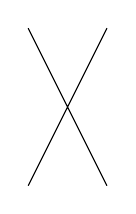
\begin{tikzpicture}
% These nodes will be reused in the next three tikzpicture environments.
\node[coordinate] (topleft) at (0,2) {};
\node[coordinate] (topright) at (1,2) {};
\node[coordinate] (botleft) at (0,0) {};
\node[coordinate] (botright) at (1,0) {};
\node (middle) at (0.5,1) {};

\draw (topleft) -- (botright)  (botleft) -- (topright);
\end{tikzpicture},
\end{center}
and transverse triple points. This involves working with a generalization of the braid group that includes generators for these vertices as well as the usual generators for crossings. In this case of 4-valent vertices, rigorously working out the generators and relations was done by Joan Birman in the paper below, but various people had used the answer already. The case of triple points is very important in physics due to the connection with the loop representation of quantum gravity (which is what Gambini is working on these days). In this representation, states are invariants of (possibly generalized) links, and only by considering links with triple points can one define operators such as the ``total volume of the universe''.

It is thus quite interesting that the authors make progress on determining the ``right'' extension of the HOMFLY polynomial invariant of links to links with transverse triple points -- that is, the extension that one gets by doing calculations in SU(n) Chern--Simons theory. In a special case, namely when the HOMFLY polynomial reduces to the Kauffman bracket (which corresponds to the Lie group SU(2)), one gets a state of quantum gravity that has been under extensive investigation these days. The authors compute the Kaufmann bracket of links with triple points using first order perturbation theory in Chern--Simons theory. A nonperturbative calculation would be very good to have!

\find{\paper{New points of view in knot theory, by Joan Birman, \href{https://arxiv.org/abs/math/9304209}{preprint}, to appear in the Bulletin of the AMS.}}

This is a nice review of the recent work on Vassiliev invariants of links. Given an invariant of oriented links, one can extend it to links with arbitrarily many double points by setting the value of the invariant on a link with a double point
\begin{center}
\begin{tikzpicture}
\draw (topleft) -- (botright)  (botleft) -- (topright);
\end{tikzpicture}
\end{center}
to be the invariant of the link with the double point changed to
\begin{center}
\begin{tikzpicture}
\draw (topleft) -- (middle) -- (botright)  (botleft) -- (topright);
\end{tikzpicture}
\end{center}
minus the invariant of the link with the double point changed to
\begin{center}
\begin{tikzpicture}
\draw (topleft) -- (botright)  (botleft) -- (middle) -- (topright);
\end{tikzpicture}.
\end{center}
Note that the link has to be oriented for this rule to make sense, and the strands shown in the pictures above should be pointing downwards. Now, having made this extension, we say a link invariant is a Vassiliev invariant of degree n if it vanishes on all links with n+1 or more double points.

It is interesting that this rule for extending link invariants to links with double points, when applied to the Kauffman bracket, does not give the extension computed by Gambini et al.\ in the paper above. (This is not surprising, actually, but it shows that some interesting things are going on in the subject of invariants for links with self-intersections and Chern--Simons theory.)

\find{\paper{Link polynomials and a graphical calculus, by Louis Kauffman and P. Vogel, \href{https://www.worldscientific.com/doi/abs/10.1142/S021821651240007X}{Jour. of Knot Theory and its Ramifications, 1 (1992), 59--104}.}}

This is another nice treatment of link invariants for generalized links with self-intersections. It concentrates on the famous link invariants coming from Chern--Simons theory -- the HOMFLY polynomial (from SU(n)) and the Kauffman polynomial (from SO(n)). Lots of good pictures.

And, switching back to the category theory, 2-categories, and the like, let me list these before filing them away:

\find{\paper{Categorical physics, by Louis Crane, preprint available as \href{https://arxiv.org/abs/hep-th/9301061}{arXiv:hep-th/9301061} in amstex.}
\paper{A Categorical construction of 4d topological quantum field theories, by Louis Crane and David Yetter, preprint available as \href{https://arxiv.org/abs/hep-th/9301062}{arXiv:hep-th/9301062} in latex.}
\paper{Hopf Categories and their representations, Louis Crane and Igor Frenkel, draft version.}
\paper{Categorification and the construction of topological quantum field theory, Louis Crane and Igor Frenkel, draft version.}}

These outline Louis Crane's vision of an approach to generally covariant 4-dimensional quantum field theories (e.g. quantum gravity or a ``theory of everything'') based on 2-categories. ``Categorical physics'' sketches the big picture, while the paper with Yetter provides a juicy mathematical spinoff -- the first known four-dimensional TQFT, based on the representations of quantum SU(2) and very similar in spirit to the Turaev--Viro construction of a 3d TQFT from quantum SU(2). The papers with Frenkel (apparently still not in their final form) describe the game plan and hint at marvelous things still to come. The conjecture is stated: ``a 4d TQFT can be reconstructed from a tensor 2-category''. This follows up on Crane's earlier work on getting 3d TQFTs from modular tensor categories (big example: the categories of representations of quantum groups at roots of unity). And the authors define the notion of a Hopf category, show how the category of module categories of a Hopf category is a tensor 2-category, and use ``categorification'' to turn the universal enveloping algebra of a quantum group into a Hopf category. Sound abstract? Indeed it is. But the aim is clear: to cook up 4d TQFTs from quantum groups. Such quantum field theories might be physically important; indeed, the one associated to SU(2) is likely to have a lot to do with quantum gravity.

I am currently perusing Kapranov and Voevodsky's massive paper on 2-categories, which seems to be the starting point for Crane's above papers and also those of Carter/Saito that I mentioned last week. Next week I should post an outline of what this paper does.

\find{\paper{The origin of time asymmetry, by S W Hawking, R Laflamme and G W Lyons, preprint available as \href{https://arxiv.org/abs/gr-qc/9301017}{arXiv:gr-qc/9301017}, in tex.}}

I haven't had a chance to read this one yet but it looks very ambitious and is likely to be interesting. Let me just quote from the introduction to get across the goal:

\begin{quote}
The laws of physics do not distinguish the future from the past direction of time. More precisely, the famous CPT theorem says that the laws are invariant under the combination of charge conjugation, space inversion and time reversal. In fact effects that are not invariant under the combination CP are very weak, so to a good approximation, the laws are invariant under the time reversal operation T alone. Despite this, there is a very obvious difference between the future and past directions of time in the universe we live in. One only has to see a film run backward to be aware of this.

There are are several expressions of this difference. One is the so-called psychological arrow, our subjective sense of time, the fact that we remember events in one direction of time but not the other. Another is the electromagnetic arrow, the fact that the universe is described by retarded solutions of Maxwell's equations and not advanced ones. Both of these arrows can be shown to be consequences of the thermodynamic arrow, which says that entropy is increasing in one direction of time. It is a non trivial feature of our universe that it should have a well defined thermodynamic arrow which seems to point in the same direction everywhere we can observe. Whether the direction of the thermodynamic arrow is also constant in time is something we shall discuss shortly.

There have been a number of attempts to explain why the universe should have a thermodynamic arrow of time at all. Why shouldn't the universe be in a state of maximum entropy at all times? And why should the direction of the thermodynamic arrow agree with that of the cosmological arrow, the direction in which the universe is expanding? Would the thermodynamic arrow reverse, if the universe reached a maximum radius and began to contract?

Some authors have tried to account for the arrow of time on the basis of dynamic laws. The discovery that CP invariance is violated in the decay of the K meson, inspired a number of such attempts but it is now generally recognized that CP violation can explain why the universe contains baryons rather than anti baryons, but it can not explain the arrow of time. Other authors have questioned whether quantum gravity might not violate CPT, but no mechanism has been suggested. One would not be satisfied with an ad hoc CPT violation that was put in by hand.

The lack of a dynamical explanation for the arrow of time suggests that it arises from boundary conditions. The view has been expressed that the boundary conditions for the universe are not a question for Science, but for Metaphysics or Religion. However that objection does not apply if there is a sense in which the universe has no boundary. We shall therefore investigate the origin of the arrow of time in the context of the no boundary proposal of Hartle \& Hawking. This was formulated in terms of Einsteinian gravity which may be only a low energy effective theory arising from some more fundamental theory such as superstrings. Presumably it should be possible to express a no boundary condition in purely string theory terms but we do not yet know how to do this. However the recent COBE observations indicate that the perturbations that lead to the arrow of time arise at a time during inflation when the energy density is about $10^{-12}$ of the Planck density. In this regime, Einstein gravity should be a good approximation.
\end{quote}

[I'll skip some more technical stuff on the validity of perturbative calculations in quantum gravity...]

\begin{quote}
One can estimate the wave functions for the perturbation modes by considering complex metrics and scalar fields that are solutions of the Einstein equations whose only boundary is the surface $S$. When $S$ is a small three sphere, the complex metric can be close to that of part of a Euclidean four sphere. In this case the wave functions for the tensor and scalar modes correspond to them being in their ground state. As the three sphere $S$ becomes larger, these complex metrics change continuously to become almost Lorentzian. They represent universes with an initial period of inflation driven by the potential energy of the scalar field. During the inflationary phase the perturbation modes remain in their ground states until their wave lengths become longer than the horizon size. The wave function of the perturbations then remains frozen until the horizon size increases to be more than the wave length again during the matter dominated era of expansion that follows the inflation. After the wave lengths of the perturbations come back within the horizon, they can be treated classically.

This behaviour of the perturbations can explain the existence and direction of the thermodynamic arrow of time. The density perturbations when they come within the horizon are not in a general state but in a very special state with a small amplitude that is determined by the parameters of the inflationary model, in this case, the mass of the scalar field. The recent observations by COBE indicate this amplitude is about $10^{-5}$. After the density perturbations come within the horizon, they will grow until they cause some regions to collapse as proto-galaxies and clusters. The dynamics will become highly non linear and chaotic and the coarse grained entropy will increase. There will be a well defined thermodynamic arrow of time that points in the same direction everywhere in the universe and agrees with the direction of time in which the universe is expanding, at least during this phase.

The question then arises: If and when the universe reaches and maximum size, will the thermodynamic arrow reverse? Will entropy decrease and the universe become smoother and more homogeneous during the contracting phase?
\end{quote}

[I'll skip some stuff on why Hawking originally thought entropy had to decrease during the Big Crunch if the no-boundary proposal were correct... and why he no longer thinks so.]

\begin{quote}
The thermodynamic arrow will agree with the cosmological arrow for half the history of the universe, but not for the other half. So why is it that we observe them to agree? Why is it that entropy increases in the direction that the universe is expanding? This is really a situation in which one can legitimately invoke the weak anthropic principle because it is a question of where in the history of the universe conditions are suitable for intelligent life. The inflation in the early universe implies that the universe will expand for a very long time before it contracts again. In fact, it is so long that the stars will have all burnt out and the baryons will have all decayed. All that will be left in the contracting phase will be a mixture of electrons, positrons, neutrinos and gravitons. This is not a suitable basis for intelligent life.
The conclusion of this paper is that the no boundary proposal can explain the existence of a well defined thermodynamic arrow of time. This arrow always points in the same direction. The reason we observe it to point in the same direction as the cosmological arrow is that conditions are suitable for intelligent life only at the low entropy end of the universe's history.
\end{quote}

\week{January 30, 1993}

Here's this week's reading material.  The first test will be in two
weeks.  :-)

\find{\paper{On the Vassiliev Knot Invariants by Dror Bar-Natan, Harvard
University ``pre-preprint.''}}

I went to UC San Diego this week to give a talk, and the timing was
nice, because Dror Bar-Natan was there.  He is a student of Witten who
has started from Witten's ideas relating knot theory and quantum field
theory and developed them into a beautiful picture that shows how knot
theory, the theory of classical Lie algebras, and abstract Feynman
diagrams are three faces of the same thing.  To put it boldly, in a
deliberately exaggerated form, Bar-Natan has proposed a conjecture
saying that knot theory and the theory of classical Lie algebras are
one and the same!  

This won't seem very exciting if you don't know what a classical Lie
algebra is.  Let me give a brief and very sketchy introduction,
apologizing in advance to all the experts for the terrible sins I will
commit, such as failing to distinguish between complex and real Lie
algebras. 

Well, remember that a Lie algebra is just a vector space
equipped with a ``bracket'' such that the bracket $[x,y]$ of any two vectors
$x$ and $y$ is again a vector, and such that the following hold:

\[\begin{array}{ll}
\text{a) skew-symmetry: }   & [x,y] = -[y,x].\\
\text{b) bilinearity: }     & [x,ay] = a[x,y], \ [x,y+z] = [x,y] + [x,z]\text{.  ($a$ is a number.)}\\
\text{c) Jacobi identity: } & [x,[y,z]] + [y,[z,x]] + [z,[x,y]] = 0.
\end{array}\]

The best known example is good old $\R^3$ with the cross product as the
bracket.  But the real importance of Lie algebras is that one can get
one from any Lie group -- roughly speaking, a group that's also a
manifold, and such that the group operations are smooth maps.  And the
importance of Lie groups is that they are what crop up as the groups of
symmetries in physics.  The Lie algebra is essentially the
''infinitesimal version'' of the corresponding Lie group, as anyone has
seen who has taken physics and seen the relation between the group of
rotations in $\R^3$ and the cross product.  Here the group is called SO(3)
and the Lie algebra is called so(3).  (So $\R^3$ with its cross product is
called so(3).)  One can generalize this to any number of dimensions,
letting SO($n$) denote the group of rotations in $\R^n$ and so($n$) the
corresponding Lie algebra.  (However, so($n$) is not isomorphic to $\R^n$
except for $n = 3$, so there is something very special about three
dimensions.)  

Similarly, if one uses complex numbers instead of real numbers, 
one gets a group SU($n$) and Lie algebra su($n$).  And if one looks at the 
symmetries of a $2n$-dimensional classical phase
space -- so-called canonical transformations, or symplectic
transformations -- one gets the group Sp($n$) and Lie algebra sp($n$).  
To be precise, SO($n$) consists of all nxn orthogonal real matrices with
determinant 1, SU($n$) consists of all nxn unitary complex matrices with
determinant 1, and Sp($n$) consists of all $(2n) \times (2n)$ real matrices
preserving a nondegenerate skew-symmetric form.

These are all very important in physics.  Indeed, all the ``gauge groups''
of physics are Lie groups of a certain sort, so-called compact
Lie groups, and in the standard model all the forces are
symmetrical under some gauge group or other.  Electromagnetism \`a la
Maxwell is symmetric under the group U(1) of complex numbers of unit
magnitude, or ``phases''.  The electroweak force (unified electromagnetism
and weak force) is symmetric under U(1) $\times$ SU(2), where one uses the fact
that one can build up bigger semisimple Lie groups as direct sums
(also called products) of smaller ones.  The gauge group for the
strong force is SU(3).  And, finally, the gauge group of the whole
standard model is simply U(1) $\times$ SU(2) $\times$ SU(3), which results from
lumping the electroweak and strong gauge groups together.  This direct
sum business also works for the Lie algebras, so the Lie algebra
relevant to the standard model is written u(1) $\times$ su(2) $\times$ su(3).

There are certain very special Lie algebras called simple Lie algebras
which play the role of ``elementary building blocks'' in the world of Lie
algebras.  They cannot be written as the direct sum of other Lie
algebras (and in fact there is an even stronger sense in which they
cannot be decomposed).  On the other hand, the Lie algebra of any
compact Lie group is a direct sum of simple Lie algebras and copies of
u(1) -- the one-dimensional Lie algebra with zero Lie bracket which, for
technical reasons, people don't call ``simple''.  

These simple Lie algebras were classified by the monumental work of
Killing, Cartan and others, and the classification is strikingly simple:
there are infinite series of ``classical'' Lie algebras of type
su($n$), so($n$), and sp($n$), and five ``exceptional'' Lie algebras
called $G_2$, $F_4$, $E_6$, $E_7$, and $E_8$.  Believe it or not, there is a deep
connection between the exceptional Lie algebras and the Platonic solids.
But that is another story, one I barely know....

Now, Witten showed how one could use quantum field theory to constuct an
invariant of knots, or even links, corresponding to any representation
of a compact Lie group.  (You won't even need to know what a
representation is to understand what follows.)  This had been done in a
different way, in terms of ``quantum groups,'' by Reshetikhin and Turaev
(following up on work by many other people).  These invariants are
polynomials in a variable $q$ (for ``quantum''), and if one writes $q$ as
$e^\hbar$ and expands a power series in $\hbar$, the coefficient of $\hbar^n$ is
a ``Vassiliev invariant of degree $n$''.  Recall from last week that
given an invariant of oriented knots, one can extend
it to knot with arbitrarily many nice crossings by setting
the value of the invariant on a knot with a crossing like

\begin{center}
\begin{tikzpicture}
\draw (topleft) -- (botright)  (botleft) -- (topright);
\end{tikzpicture}
\end{center}
to be the invariant of the knot with the crossing changed to
\begin{center}
\begin{tikzpicture}
\draw (topleft) -- (middle) -- (botright)  (botleft) -- (topright);
\end{tikzpicture}
\end{center}
minus the invariant of the knot with the crossing changed to
\begin{center}
\begin{tikzpicture}
\draw (topleft) -- (botright)  (botleft) -- (middle) -- (topright);
\end{tikzpicture}.
\end{center}
(Again, the knot has to be oriented for this rule to make sense,
and the strands shown in the pictures above should be pointing
downwards.)   Having made this extension, one says a knot
invariant is a Vassiliev invariant of degree $n$ if it vanishes
on all knots with $n+1$ or more double points.

This is where Dror stepped in, roughly.  First of all, he showed that
the Vassiliev invariant of degree $n$ is just what you get when you do
Witten's quantum-field-theoretic calculations perturbatively using
Feynman diagrams and look at the terms of order $n$ in Planck's constant,
$\hbar$!  Secondly, and more surprisingly, he developed a bunch of
relationships between Feynman diagrams and pictures of knots!  The third
and most amazing thing he did takes a bit longer to explain...
\vskip 3ex
Roughly, he showed that any Vassiliev invariant of degree $n$ is
determined by some combinatorial data called a ``weight system.''  He
showed that any representation of a Lie algebra determines a weight
system and hence a Vassiliev invariant.  But the really interesting
thing he showed is that many of the things one can do for Lie algebras
can be done for arbitrary weight systems.  This makes it plausible that
EVERY weight system, hence every Vassiliev invariant, comes from a
representation of a simple Lie algebra.  In fact, Dror conjectures that
every Vassiliev invariant comes from a representation of a classical
simple Lie algebra.  Now there is another conjecture floating around
these days, namely that Vassiliev invariants almost form a complete set
-- that is, that if two knots cannot be distinguished by any Vassiliev
invariants, they must either be the same or differ simply by reversing the
orientation of all the strands.  If BOTH these conjectures are true,
one has in some sense practically reduced the theory of knots to the
theory of the classical Lie algebras!  This wouldn't mean that all of
sudden we know the answer to every question about knots, but it would
certainly help a lot, and more importantly, in my opinion, it would show
that the connection between topology and the theory of Lie algebras is far
more profound than we really understand.  The ramifications for physics,
as I hope all my chatting about knots, gauge theories and quantum
gravity makes clear, might also be profound.

Well, we \emph{certainly} don't understand all this stuff yet, since we don't know
how to prove these conjectures!  But Dror's conjecture -- that all weight
systems come from representations of simple Lie algebras -- is
tantalizingly close to being within grasp, since he has reduced it to a
fairly elementary combinatorial problem, which I will now state.  Note
that ``elementary'' does not mean easy to solve!  Just easy to state.

Before I state the combinatorial problem, let me say
something about the evidence for the conjecture that all Vassiliev
invariants come from representations of classical Lie algebras.  In
addition to all sorts of ``technical'' evidence, Dror has shown the 
conjecture is true for Vassiliev invariants of degree $\leq 9$ by means
of many hours of computation using his Sparcstation.  In fact, he said
in his talk that he felt guilty about having a Sparcstation unless it
was always computing something, and that even as he spoke his computer
was busily verifying the conjecture for higher degrees.  (I suggested
that it was the Sparcstation that should feel guilty when it was not
working, not him.)  He also advertised that his programs, a mixture of C
and Mathematica code, are available by anonymous ftp from math.harvard.
Use user name ``ftp'', go to the directory ``dror''.  You folks with Crays 
should feel VERY guilty if they are just sitting there and not helping
Dror verify this important conjecture. (I suggest that you first read his
papers and the file README in his directory, then check out his
programs, and then ask him where he's at and what would be worth doing.
Please don't pester him unless you are a good enough mathematician to
discuss this stuff intelligently and have megaflops to burn.  If you
want to make a fool of yourself, \emph{don't} say I sent you.)  
\vskip 3ex
Okay, with no further ado, here's the conjecture in its elementary
combinatorial form.  Let $B$ be the vector space spanned by finite graphs with
univalent and ``oriented'' trivalent vertices, modulo some
relations... first of all, a trivalent vertex is ``oriented'' if there is
a cyclic ordering of the three incident edges.  That is, we ``orient'' the
vertex 
\begin{center}
\begin{tikzpicture}
\node[coordinate] (top) at (0.5,2) {};
\node[coordinate] (mid) at (0.5,1) {};
\node[coordinate] (bottom) at (0.5,0) {};
\node[coordinate] (left) at (0,1) {};
\node[coordinate] (right) at (1,1) {};

\draw (topleft) -- (mid) -- (topright)  (mid) -- (bottom);
\end{tikzpicture}
\end{center}
by drawing a little clockwise or counterclockwise-pointing circle at the
vertex.  (Or, for those of an algebraic bent, label the edges by 1,2,3
but then mod out by cyclic permutations.)  The relations are: 1)  if we
reverse the orientation of a trivalent vertex, that's equivalent to
multiplying the graph by $-1$.  (Remember we're in a vector space spanned
by graphs.)  2)  
\begin{center}
\begin{tikzpicture}
\draw (topleft) -- (topright)  (botleft) -- (botright)  (top) -- (bottom);
\end{tikzpicture}
\quad \raisebox{1cm}{=} \quad
\begin{tikzpicture}
\draw (topleft) -- (botleft)  (topright) -- (botright)  (left) -- (right);
\end{tikzpicture}
\quad \raisebox{1cm}{$-$} \quad
\begin{tikzpicture}
\draw (topleft) -- (botright)  (botleft) -- (topright);
\end{tikzpicture}
\end{center}
(That is, we can make this substitution anywhere we want; these pictures
might be part of a bigger graph.  Note that the ``X'' is not a vertex,
since there aren't quadrivalent vertices; it's just one edge going over
or under another.  It doesn't matter whether it goes over or under since
these are abstract graphs, not graphs embedded in space.)  

Now, let $B_m$ be the vector space spanned by ``labelled'' finite graphs
with univalent and oriented trivalent vertices, modulo some relations...
but first I have to say what ``labelled'' means.  It means that each edge
is labelled with a $1$ or $-1$.  The relations are: 1) if we reverse the
orientation of a trivalent vertex, it's the same as multiplying the
labellings of all three incident edges by $-1$.  2)   
\begin{center}
\begin{tikzpicture}
\draw (topleft) -- (topright)  (botleft) -- (botright)  (top) -- (bottom);
\end{tikzpicture}
\quad \raisebox{1cm}{=} \quad
\begin{tikzpicture}
\draw (topleft) -- (botleft)  (topright) -- (botright)  (left) -- (right);
\end{tikzpicture}
\end{center}
\emph{if} the internal edge is labelled with a 1.  (Here the 4 external edges
can have any labellings and we don't mess with that.)

Now, define a linear map from $B$ to $B_m$ by mapping any graph to the
signed sum of the $2^{\text{number of edges}}$ ways of labelling the edges with 1
or $-1$.  Symbolically,
\begin{center}
\begin{tikzpicture}
\draw (0,0) -- (6em,0)  (9em,0) -- (15em,0)  (18em,0) -- (24em,0);
\node at (7.5em,0) {$\to$};
\node at (16.5em,0) {$-$};
\node at (12em,1.8ex) {$1$};
\node at (21em,1.8ex) {$-1$};
\end{tikzpicture}.
\end{center}
Of course, one must work a bit to show this map is well-defined.  (This
just takes a paragraph -- see Proposition 6.5 of Dror's paper.)  

Okay, the conjecture is:
\begin{center}
			THIS MAP IS ONE-TO-ONE.
\end{center}
If you can solve it, you've made great progress in showing that knots
and classical Lie groups are just two aspects of the same branch of
mathematics.  Don't work on it, though, until you get Dror's paper and
make sure I stated it exactly right!!!!!

\find{\paper{Mathematical problems of non-perturbative quantum general
relativity, by Abhay Ashtekar, lectures delivered at the 1992 Les
Houches summer school on Gravitation and Quantization, December 2, 1992,
available as \href{https://arxiv.org/abs/gr-qc/9302024}{arXiv:gr-qc/9302024}.}}

This is a good overview of the loop variables approach to quantizing
general relativity as it currently stands.   It begins with a review of
the basic difficulties with quantizing gravity, as viewed from three
perspectives: the particle physicist, the mathematical physicist, and
the general relativist.  Technically, a main problem is that general
relativity consists of both evolution equations and constraint equations
on the initial data (which are roughly the metric of space at a given
time and its first time derivative, or really ``extrinsic curvature'').  
So Ashtekar reviews Dirac's ideas on quantizing constrained systems
before sketching how this program is carried out for general relativity.

Then he considers a ``toy model'' -- quantum gravity in 2+1 dimensions.
This is a funny theory because \emph{classically} Einstein's equations in 2+1
dimensions simply say that spacetime is flat (in a vacuum)!  No
gravitational waves exist as in 3+1 dimensions, and one can say that the
information in the gravitational field is ``purely global'' -- locally,
everywhere looks the same as everywhere else (like Iowa), but there may
be global ``twists'' that you notice when going around a noncontractible loop.
There has been a lot of work on 2+1 gravity recently -- in a sense this problem
has been solved, by a number of methods -- and this allows one to
understand \emph{some} of the conceptual difficulties of honest
3+1-dimensional quantum gravity without getting caught in an endless net
of technical complications.  

Then Ashtekar jumps back to 3+1 dimensions and gives a more thorough
introduction to the loop variables approach.  He ends by going through
some of the many open problems and possible ways to attack them.  
\vskip 3ex
I have worn myself out trying to do justice to Bar-Natan's work, so I
will postpone until next week a review of Kapranov and Voevodsky's paper
on 2-categories.  

\week{February 8, 1993}

I will begin with a couple of small things and then talk about
the work of Kapranov and Voevodsky.

\find{\paper{Self-organized criticality in Monte Carlo simulated ecosystems, by
R. Sole, D. Lopez, M. Ginovart and J. Valls, Phys. Lett. A172 (1992), p. 56.}}

This is mainly of interest to me thanks to a reference to some earlier work
on Conway's game of Life.  At MIT, Tom Toffoli, Norm Margolus, and grad
students in the Physics of Computation group build special-purpose
computers for simulating cellular automata, the so-called CAM machines.
I have spent many enjoyable hours watching beautiful patterns do their
thing on a big-screen color TV while CAM 6 busily simulates them on a
256 $\times$ 256 lattice at the rate of many generations a second.  (The CAM 8
chip was still being debugged when I last checked.)     More recently,
Jim Gilliam, a grad student here at UCR, found a very nice program for the
game of Life on Xwindows, called xlife.  On my Sparcstation it is even
bigger and faster than CAM6.  One can zoom in and out, and, zooming all
the way out, one sees something vaguely reminiscent of nebulae of
distant stars twinkling in the night sky...  My computer science pal,
Nate Osgood, muttered something about the author, Chuck Silvers
(\href{mailto:cs4n@andrew.cmu.edu}{cs4n@andrew.cmu.edu}), using cleverly optimized loops.  It apparently
can be found using the program archie.  Please don't ask \emph{me} for a copy,
since it involves many files.  

The game of Life is actually one of the less fun cellular automata
to watch, since, contrary to its name, if one starts with a random
configuration it almost always eventually lapses into an essentially
static configuration (perhaps with some blinkers executing simple
periodic motions).   I am pleased to find that this seemingly dull final
state might be fairly interesting in the study  of self-organized
criticality!  Recall that this is the phenomenon whereby a physical
system naturally works its way into a state such that the slightest
disturbance can have an arbitrarily large effect.  The classic example
is a sand dune, which apparently works its way towards slopes close to
the critical one at which an avalanche occurs.  Drop one extra grain of
sand on it and you can get a surprisingly wide distribution of possible
sizes for the resulting sandslide!  Similar but more formidable effects
may be at work in earthquakes.   The above paper cites
\vskip 2ex
Bac, Chen and Creutz, Nature 342 (1989) p. 780,
\vskip 2ex
\noindent which claims that in the final state of the game of Life, the
density of clusters $D(s)$ of size $s$ scales as about $s^{-1.4}$, and that the
probability that a small perturbation will cause a flurry of activity
lasting a time $t$ scales as about $t^{-1.6}$.   I'm no expert, but I guess
that the fact that the latter is a power law rather than an exponential
would be a signal of self-organized criticality.  But the paper also
cites
\vskip 2ex
Bennett and Bourzutschy, Nature 350 (1991) 468,
\vskip 2ex
who claim that the work of Bac, Chen and Creutz is wrong.  I haven't
gotten to read these papers; if anyone wants to report on them I'd be
interested.  

The paper I read considers fancier variations on this theme,
investigating the possibility that ecosystems are also examples of
self-organized criticality.  It's hard to know how to make solid science
out of this kind of thing, but I think there would be important
consequences if it turned out that the ``balance of nature,'' far from
being a stable equilibrium, was typically teetering on the brink of
drastic change.  

\find{\paper{There are no quantum jumps, nor are there particles!, by H. D. Zeh,
Phys. Lett. A173, p. 189.}}

Having greatly enjoyed Zeh's book The Physical Basis for the Direction
of Time -- perhaps the clearest account of a famously murky subject -- I
naturally took a look at this particle despite its overheated title.  
(Certainly exclamation marks in titles should add to one's crackpot index.)
It is a nice little discussion of ``quantum jumps'' and the ``collapse of
the wavefunction'' that takes roughly the viewpoint I espouse, namely,
that all one needs is Schrodinger's equation (and lots of hard work) to
understand what's going on in quantum theory -- no extra dynamical
mechanisms.  It's not likely to convince anyone who thinks otherwise,
but it has references that might be useful no matter which side of the 
debate one is on.

Also, this just in -- what you've all been waiting for -- another
interpretation of quantum mechanics!  It's a book by David Bohm and
Basil Hiley, entitled ``The Undivided Universe - An Ontological
Interpretation of Quantum Theory.''  I have only seen an advertisement so
far; it's published by Routledge.  The contents include such curious
things as ``the ontological interpretation of boson fields.''  Read it at
your own risk.

\find{\paper{Braided monoidal 2-categories, 2-vector spaces and Zamolodchikov
tetrahedra equations, by M.\ M.\ Kapranov and V.\ A.\ Voevodsky.
Preliminary incomplete version, September 1991.  (Kapranov is at
\href{mailto:kapranov@chow.math.nwu.edu}{kapranov@chow.math.nwu.edu}, and Voevodsky is at \href{mailto:vladimir@math.ias.edu}{vladimir@math.ias.edu}.)}}

This serious and rather dry paper is the basis for what a lot of 
physicists are just beginning to try to do: burst from the confines of 3
dimensions, where knots and topological quantum field theories like
Chern--Simons theory live, to 3+1 dimensions, where we live.  The
``incomplete version'' I have is 220 pages long, mostly commutative
diagrams, and doesn't have much to say about physics.  But I have a hunch
that it will become required reading for many people fairly soon, so 
I'd like to describe the main ideas in fairly simple terms.  

I will start from scratch and then gradually accelerate.  First, what's
a category?  A category consists of a set of `objects' and a set of
`morphisms'.  Every morphism has a `source' object and a `target'
object.  (The easiest example is the category in which the objects
are sets and the morphisms are functions.  If $f \maps X \to Y$, we call $X$ the
source and $Y$ the target.)  Given objects $X$ and $Y$, we write $\Hom(X,Y)$
for the set of morphisms `from' $X$ `to' $Y$ (i.e., having $X$ as source and $Y$
as target).  

The axioms for a category are that it consist of a set of objects and
for any 2 objects $X$ and $Y$ a set $\Hom(X,Y)$ of morphisms from $X$ to $Y$, and
\begin{enumerate}[a)]
\item Given a morphism $g$ in $\Hom(X,Y)$ and a morphism $f$ in $\Hom(Y,Z)$, there
is morphism which we call $f \of g$ in $\Hom(X,Z)$.  (This binary operation $\of$ is
called `composition'.)
\item Composition is associative:  $(f \of g) \of h = f \of (g \of h)$.
\item For each object $X$ there is a morphism $\id_X$ from $X$ to $X$, called the
`identity' on $X$.
\item Given any $f$ in $\Hom(X,Y)$, $f \of \id_X = f \text{ and } \id_Y \of f = f$.
\end{enumerate}
Again, the classic example is $\Set$, the category with sets as objects and
functions as morphisms, and the usual composition as composition!
But lots of the time in mathematics one is some category or other, e.g.:
\vskip 1em \noindent
$\Vect$ --- vector spaces as objects, linear maps as morphism\\
$\Group$ --- groups as objects, homomorphisms as morphisms\\
$\Top$ ---  topological spaces as objects, continuous functions as morphisms\\
$\Diff$ --- smooth manifolds as objects, smooth maps as morphisms\\
$\Ring$ --- rings as objects, ring homomorphisms as morphisms
\vskip 1em \noindent
or in physics:
\vskip 1em \noindent
$\Symp$ --- symplectic manifolds as objects, symplectomorphisms as morphisms\\
$\Poiss$ --- Poisson manifolds as objects, Poisson maps as morphisms\\
$\Hilb$ --- Hilbert spaces as objects, unitary operators as morphisms
\vskip 1em \noindent
(The first two are categories in which one can do classical physics.
The third is a category in which one can do quantum physics.)

Now, what's a 2-category?  This has all the structure of a category but
now there are also ``2-morphisms,'' that is, morphisms between morphisms!
This is rather dizzying at first.  Indeed, much of category theory is
rather dizzying until one has some good examples to lean on (at least
for down-to-earth people such as myself), so let us get some examples
right away, and leave the definition to Kapranov and Voevodsky!   My
favorite example comes from homotopy theory.  Take a topological space $X$
and let the objects of our category be points of $X$.  Given $x$ and $y$ in $X$,
let $\Hom(x,y)$ be the set of all unparametrized paths from $x$ to $y$.  We
compose such paths simply by sticking a path from $x$ to $y$ and a path from
$y$ to $z$ to get a path from $x$ to $z$, and we need unparametrized paths to
make composition associative. Now given two paths from $x$ to $y$, say $f$ and
$g$, let $\HOM(f,g)$, the set of  2-morphisms from $f$ to $g$, be the set of
unparametrized homotopies from $f$ to $g$ -- that is, ways of deforming the
path $f$ continuously to get the path $g$, while leaving the endpoints fixed.  

This is a very enlightening example since homotopies of paths are really
just ``paths of paths,'' making the name 2-morphism quite appropriate.
(Some of you will already be pondering 3-morphisms, 4-morphisms, but it's
too late, they've already been invented!  I won't discuss them here.)
The notation for 2-morphisms is quite cute: given $f,g$ in $\Hom(x,y)$, we
write $F$ in $\HOM(f,g)$ as the following diagram:
\[
\begin{tikzcd}
   x
   \arrow[rr, bend left,"f"]
   \arrow[rr, bend right,"g",swap]
   &
   \zwei F
   &
   y
\end{tikzcd}
\]
This is two arrows from $x$ to $y$, namely $f$ and $g$, and then
a big fat double arrow labelled $F$ going down from $f$ to $g$.  In other
words, while ordinary morphisms are 1-dimensional objects (arrows),
2-morphisms are 2-dimensional ``cells'' filling in the space between two 
ordinary morphisms.  We thus see that going up to ``morphisms between
morphisms'' is closely related to going up to higher dimensions.  And
this is really why ``braided monoidal 2-categories'' may play as big a
role in four-dimensional field theory as ``braided monoidal categories''
do in three-dimensional field theory!

Rather than write down the axioms for a 2-category, which are in
Kapranov and Voevodsky, let me note the key new thing about 2-morphisms:
there are two ways to compose them, ``horizontally'' and ``vertically''.
First of all, given the following situation:
\[
\begin{tikzcd}
   x
   \arrow[rr, bend left,"f"]
   \arrow[rr, bend right,"g",swap]
   &
   \zwei F
   &
   y
   \arrow[rr, bend left,"f'"]
   \arrow[rr, bend right,"g'",swap]
   &
   \zwei F'
   &
   z
\end{tikzcd}
\]
we can compose $F$ and $F'$ horizontally to get a 2-morphism from $f' \of f$ to
$g' \of g$.  (Check this out in the example of homotopies!)  But also, given
the following situation:
\[
\begin{tikzcd}[row sep = 0.1em]
   &
   \zwei F
   \\
   x
   \arrow[rr, bend left=70,"f"]
   \arrow[rr,"g"]
   \arrow[rr, bend right=70,"h",swap]
   &&
   y
   \\
   &
   \zwei G
\end{tikzcd}
\]
($f,g,h$ in $\Hom(x,y)$, $F$ in $\HOM(f,g)$, and $G$ in $\HOM(g,h)$), we can
compose $F$ and $G$ vertically to get a 2-morphism from $f$ to $g$.  

As Kapranov and Voevodsky note: ``Thus 2-categories can be seen as
belonging to the realm of a new mathematical discipline which may be
called 2-DIMENSIONAL ALGEBRA and contrasted with usual 1-dimensional
algebra dealing with formulas which are written in lines.''  This is
actually very important because already in the theory of braided
monoidal categories we began witnessing the rise of mathematics that
incorporated aspects of geometry into the notation itself. 

The theory of 2-categories is not new; it was apparently invented by
Ehresmann, Benabou and Grothendieck in an effort to formalize the
structure possessed by the category of all categories.  (If this notion
seems dangerously close to Russell's paradox, you are right -- but I will
not worry about such issues in what follows.)  This category has as its
objects categories and as its morphisms ``functors'' between categories.  It
is, in fact, a 2-category, taking as the 2-morphisms ``natural
transformations'' between functors.  (For a brief intro to functors and
natural transformations, try the file ``categories'' in the collection of
my expository papers -- see the end of this post.)  What is new to
Kapranov and Voevodsky is the notion of a monoidal 2-category --
where one can take tensor products of objects, morphisms, and
2-morphisms -- and ``braided'' monoidal 2-category -- where one has
``braidings'' that switch around the two factors in a tensor product.  

Let me turn to the possible relevance of all this to mathematical
physics.  Here there is a nice 2-category, namely the category of 
``2-tangles.''  First recall the category of tangles (stealing from something
that appears in the file ``tangles'' in the collection of my papers):

The objects are simply the natural numbers $\{0,1,2,3,\dotsc\}$.  We think
of the object $n$ as a horizontal row of $n$ points.  The morphisms
in $\Hom(n,m)$ are tangles connecting a row of $n$ points above to a row of
$m$ points below.  Rather than define ``tangles'' I will simply draw pictures of
some examples. Here is an element of $\Hom(2,4)$: 
\begin{verbatim}
        |   |
        \   /
         \ /
          \     /\
         / \   /  \
        |   \ /    \
        |    \      |
        |   / \     |
\end{verbatim}
and here is an element of $\Hom(4,0)$:
\begin{verbatim}
        |  |   |    |
        \  /   \ /\ /
         \/     \  \
               / \/ \
               \____/
\end{verbatim}
Note that we can ``compose'' these tangles to get one in $\Hom(2,0)$:
\begin{verbatim}
        |   |
        \   /
         \ /
          \     /\
         / \   /  \
        |   \ /    \
        |    \      |
        |   / \     |
        |  |   |    |
        \  /   \ /\ /
         \/     \  \
               / \/ \
               \____/
\end{verbatim}
Now, given tangles $f,g$ in $\Hom(m,n)$, a 2-morphism from $f$ to $g$ is 
a ``2-tangle.''   I won't define these either, but we may think of a 2-tangle
from $f$ to $g$ roughly as a ``movie'' whose first frame is the tangle $f$ and
last frame is the tangle $g$, and each of whose intermediate frames is a
tangle except at certain times when a catastrophe occurs.   For example,
here's a 2-tangle shown as a movie... 
\vskip 3ex \noindent
Frame 1
\\[1ex]
\begin{tikzpicture}
\draw (topleft) -- (botleft)  (botright) -- (topright);
\end{tikzpicture}
\\
Frame 2 
\\[1ex]
\begin{tikzpicture}[bend angle=30]
\path (topleft) edge[bend left, looseness=0.7] (botleft);
\path (botright) edge[bend left, looseness=0.7] (topright);
\end{tikzpicture}
\\
Frame 3
\\[1ex]
\begin{tikzpicture}
\draw (topleft) .. controls (mid) .. (botleft);
\draw (botright) .. controls (mid) .. (topright);
\end{tikzpicture}
\\
Frame 4 (the exciting scene -- the catastrophe!)
\\[1ex]
\begin{tikzpicture}
\draw (topleft) -- (botright)  (botleft) -- (topright);
\end{tikzpicture}
\\
Frame 5
\\[1ex]
\begin{tikzpicture}
\draw (topleft) .. controls (mid) .. (topright);
\draw (botright) .. controls (mid) .. (botleft);
\end{tikzpicture}
\\
Frame 6
\\[1ex]
\begin{tikzpicture}[bend angle=60]
\path (topleft) edge[bend right, looseness=1.2] (topright);
\path (botright) edge[bend right, looseness=1.2] (botleft);
\end{tikzpicture}

Well, it'll never win an Academy Award, but this movie is pretty
important.  It's a picture of the 3-dimensional slices of
a 2-dimensional surface in (3+1)-dimensional spacetime, and this
surface is perfectly smooth but has a saddle point which we are seeing
in frame 4.  It is one of what Carter and Saito (see {\hyperref[find1.1]{week~1}})
call the ``elementary string interactions.''  The relevance to string
theory is pretty obvious: we are seeing a movie of part of a string
worldsheet, which is a surface in (3+1)-dimensional spacetime.  My
interest in 2-tangles and 2-categories is precisely because they offer a
bridge between string theory and the loop variables approach to quantum
gravity, which may actually be the SAME THING in two different
disguises.  You heard it here first, folks!

The reader may have fun figuring out what the two ways of composing
2-morphisms amount to in the category of 2-tangles.  
\vskip 3ex
There are, in fact, many clues as to the relation between string theory
and 2-categories, one being the Zamolodchikov equation.  This is the 
analog of the Yang--Baxter equation -- an equation important in the theory
of braids -- one dimension up.  It was discovered by Zamolodchikov in
1980; a 1981 paper that might be a bit easier to get is ``Tetrahedron
equations and relativistic S-matrix for straight strings in 2+1
dimensions,'' Comm. Math. Phys. 79 (1981), 489-505.   (It plays a
different role in the (3+1)-dimensional context, though.)  Just as
braided monoidal categories are a good way to systematically find
solutions of the Yang--Baxter equation, braided monoidal 2-categories,
as defined by Kapranov and Voevodsky, seem to be a good way for finding
solutions for the Zamolodchikov equation.  (I will post in a while
about a new paper by Soibelman and Kazhdan that does this.  Also see the
paper by Crane and Frenkel in {\hyperref[find2.4]{week~2}}.)

There are also lots of tantalizing ties between the loop variables approach
to quantum gravity and 2-categories; one can see some of these if one
reads the work of Carter and Saito in conjunction with my paper ``Quantum
Gravity and the Algebra of Tangles''.  I hope to make these a lot clearer
as time goes by.

\week{February 13, 1993}

I think I'll start out this week's list of finds with an elementary introduction to Lie algebras, so that people who aren't "experts" can get the drift of what these are about. Then I'll gradually pick up speed... 
\vskip 2ex
\find{\paper{Vyjayanathi Chari and Alexander Premet, Indecomposable restricted representations of quantum sl2, University of California at Riverside preprint.}}
\vskip 2ex
Vyjayanathi is our resident expert on quantum groups, and Sasha, who's visiting, is an expert on Lie algebras in characteristic p. They have been talking endlessly across the hall from me and now I see that it has born fruit. This is a pretty technical paper and I am afraid I'll never really understand it, but I can see why it's important, so I'll try to explain that!

Let me start with the prehistory, which is the sort of thing everyone should learn. Recall what a Lie algebra is... a vector space with a "bracket" operation such that the bracket $[x,y]$ of any two vectors $x$ and $y$ is again a vector, and such that the following hold:

\[\begin{array}{ll}
\text{a) skew-symmetry: }   & [x,y] = -[y,x].\\
\text{b) bilinearity: }     & [x,ay] = a[x,y], \ [x,y+z] = [x,y] + [x,z]\text{.  ($a$ is a number.)}\\
\text{c) Jacobi identity: } & [x,[y,z]] + [y,[z,x]] + [z,[x,y]] = 0.
\end{array}\]

These conditions, especially the third, may look sort of weird if you are not used to them, but the examples make it all clear. The easiest example of a Lie algebra is $\mathfrak{gl}_n(\mathbb{C})$, which just means all $n\times n$ complex matrices with the bracket defined as the "commutator": 

\[[x,y] = xy - yx.\]  

Then straightforward calculations show a) -c) hold... so these conditions are really encoding the essence of the commutator.

Now recall that the trace of a matrix, the sum of its diagonal entries, satisfies $\tr(xy) = \tr(yx)$. So the trace of any commutator is zero, and if we let $\mathfrak{sl}_n(\mathbb{C})$ denote the matrices with zero trace, we see that it's a sub-Lie algebra of $\mathfrak{gl}_n(\mathbb{C})$ - that is, if $x$ and $y$ are in $\mathfrak{sl}_n$ so is $[x,y]$, so we can think of $\mathfrak{sl}_n(\mathbb{C})$ as a Lie algebra in its own right. Going from $\mathfrak{sl}_n(\mathbb{C})$ to $\mathfrak{gl}_n(\mathbb{C})$ is essentially a trick for booting out the identity matrix, which commutes with everything else (hence has vanishing commutators). The identity matrix is the only one with this property, so it's sort of weird, and it simplifies things to get rid of it here.

The simplest of the $\mathfrak{sl}_n(\mathbb{C})$'s is the Lie algebra $\mathfrak{sl}_2(\mathbb{C})$, affectionately known simply as $\mathfrak{sl}_2$, which is a 3-dimensional Lie algebra with a basis given by matrices people call $E$, $F$, and $H$ for mysterious reasons:
\\
$E = \begin{bmatrix}
    0 & 1 \\
    0 & 0 \\
  \end{bmatrix}$
$F =
  \begin{bmatrix}
    0 & 0 \\
    1 & 0 \\
  \end{bmatrix}$
$H = 
  \begin{bmatrix}
    1 & 0 \\
    0 & -1 \\
  \end{bmatrix}$
\\


You will never be an expert on Lie algebras until you know by heart that

$[H,E] = 2E$,    $[H,F] = -2F$,     $[E,F]  = H$.

Typically that's the sort of remark I make before screwing up by a factor of two or something, so you'd better check! This is a cute little multiplication table... but very important, since $\mathfrak{sl}_2$ is the primordial Lie algebra from which the whole theory of "simple" Lie algebras unfolds.

Physicists are probably more familiar with a different basis of $\mathfrak{sl}_2$, the Pauli matrices: 
$ \sigma_1 = \begin{pmatrix} 
0 & 1 \\
1 & 0 
\end{pmatrix} $
$ \sigma_2 = \begin{pmatrix} 
0 & -i \\
i & 0 
\end{pmatrix} $
$ \sigma_3 = \begin{pmatrix} 
1 & 0 \\
0 & -1 
\end{pmatrix} $

For purposes of Lie algebra theory it's actually better to divide each of these matrices by $i$ and call the resulting matrices $I$, $J$, and $K$, respectively. We then have

$IJ = -JI = K$,	$JK = -KJ = I$, $KI = -IK = J$, $I2 = J2 = K2 = -1$

Which is just the multiplication table of the quaternions! From the point of view of Lie algebras, though, all that matters is:

$[I,J] = 2K$,    $[J,K] = 2I$,    $[K,I] = 2J$.

Given the relation of these things and cross products, it should be no surprise that the Pauli matrices have a lot to with angular momentum around the $x$, $y$, and $z$ axes in quantum mechanics.

If we take all \textit{real} linear combinations of $E$,$F$,$H$ we get a Lie algebra over the \textit{real} numbers called $\mathfrak{sl}_2(\mathbb{R})$, and if we take all real linear combinations of $I$, $J$, $K$ we get a Lie algebra over the reals called $SU(2)$. These two Lie algebras are two different "real forms" of $\mathfrak{sl}_2$.

Now, people know just about everything about $\mathfrak{sl}_2$ that they might want to. Well, there's always something more, but I'm certainly personally satisfied! I recall when as an impressionable student I saw a book by Serge Lang titled simply "$SL_2(\mathbb{R})$," big and fat and scary inside. 
I knew what $SL_2(\mathbb{R})$, was, but not how one could think of a whole book's worth of things to write about it! A whole book on 2x2 matrices??

Part of how one gets so much to say about a puny little Lie algebra like $\mathfrak{sl}_2$ is by talking about its representations. What's a representation? Well, first you have to temporarily shelve the idea that $\mathfrak{sl}_2$ consists of 2x2 matrices, and think of it more abstractly simply as a 3-dimensional vector space with basis $E,F,H$, equipped with a Lie algebra structure given by the multiplication table $[H,E] = 2E, [H,F] = -2F, [E,F] = H$. If this is how I'd originally defined it, it would then be a little theorem that this Lie algebra has a "representation" as 2x2 matrices. And it would turn out to have other representations too. For example, there's a representation as 3x3 matrices given by sending $E$ to

$\begin{pmatrix}
0 & 1 & 0 \\
0 & 0 & 2 \\
0 & 0 & 0 \\
\end{pmatrix}$,
\\



F to
\\

\\
$\begin{pmatrix}
0 & 0 & 0 \\
2 & 0 & 0 \\
0 & 1 & 0 \\
\end{pmatrix}$,
\\

and H to
\\

$\begin{pmatrix}
2 & 0 & 0 \\  
0 & 0 & 0 \\
0 & 0 &-2\\
\end{pmatrix}$

In other words, these matrices satisfy the same commutation relations as $E,F$, and $H$ do.

More generally, and more precisely, we say an n-dimensional representation of a Lie algebra $\mathfrak{l}$ (over the complex numbers) is a linear function $R$ from $\mathfrak{l}$ to nxn matrices such that

$([x,y]) = [R(x),R(y)]$

for all $x,y \in \mathfrak{l}$. Note that on the left the brackets are the brackets in $\mathfrak{l}$, while on the right they denote the commutator of nxn matrices.

One good way to understand the essence of a Lie algebra is to figure out what representations it has. And in quantum physics, Lie algebra representations are where it's at: the symmetries of the world are typically Lie groups, each Lie group has a corresponding Lie algebra, the states of a quantum system are unit vectors in a Hilbert space, and if the system has a certain Lie group of symmetries there will be a representation of the Lie algebra on the Hilbert space. As any particle physicist can tell you, you can learn a lot just by knowing which representation of your symmetry group a given particle has.

So the name of the game is classifying Lie algebra representations... and many tomes have been written on this by now. To keep things from becoming too much of a mess it's crucial to make two observations. First, there's an easy way to get new representations by taking the "direct sum" of old ones: the sum of an n-dimensional representation and an m-dimensional one is an (n+m)-dimensional one, for example. Another way, not so easy, to get new representations from an old one is to look for "sub-representations" of the given representation. In particular, a direct sum of two representations has them as sub-representations. (I won't define "direct sum" and "sub-representation" here... hopefully those who don't know will be tempted to look it up.)

So rather than classifying all representations, it's good to start by classifying "irreducible" representations - those that have no sup-representations (other than themselves and the trivial 0-dimensional representation). This is sort of like finding prime numbers... they are "building blocks" in representation theory. But things are a little bit messier, alas. We say a representation is "completely reducible" if it is a direct sum of irreducible representations. Unfortunately, not all representations need be completely reducible!

Let's consider the representations of $\mathfrak{sl}_2(\mathbb{C})$. (The more sophisticated reader should note that I am implicitly only considering finite- dimensional complex representations!) Here life is as nice as could be: all representations are completely reducible, and there is just one irreducible n-dimensional representation for each n, with the 2-dimensional and 3-dimensional representations as above. (By the way, I really mean that there is only one irreducible n-dimensional representation up to a certain equivalence relation!) Physicists - who more often work with the real form $SU(2)$ - call these the spin-0, spin-1/2, spin-1, etc. representations. The "spin" of a particle is, in mathematical terms, just the thing that tells you which representation of $SU(2)$ it corresponds to!

Now let me jump up several levels of sophistication. In the last few years people have realized that Lie groups are just a special case of something called "quantum groups"... nobody talks about "quantum Lie algebras" but that's essentially a historical accident: quantum groups are NOT groups, they're a generalization of them, and they DON'T have Lie algebras, but they have a generalization of them - so-called quantized enveloping algebras.

Quantum groups can be formed from simple Lie algebras, and they depend on a parameter q, a nonzero complex parameter. This parameter - q is for quantum, naturally - can be thought of as

$$e\hbar$$

The exponential of Planck's constant! When we set $\hbar = 0$ we get $q = 1$, and we get back to the "classical case" of plain old-fashioned Lie algebras and groups. Every representation of a quantum group gives an invariant of links (actually even tangles), and these link invariants are functions of q. If we take the nth derivative of one of these invariants with respect to $\hbar$ and evaluate it at $\hbar = 0$ we get a "Vassiliev invariant of degree n" (see "week3" for the definition). Better than that, when q is a root of unity each quantum group gives us a 3-dimensional "topological quantum field theory," or TQFT known as Chern-Simons theory. In particular, we get an invariant of compact oriented 3-manifolds. So there is a hefty bunch of mathematical payoffs from quantum groups. And there are good reasons to think of them as the right generalization of groups for dealing with symmetries in the physics of 2 and 3 dimensions. If string theory or the loop variables approach to quantum gravity have any truth to them, quantum groups play a sneaky role in honest 4-dimensional physics too.

In particular, there is a quantum version of $\mathfrak{sl}_2$ called $SL_q(2)$. When q = 1 we essentially have the good old $\mathfrak{sl}_2$. Chari and Premet have just worked out a lot of the representation theory of $SL_q(2)$. First of all, it's been known for some time that as long as q is not a root of unity - that is, as long as we don't have

$qn = 1$

for some integer n - the story is almost like that for ordinary $\mathfrak{sl}_2$. Namely, there is one irreducible representation of each dimension, and all representations are completely reducible. This fails at roots of unity - which turns out to be the reason why one can cook up TQFTs in this case. It turns out that if q is an nth root of unity one can still define representations of dimension 0,1,2,3, etc., more or less just like the classical case, but only those of dimension < n are irreducible. There are, in fact, exactly n irreducible representations, and the fact that there are only finitely many is what makes all sorts of neat things happen. The k-dimensional representations with $k \geq n$ are not completely reducible. And, besides the representations that are analogous to the classical case, there are a bunch more. They have not been completely classified - they are, according to Chari, a mess! But she and Premet have classified a large batch of the "indecomposable" ones, that is, the ones that aren't direct sums of other ones. I guess I'll leave it at that.
\vskip 2ex

\find{\paper{David Kazhdan and Iakov Soibelman, Representations of the quantized function algebras, 2-categories and Zamolodchikov tetrahedra equations, Harvard University preprint.}} 

\vskip 2ex
In this terse paper, Kazhdan and Soibelman construct a braided monoidal 2-category using quantum groups at roots of unity. As I've said a few times, people expect braided monoidal 2-categories to play a role in generally covariant 4d physics analogous to what braided monoidal categories do in 3d physics. In particular, one might hope to get invariants of 4-dimensional manifolds, or of surfaces embedded in 4-manifolds, this way. (See last week's post for a little bit about the details.) I don't feel I understand this construction well enough yet to want to say much about it, but it is clearly related to the construction of a braided monoidal 2-category from the category of quantum group representations given by Crane and Frenkel (see {\hyperref[week2]{week2.tex}}).

\find{\paper{A note on simplicial dimension shifting, by Adrian Ocneanu, available in AMSLaTeX as \href{https://arxiv.org/abs/hep-th/9302028}{arXiv:hep-th/9302028}.}}

Ouch! This paper claims to show that the very charming 4d TQFT constructed by Crane and Yetter in "A Categorical construction of 4d topological quantum field theories"(\href{https://arxiv.org/abs/hep-th/9301062}{arXiv:hep-th/9301062})is trivial! In particular, he says the resulting invariant of compact oriented 4-manifolds is identically equal to 1. If so, it's back to the drawing board. Crane and Yetter took the 3d TQFT coming from $SL_q(2)$ at roots of unity and then used a clever trick to get 3-manifolds from a simplicial decomposition of a 4-manifold to get a 4d TQFT. Ocneanu claims this trick, which he calls "simplicial dimension shifting," only gives trivial 4-manifold invariants.

I am not yet in a position to pass judgement on this, since both Crane/Yetter and Ocneanu are rather sketchy in key places. If indeed Ocneanu is right, I think people are going to have to get serious about facing up to the need for 2-categorical thinking in 4-dimensional generally covariant physics. I had asked Crane, a big proponent of 2-categories, why they played no role in his 4d TQFT, and he said that indeed he felt like the kid who took apart a watch, put it back together, and found it still worked even though there was a piece left over. So maybe the watch didn't really work without that extra piece after all. In late March I will go to the Conference on Quantum Topology thrown by Crane and Yetter (at Kansas State U. at Manhattan), and I'm sure everyone will try to thrash this stuff out.

\find{\paper{Representation theory of analytic holonomy C*-algebras, by Abhay Ashtekar and Jerzy Lewandowski, available as \href{https://arxiv.org/abs/gr-qc/9311010}{arXiv:gr-qc./9311010}.}}

This paper is a follow-up of the paper

\find{\paper{Representations of the holonomy algebras of gravity and non-Abelian gauge theories, by Abhay Ashtekar and Chris Isham, Journal of Classical and Quantum Gravity 9 (1992), 1069-1100. Also available as \href{https://arxiv.org/abs/hep-th/9202053}{arXiv:hep-th/9202053}.}}

and sort of complements another,

\find{\paper{Link invariants, holonomy algebras and functional integration, by John Baez, available as \href{https://arxiv.org/abs/hep-th/9301063}{arXiv:hep-th/9301063}.}}

The idea here is to provide a firm mathematical foundation for the loop variables representation of gauge theories, particularly quantum gravity. Ashtekar and Lewandowski consider an algebra of gauge-invariant observables on the space of $SU(2)$ connections on any real-analytic manifold, namely that generated by piecewise analytic Wilson loops. This is the sort of thing meant by a "holonomy algebra". They manage to construct an explicit diffeomorphism-invariant state on this algebra. They also relate this algebra to a similar algebra for $\mathfrak{sl}_2$ connections - the latter being what really comes up in quantum gravity. And they do a number of other interesting things, all quite rigorously. My paper dealt instead with an algebra generated by "regularized" or "smeared" Wilson loops, and showed that there was a 1-1 map from diffeomorphism-invariant states on this algebra to invariants of framed links - thus showing that the loop variables picture, in which states are given by link invariants, doesn't really lose any of the physics present in traditional approaches to gauge theories. I am busy at work trying to combine Ashtekar and Lewandowski's ideas with my own and push this program further - my own personal goal being to make the Chern-Simons path integral rigorous - it being one of those mysterious "measures on the space of all connections mod gauge transformations" that physicists like, which unfortunately aren't really measures, but some kind of generalization thereof. What it should be is a state (or continuous linear functional) on some kind of holonomy algebra. 

%\week{February 20, 1993}

\find{\paper{Alexander Vilenkin, Quantum cosmology, talk given at Texas/Pascos 1992 at Berkeley by available as \href{https://arxiv.org/abs/gr-qc/9302016}{arXiv:hep-th/9302016}.}}

This is, as Vilenkin notes, an elementary review of quantum cosmology. It won't be news to anyone who has kept up on that subject (except perhaps for a few speculations at the end), but for those who haven't been following this stuff, like myself, it might be a good way to get started.

Let's get warmed up....

Quantizing gravity is mighty hard. For one thing, there's the ``problem of time" - the lack of a distinguished time parameter in classical general relativity means that the usual recipe for quantizing a dynamical system - ``represent time evolution by the unitary operators $e^{-iHt}$ on the Hilbert space of states, where $t$ is the time and $H$, the Hamiltonian, is a self-adjoint operator" - breaks down! As Wheeler so picturesquely put it, in general relativity we have ``many-fingered time"; there are lots of ways of pushing a spacelike surface forwards in time.

But if we simplify the heck out of the problem, we might make a little progress. (This is a standard method in physics, and whether or not it's really justified, it's often the only thing one can do!) For one thing, note that in the big bang cosmology there is a distinguished ``rest frame" (or more precisely, field of timelike vectors) given by the galaxies, if we discount their small random motions. In reality these are maybe not so small, and maybe not so random - such things as the ``Virgo flow" show this - but we're talking strictly theory here, okay? - so don't bother us with facts! So, if we imagine that things go the way the simplest big bang models predict, the galaxies just sit there like dots on a balloon that is being inflated, defining a notion of ``rest" at each point in spacetime. This gives a corresponding notion of time, since one can measure time using clocks that are at rest relative to the galaxies. Then, since we are pretending the universe is completely homogeneous and isotropic - and let's say it's a closed universe in the shape of a 3-sphere, to be specific - the metric is given by

\[dt^2 - r(t)^2[(d\psi)^2 + (sin\psi^2{(d\theta)^2 + (sin\theta^2 (d\varphi)^2}]\]

What does all this mean? Here r(t) is the radius of the universe as a function of time, the following stuff is just the usual metric on the unit 3-sphere with hyperspherical coordinates $\psi, \theta, \varphi$ generalizing the standard coordinates on the 2-sphere we all learn in college:

\[(d\psi)^2 + (\sin\psi )^2((d\theta)^2 + (\sin\theta)^2 (d\varphi)^2)\]

and the fact that the metric on spacetime is $dt^2$ minus a bunch of stuff reflects the fact that spacetime geometry is ``Lorentzian," just as in flat Minkowski space the metric is

\[dt^2 - dx^2 - dy^2 - dz^2\]

The name of the game in this simple sort of big bang cosmology is thus finding the function $r(t)$! To do this, of course, we need to see what Einstein's equations reduce to in this special case, and since Einstein's equations tell us how spacetime curves in response to the stress-energy tensor, this will depend on what sort of matter we have around. We are assuming that it's homogeneous and isotropic, whatever it is, so it turns out that all we need to know is its density $\rho$ and pressure $P$ (which are functions of time). We get the equations

$$\frac{r''}{r} = -(4\pi/3)(\rho + 3P) \quad \quad (r')^2 = (8\pi/3) \rho r^2 - 1$$

Here primes denote differentiation with respect to $t$, and I'm using units in which the gravitational constant and speed of light are equal to 1.

Let's simplify this even more. Let's assume our matter is ``dust," which is the technical term for zero pressure. We get two equations:
\begin{equation}\label{eq:1}
    \frac{r''}{r} = -(4\pi/3)\rho \quad \quad (r')^2 = (8\pi/3) \rho r^2 -1 
\end{equation}
Now let's take the second one, differentiate with respect to $t$,

\[2r''r' = (8\pi/3)(\rho'r^2 + 2\rho rr')\]

plug in what the first equation said about $r''$,

\[-(8\pi/3) \rho r r' = (8\pi/3)(\rho' r^2 + 2\rho r r')\]

clear out the crud, and lo:

\[3\rho r' = -\rho' r\]

or, more enlighteningly,

\[\frac{d(\rho r^3)}{dt} = 0\]

This is just ``conservation of dust" - the dust density times the volume of the universe is staying constant. This, by the way, is a special case of the fact that Einstein's equations automatically imply local conservation of energy (i.e., that the stress-energy tensor is divergence-free).

Okay, so let's say $\rho r^3 = D$, with $D$ being the total amount of dust. Then we can eliminate $\rho$ from \eqref{eq:1} and get:
\begin{equation}\label{eq:2}
    r'' = \frac{-4\pi D}{3r^2} \quad \quad (r')^2 - (8\pi/3) \frac{D}{r} = -1 
\end{equation}
What does this mean? Well, the first one looks like it's saying there's a force trying to make the universe collapse, and that the strength of this force is proportional to $1/r^2$. Sound vaguely familiar? It's actually misleadingly simple - if we had put in something besides dust it wouldn't work quite this way - but as long as we don't take it too seriously, we can just think of this as gravity trying to get the universe to collapse. And the second one looks like it's saying that the ``kinetic" energy proportional to $(r')^2$, plus the ``potential" energy proportional to $\frac{-1}{r}$, is constant! In other words, we have a nice analogy between the big bang cosmology and a very old-fashioned system, a classical particle in one dimension attracted to the origin by a $\frac{1}{r^2}$ force!

It's easy enough to solve this equation, and easier still to figure it out qualitatively. The key thing is that since the total ``energy" in the second equation of \eqref{eq:2} is negative, there won't be enough ``energy" for r to go to infinity, that is, there'll be a big bang and then a big crunch. Here's r as a function of t, roughly:

\begin{center}
  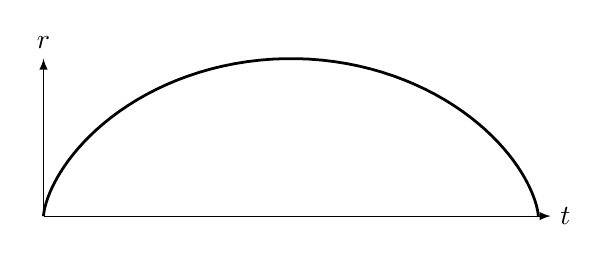
\begin{tikzpicture}
  \coordinate (O) at (0,0);
  \coordinate (A) at (0,2);
  \def\r{20} % radius
  \def\c{3} % center
  \coordinate (C) at (\c, \r);


  \draw[-latex] (O) -- (A) node[anchor=south] {$r$};
  \draw[-latex] (O) -- (2.05*pi,0) node[anchor=west] {$t$};
  \draw[black,domain=0:2*pi,samples=80, line width=1] 
       plot ({\x - sin(\x r)},{1 - cos(\x r)});
  \end{tikzpicture}
\end{center}
  
What goes up, must come down! This curve, which I haven't drawn too well, is just a cycloid, which is the curve traced out by a point on the rim of rolling wheel. So, succumbing to romanticism momentarily we could call this picture ONE TURN OF THE GREAT WHEEL OF TIME.... But there is no reason to expect further turns, because the differential equation simply becomes singular when $r = 0$. We may either say it doesn't make sense to speak of ``before the big bang" or ``after the big crunch" - or we can look for improved laws that avoid these singularities. (I should repeat that we are dealing with unrealistic models here, since for example there is no evidence that there is enough matter around to ``close the universe" and make this solution qualitatively valid - it may well be that there's a big bang but no big crunch. In this case, there's only one singularity to worry about, not two.)

People have certainly not been too ashamed to study the quantum theory of this system (and souped-up variants) in an effort to get a little insight into quantum gravity. We would expect that quantum effects wouldn't matter much until the radius of the universe is very small, but when it is very small they would matter a lot, and maybe - one might hope - they would save the day, preventing the nasty singularities. I'm not saying they DO - this is hotly debated - but certainly some people hope they do. Of course, serious quantum gravity should take into account the fact that geometry of spacetime has all sorts of wiggles in it -it isn't just a symmetrical sphere. This may make a vast difference in how things work out. (For example, the big crunch would be a lot more exciting if there were lots of black holes around by then.) The technical term for the space of all metrics on space is ``superspace" (sigh), and the toy models one gets by ignoring all but finitely many degrees of freedom are called ``minisuperspace" models.

Let's look at a simple minisuperspace model. The simplest thing to try is to take the classical equations of motion \eqref{eq:2} and try to quantize them just like one would a particle in a potential. This is a delicate business, by the way, because one can't just take some classical equations of motion and quantize them in any routine way. There are lots of methods of quantization, but all of them require a certain amount of case-by-case finesse.

The idea of ``canonical quantization" of a classical system with one degree of freedom - like our big bang model above, where the one degree of freedom is $r$ - is to turn the ``position" (that's $r$) into a multiplication operator and the ``momentum" (often that's something like $r'$, but watch out!) into a differentiation operator, say $-i\hbar \frac{d}{dr}$, so that we get the ``canonical commutation relations"
\[[-i\hbar \frac{d}{dr},r] = -i\hbar\]
We then take the formula for the energy, or Hamiltonian, in terms of position and momentum, and plug in these operators, so that the Hamiltonian becomes an operator. (Here various ``operator-ordering" problems can arise, because the position and momentum commuted in the original classical system but not anymore!) To explain what I mean, why don't I just do it!

So: I said that the formula
\begin{equation}
    (r')^2 - (8\pi/3) \frac{D}{r} = -1
\end{equation}
looks a lot like a formula of the form ``kinetic energy plus potential energy is constant". Of course, we could multiply the whole equation by anything and get a valid equation, so it's not obvious that the ``right'' Hamiltonian is
\[(r')^2 - (8\pi/3) \frac{D}{r}\]
or (adding 1 doesn't hurt)
\[(r')^2 - (8\pi/3) \frac{D}{r} + 1\]

In fact, note that multiplying the Hamiltonian by some function of $r$ just amounts to reparametrizing time, which is perfectly fine in general relativity. In fact, Vilenkin and others before him have decided it's better to multiply the Hamiltonian above by $r^2$. Why? Well, it has to do with figuring out what the right notion of ``momentum" is corresponding to the ``position" $r$. Let's do that. We use the old formula
\[p = \frac{dL}{dq'}\]

relating momentum to the Lagrangian, where for us the position, usually called $q$, is really $r$.

The Lagrangian of general relativity is the ``Ricci scalar" $R$ - a measure of curvature of the metric - and in the present problem it turns out to be
\[R = 6(\frac{r''}{r} + \frac{(r')^2}{r^2})\]
But we are reducing the full field theory problem down to a problem with one degree of freedom, so our Lagrangian should be the above integrated over the 3-sphere, which has volume \[16\pi\frac{r^3}{3}\] giving us \[32\pi (r''r^2 + (r')^2 r)\]

However, the $r''$ is a nuisance, and we only use the integral of the Lagrangian with respect to time (that's the action, which classically is extremized to get the equations of motion), so let's do an integration by parts, or in other words add a total divergence, to get the Lagrangian

Differentiating with respect to $r'$ we get the momentum ``conjugate to $r$", \[p = -64\pi r'r\]
Now I notice that Vilenkin uses as the momentum simply $-r'r$, somehow sweeping the monstrous $64\pi$ under the rug. I have the feeling that this amounts to pushing this factor into the definition of $\hbar$ in the canonical commutation relations. Since I was going to set $\hbar$ to 1 in a minute anyway, this is okay (honest). So let's keep life simple and use
\[p = r'r\]
Okay! Now here's the point, we want to exploit the analogy with good old quantum mechanics, which typically has Hamiltonians containing something like $p^2$. So let's take our preliminary Hamiltonian
\[(r')^2 -(8\pi/3) \frac{D}{r} + 1\]
and multiply it by $r^2$, getting
\[H = p^2 - (8\pi \frac{D}{3})r + r^2\].
Hey, what's this? A harmonic oscillator! (Slightly shifted by the term proportional to $r$.) So the universe is just a harmonic oscillator... I guess that's why they stressed that so much in all my classes!

Actually, despite the fact that we are working with a very simple model of quantum cosmology, it's not quite that simple. First of all, recall our original classical equation, \eqref{eq:3}. This constrained the energy to have a certain value. I.e., we are dealing not with a Hamiltonian in the ordinary sense, but a ``Hamiltonian constraint" - typical of systems with time reparametrization invariance. So our quantized equation says that the ``wavefunction of the universe," $\Psi(r)$, must satisfy
\[H\Psi = 0\]
Also, unlike the ordinary harmonic oscillator we have the requirement that $r > 0$. In other words, we're working with a problem that's like a harmonic oscillator and a ``wall" that keeps $r > 0$. Think of a particle in a potential like this:
%FIGURE THIS PLOT OUT
\begin{center}
  \begin{tikzpicture}
  \coordinate (O) at (0,0);
  \coordinate (A) at (0,2);
  \def\r{20} % radius
  \def\c{3} % center
  \coordinate (C) at (\c, \r);


  \draw[-latex] (O) -- (A) node[anchor=south] {$V(r)$};
  \draw[-latex] (O) -- (2.05*pi,0) node[anchor=west] {$r$};
  \draw[black,domain=0:2*pi,samples=80, line width=1] 
       plot ({\x^2 r});
  \end{tikzpicture}
\end{center}

Here $V(r) = - (8\pi \frac{D}{3})r + r^2$. The minimum of $V$ is at $r = 4\pi \frac{D}{3}$ and the zeroes are at $r = 0$ and $8\pi \frac{D}{3}$. Classically, a particle with zero energy starting at $r = 0$ will roll to the right and make it out to $r = 4\piD\frac{D}{3}$ before rolling back to $r = 0$. This is basically the picture we had in Figure 1, except that we've reparametrized time so we have simple harmonic motion instead of cycloid.
Quantum mechanically, however one must pick boundary conditions at $r = 0$ to make the problem well-defined!

This is where the fur begins to fly!! Hawking and Vilenkin have very different ideas about what the right boundary conditions are. And note that this is not a mere technical issue, since they determine the wavefunction of the universe in this approach! I will not discuss this since Vilenkin does so quite clearly, and if you understand what I have written above you'll be in a decent position to understand him. I will just note that Vilenkin, rather than working with a universe full of ``dust," considers a universe in which the dominant contribution to the stress-energy tensor is the cosmological constant, that is, the negative energy density of a ``false vacuum", which believers in inflation (such as Vilenkin) think powered the exponential growth of the universe at an early stage. So his equations are slightly different from those above (and are only meant to apply to the early history of the universe).

[Let me just interject a question to the experts if I may - since I've written this long article primarily to educate myself. It would seem to me that the equation $H\Psi = 0$ above would only have a normalizable solution if the boundary conditions were fine-tuned! I.e., maybe the equation $H\Psi = 0$ itself determines the boundary conditions! This would be very nice; has anyone thought of this? It seems reasonable because, with typical boundary conditions, the operator $H$ above will have pure point spectrum (only eigenvalues) and it would be rather special for one of them to be 0, allowing a normalizable solution of $H\Psi = 0$. Also, corrections and education of any sort are welcomed. I would love to discuss this with some experts.]

Anyway, suppose we find some boundary conditions and calculate $\Psi$, the ``wavefunction of the universe." (I like repeating that phrase because it sounds so momentous, despite the fact that we are working with a laughably oversimplified toy model.) What then? What are the implications for the man in the street?

Let me get quite vague at this point. Think of the radius of the universe as analogous to a particle moving in the potential of Figure 2. In the current state of affairs classical mechanics is an excellent approximation, so it seems to trace out a classical trajectory. Of course it is really obeying the laws of quantum mechanics, so the trajectory is really a ``wave packet" - technically, we use the WKB approximation to see how the wave packet can seem like a classical trajectory. But near the big bang or big crunch, quantum mechanics matters a lot: there the potential is rapidly varying (in our simple model it just becomes a ``wall") and the wave packet may smear out noticeably. (Think of how when you shoot an electron at a nucleus it bounces off in an unpredictable direction - it's wavefunction just tells you the probability that it'll go this way or that!) So some quantum cosmologists have suggested that if there is a big crunch, the universe will pop back out in a highly unpredictable, random kind of way!

I should note that Vilenkin has a very different picture. Since this stuff makes large numbers of assumptions with very little supporting evidence, it is science that's just on the brink of being mythology. Still, it's very interesting.
\find{\paper{Lee Smolin, Finite, diffeomorphism invariant observables in quantum gravity, available as \href{https://arxiv.org/abs/gr-qc/9302011}{gr-qc/9302011.}}}
The big problem in canonical quantization of gravity, once one gets beyond ``mini-" and ``minisuperspace" models, is to find enough diffeomorphism-invariant observables. There is a certain amount of argument about this stuff, and various approaches, but one common viewpoint is that the ``physical" observables, that is, the really observable observables, in general relativity are those that are invariant under all diffeomorphisms of spacetime. I.e., those that are independent of any choice of coordinates. For example, saying ``My position is (242,2361,12,-17)" is not diffeomorphism-invariant, but saying ``I'm having the time of my life" is. It's hard to find lots of (tractable) diffeomorphism invariant observables - or even any! Try figuring out how you would precisely describe the shape of a rock without introducing any coordinates, and you'll begin to see the problem. (The quantum mechanical aspects make it harder.)

Rovelli came up a while back with a very clever angle on this problem. It's rather artificial but still a big start. Using a ``field of clocks" he was able to come up with interesting diffeomorphism invariant observables. The idea is simply that if you had clocks all around you could say ``when the bells rang 2 a.m. I was having the time of my life" - and this would be a diffeomorphism-invariant statement, since rather than referring to an abstract coordinate system it expresses the coincidence of two physical occurences, just like ``the baseball broke through the window". Then he pushed this idea to define ``evolving constants of motion" - a deliberate oxymoron - to deal with the famous ``problem of time" in general relativity: how to treat time evolution in a coordinate-free manner on a spacetime that's not flat and, worse, whose geometry is ``uncertain" a la Heisenberg? This is treated, by the way, in

\find{\paper{Carlo Rovelli, Time in quantum gravity: an hypothesis, Phys. Rev. D43 (1991), 442-456.}}
Also, an excellent and very thorough review of the problem of time and various proposed solutions, including Rovelli's, is given in
\find{\paper{Chris J. Isham, Canonical quantum gravity and the problem of time, 125 pages, available as \href{https://arxiv.org/abs/gr-qc/9210011}{gr-qc/9210011.}}}

Anyway, in a paper I very briefly described in {\hyperref[week1]{week1.tex}}

\find{\paper{Lee Smolin, Time, measurement and information loss in quantum cosmology, available as \href{https://arxiv.org/abs/gr-qc/9301016}{gr-qc/9301016}}}

Smolin showed, how, using a clever trick sketched in the present paper to get ``observables" invariant under spatial but not temporal observables, together with Rovelli's idea, one could define lots of REAL observables, invariant under spacetime diffeomorphisms that is, thus making a serious bite into this problem.

I warn the reader that there is a fair amount that is not too realistic about these methods. First there's the ``clock field" - this can actually be taken as a free massless scalar field, but in so doing there is the likelihood of serious technical problems. Some of these are discussed in
\find{\paper{P. Hajicek, Comment on ``Time in quantum gravity - an hypothesis", Phys. Rev. D44 (1991), 1337-1338.}}
(But I haven't actually read this, just Isham's description.) Also, the clever trick of the present paper is to couple gravity to an antisymmetric tensor gauge field so that in addition to having loops as part of ones "loop representation," one has surfaces - a ``surface representation". But this antisymmetric tensor gauge field is not the sort of thing that actually seems to arise in physics (unless I'm missing something). Still, it's a start. I think I'll finish by quoting Smolin's abstract:
\begin{quote}
    Two sets of spatially diffeomorphism invariant operators are constructed in the loop representation formulation of quantum gravity. This is done by coupling general relativity to an anti- symmetric tensor gauge field and using that field to pick out sets of surfaces, with boundaries, in the spatial three manifold. The two sets of observables then measure the areas of these surfaces and the Wilson loops for the self-dual connection around their boundaries. The operators that represent these observables are finite and background independent when constructed through a proper regularization procedure. Furthermore, the spectra of the area operators are discrete so that the possible values that one can obtain by a measurement of the area of a physical surface in quantum gravity are valued in a discrete set that includes integral multiples of half the Planck area. These results make possible the construction of a correspondence between any three geometry whose curvature is small in Planck units and a diffeomorphism invariant state of the gravitational and matter fields. This correspondence relies on the approximation of the classical geometry by a piecewise flat Regge manifold, which is then put in correspondence with a diffeomorphism invariant state of the gravity-matter system in which the matter fields specify the faces of the triangulation and the gravitational field is in an eigenstate of the operators that measure their areas.
\end{quote}



\week{February 20, 1993}

%\week{March 1, 1993}
\find{\paper{Mathematical problems of non-perturbative quantum general relativity (lectures delivered at the 1992 Les Houches summer school on Gravitation and Quantization), by Abhay Ashtekar, 87 pp, Plain TeX, available as {\href{https://arxiv.org/abs/gr-qc/9302024}{arXiv:gr-qc/9302024}.}}}

I described this paper in {\hyperref[week3]{week3.tex}}, but now it's available from gr-qc. It's a good quick introduction to the loop representation of quantum gravity.

\find{\paper{Lectures on Non-perturbative Canonical Gravity, by Abhay Ashtekar, World Scientific Press, 1991.}}

This book, which I finally obtained, is the introduction to the loop representation of quantum gravity. What's the loop representation? Well, this is a long story, so you really should read the book. But just to get you going, let me describe Ashtekar's "new variables," which form the basis for Rovelli and Smolin's construction of the loop representation.

First, recall that general relativity is usually thought of as a theory about a metric on spacetime - more precisely, a Lorentzian metric. Here spacetime is a 4-dimensional manifold, and a Lorentzian metric allows you to calculate the "dot product" of any two tangent vectors at a point. This is in quotes because, while a normal dot product might look like.

\[(v_0,v_1,v_2,v_3) \cdot (w_0,w_1,w_2,w_3) =  v_0w_0 + v_1w_1 + v_2w_2 + v_3w_3\]
relative to some basis, for a Lorentzian metric we can always find a basis of the tangent space such that
\[(v_0,v_1,v_2,v_3)\cdot (w_0,w_1,w_2,w_3) = v_0w_0 - v_1w_1 - v_2w_2 - v_3w_3\]

Now the metric in general relativity defines a "connection," which tells you a tangent vector might "twist around" as you parallel translate it, that is, move it along while trying to keep it from rotating unnecessarily. Here "twist around" is in quotes because, since you are parallel translating the vector, it's not really "twisting around" in the usual sense, but it might seem that way relative to some coordinate system. For example, if you used polar coordinates to describe parallel translation on the plane, it might seem that the unit vector in the r direction "twisted around" towards the $\theta$ direction as you dragged it along. But in another coordinate system - say the usual $x-y$ system - it would not appear to be "twisting around". This fact is expressed by saying "the connection is not a tensor".

But from the connection we can cook up a big fat tensor, the "Riemann tensor" $R^i_{jkl}$, which says how much the vector in the lth direction (here the indices range from 0 to 3) twists towards the ith direction when you move it around a teeny little square in the j-k plane. The Lagrangian in ordinary GR is just the integral of the "Ricci scalar curvature," R, which is gotten from the Riemann tensor by "contraction", i.e. summing over the indices in a certain way:

\[R = R^i_{ji}^j\]

Where we are raising indices using the metric in a manner beloved by physicists and feared by many mathematicians. If you integrate the Lagrangian over a region of spacetime you get the "action", and in classical general relativity (in a vacuum, for simplicity) one can formulate the laws of motion simply by saying: any teeny change in the metric that vanishes on the boundary of the region should leave the action constant to first order. In other words, the solutions of the equations of general relativity are the *stationary points* of the action. If you know how to do variational calculus you can derive Einstein's equations from this variational principle, as it's called. Mathematicians will be pleased to know that Hilbert beat Einstein to the punch here, so the integral of R is called the "Einstein-Hilbert" action for general relativity.

But there's another formulation of general relativity in terms of an action principle. This is called the "Palatini" action - and actually I'm going to describe a slight variation on it, that is conceptually simpler, and apparently appears for the first time in Ashtekar's book. The Palatini approach turns out to be more elegant and is a nice stepping-stone to the Ashtekar approach. In the Palatini approach one thinks of general relativity not as being a theory of a metric, but of a "tetrad" and an "$\mathfrak{so(3,1)}$ connection". To explain what these are, I will cut corners and assume all the fiber bundles lurking around are trivial; the experts will easily be able to figure out the general case. So: an (orthonormal) tetrad, or "vierbein," is a just a kind of field on spacetime which at each point consists of an (ordered) orthonormal basis of the tangent space. If we express the metric in terms of a tetrad, it looks just like the formula for the standard "inner product"
\[(v_0,v_1,v_2,v_3)\cdot(w_0,w_1,w_2,w_3) = v_0w_0 - v_1w_1 - v_2w_2 - v_3w_3\]
This allows us to identify the group of linear transformations of the tangent space that preserve the metric with the group of linear transfomations preserving the standard "inner product," which is called $SO(1,3)$ since there's one plus sign and three minuses. And from the connection mentioned above one gets an $SO(1,3)$ connection, or, what's more or less the same thing, an so (1,3)-valued 1-form, that is, a kind of field that can eat a tangent vector at any point and spits out element of the Lie algebra $\mathfrak{so}(1,3)$.

What's $\mathfrak{so}(1,3)$? Well, elements of $\mathfrak{so(1,3)}$ include "infinitesimal" rotations and Lorentz transformations, since $SO(1,3)$ is generated by rotations and Lorentz transformations. More precisely, $\mathfrak{so(1,3)}$ is a 6-dimensional Lie algebra having as a basis the three infinitesimal rotations $J_1, J_2$, and $J_3$ around the three axes, and the three infinitesimal Lorentz transformations or "boosts" $K_1, K_2, K_3$. The bracket in this most important Lie algebra is given by\\
$[J_i,J_j] = J_k$\\
$[K_i,K_j] = -J_k$\\
$[J_i,K_j] = K_k$\\
where $(i,j,k)$ is a cyclic permutation (1,2,3). (I hope I haven't screwed up the signs.) Note that the $J$'s by themselves form a Lie subalgebra called $\mathfrak{so}(3)$, the Lie algebra of the rotation group $SO(3)$. Note that $\mathfrak{so}(3)$ is isomorphic to the the cute little Lie algebra $\mathfrak{su}(3)$ I described in my post {\hyperref[week5]{week5.tex}}; $J_1, J_2$, and $J_3$ correspond to the guys $I, J$, and $K$ divided by two.

The $\mathfrak{so(1,3)}$ connection has a curvature, and using the tetrads again we can identify this with the Riemann curvature tensor. So the Palatini trick is to rewrite the Einstein-Hilbert action in terms of the curvature of the $\mathfrak{so(1,3)}$ connection and the tetrad field. This is called the Palatini action. Charmingly, even though the tetrad field is utterly unphysical, we can treat it and the $\mathfrak{so(1,3)}$ connection as independent fields and, doing calculus of variations to find stationary points of the action, we get equations equivalent to Einstein's equations.

Ashtekar's "new variables" - from this point of view - rely on a curious and profound fact about $\mathfrak{so(1,3)}$. Note that $\mathfrak{so(1,3)}$ is a Lie algebra over the real numbers. But if we allow ourselves to form complex linear combinations of the $J$'s and $K$'s, thus:
\\
$M_i = \frac{(J_i + iK_i)}{2}$\\
$N_i = \frac{(J_i - iK_i)}{2}$\\
(please don't mix up the subscript $i = 1,2,3$ with the other $i$, the square root of minus one) we get the following brackets:

\\
$[M_i,M_j] = M_k$\\
$[N_i,N_j] = N_k$\\
$[M_i,N_j] = 0$\\
I think the signs all work but I wouldn't trust me if I were you. The wonderful thing here is that the $M$'s and $N$'s commute with each other, and each set has commutation relations just like the $J$'s! The $J$'s, recall, are infinitesimal rotations, and the Lie algebra they span is $\mathfrak{so}(3)$. So in a sense the Lie algebra of the Lorentz group can be "split" into "left-handed" and "right-handed" copies of $\mathfrak{so}(3)$, also known as "self-dual" and "anti-self-dual" copies. This is, in fact, what lies behind the handedness of neutrinos, and many other wonderful things.

But let me phrase this result more precisely. Since we allowed ourselves complex linear combinations of the J's and K's, we are now working in the "complexification" of the Lie algebra $\mathfrak{so}(3,1)$, and we have shown that this Lie algebra over the complex numbers splits into two copies of $\mathfrak{so}(3,\C)$, the complexification of $\mathfrak{so}(3)$.

Ashtekar came up with some "new variables" for general relativity in the context of the Hamiltonian approach. Here we are working in the Lagrangian approach, where things are simpler because they are "generally covariant," not requiring a split of spacetime into space and time. The Lagrangian approach to the new variables is due to Samuel, Jacobson and Smolin, and in this approach all they amount to is this: $\mathfrak{so}(1,3)$ connection of the Palatini approach, think of the$\mathfrak{so}(1,3)$ as sitting inside the complexification thereof, and consider only the "right-handed" part! Thus, from an $\mathfrak{so}(1,3)$ connection, we get a $\mathfrak{so}(3,\C)$ connection. The "new variables" are just the tetrad field and this $\mathfrak{so}(3,\C)$ connection.

I have tried to keep down the indices but I think I will write down the Palatini Lagrangian and then the "new variables" Lagrangian, without explaining exactly what they mean, just to show how amazingly similar-looking they are. In the Palatini approach we have a tetrad field, which now we write in its full glory as $e_I^i$, and the curvature of the $\mathfrak{so}(1,3)$ connection, which now we write as $\Omega_{ij}^{IJ}$. The Lagrangian is then
$e_I^i e_J^j \Omega_{ij}^{IJ}$
(which we integrate against the usual volume form to get the action). In the new variables approach we have a tetrad field again, and we write the curvature of the $\mathfrak{so}(3,\C)$  connection as $F_{ij}^{IJ}$. (This turns out to be just the "right-handed" part of  $\Omega_{ij}^{IJ}$.) The Lagrangian is
$e_I^i e_J^j F_{ij}^{IJ}$ !

Miraculously, this also gives Einstein's equations.

What's utterly unclear from what I've said so far is why this helps so much in trying to quantize gravity. I may eventually get around to writing about that, but for now, read the book!

\find{\paper{We are not stuck with gluing, by David Yetter and Louis Crane, preprint available as {\href{https://arxiv.org/abs/hep-th/9302118}{arXiv:hep-th/9302118}.}}}

Well, in {\hyperref[week2]{week2.tex}} I mentioned Crane and Yetter's marvelous construction of a 4d topological quantum field theory using the representations of the quantum group $SU_q(2)$ - and in {\hyperref[week5]{week5.tex}} I mentioned Ocneanu's "proof" that the resulting 4-manifold invariants were utterly trivial (equal to 1 for all 4-manifolds). Now Crane and Yetter have replied, saying that their 4-manifold invariants are not trivial and that Ocneanu interpreted their paper incorrectly. I look forward to the conference on quantum topology in Kansas at the end of May, where the full story will doubtless come out.
\\
\find{\paper{The initial value problem in light of Ashtekar's variables, by R. Capovilla, J. Dell and T. Jacobson, preprint available as {\href{https://arxiv.org/abs/gr-qc/9302020}{{arxiv:gr-qc/9302020}},15 pages.}}}
The advantage of Ashtekar's new variables is that the simplify the form of the constraint equations one gets in the initial-value problem for general relativity. This is true both of the classical and quantum theories. Rovelli and Smolin used this to find, for the first time, lots of states of quantum gravity defined by link invariants. Here the above authors are trying to apply the new variables to the \textit{classical} theory.

\find{\paper{Combinatorial expression for universal Vassiliev link invariant, by Sergey Piunikhin, preprint available as {\href{https://arxiv.org/abs/hep-th/9302084}{{arxiv:hep-th/9302084}}.}}}
Somebody ought to teach those Russians how to use the word "the" now that the cold war is over. Anyway, this paper defines a kind of universal object for Vassiliev invariants, which is sort of similar to what I was trying to do in

\find{\paper{Link invariants of finite type and perturbation theory, by John Baez, Lett. Math. Phys. 26 (1992) 43-51.}}

but more concrete, and (supposedly) simpler than Kontsevich's approach. My parenthesis simply indicates that I haven't had time to figure out what's going on here.



\week{March 1, 1993}

%\week{March 5, 1993}
I was delighted to find that Louis Kauffman wants to speak at the workshop at UCR on knots and quantum gravity; he'll be talking on "Temperley Lieb recoupling theory and quantum invariants of links and manifolds". His books

On knots, by Louis H. Kauffman, Princeton, N.J., Princeton University Press, 1987 (Annals of Mathematics Studies, no. 115)

and more recently

Knots and physics, by Louis H. Kauffman, Teaneck, NJ, World Scientific Press, 1991 (K & E Series on Knots and Everything, vol. 1)

are a lot of fun to read, and convinced me to turn my energies towards the intersection of knot theory and mathematical physics. As you can see by the title of the series he's editing, he is a true believer the deep significance of knot theory. This was true even before the Jones polynomial hit the mathematical physics scene, so he was well-placed to discover the relationship between the Jones polynomial (and other new knot invariants) and statistical mechanics, which seems to be what won him his fame. He is now the editor of a journal, "Journal of knot theory and its ramifications."

He sent me a packet of articles and preprints which I will briefly discuss. If you read any of the stuff below, please read the delightful reformulation of the 4-color theorem in terms of cross products that he discovered! I am strongly tempted to assign it to my linear algebra class for homework....

\find{\paper{Map coloring and the vector cross product, by Louis Kauffman, J. Comb. Theory B, 48 (1990) 45.}}

Map coloring, 1-deformed spin networks, and Turaev-Viro invariants for 3-manifolds, by Louis Kauffman, Int. Jour. of Mod. Phys. B, 6 (1992) 1765-1794.

An algebraic approach to the planar colouring problem, by Louis Kauffman and H. Saleur, in Comm. Math. Phys. 152 (1993), 565-590.

As we all know, the usual cross product of vectors in $R^3$ is not associative, so the following theorem is slightly interesting:

Theorem: Consider any two bracketings of a product of any finite number of vectors, e.g.: 
\[L = a \times (b \times ((c \times d) \times e)  \quad and \quad  R = ((a \times b) \times c) \times (d \times e)\]

Let $i,j,k$ be the usual canonical basis for $R^3$:
\[i = (1,0,0) \quad j = (0,1,0) \quad k = (0,0,1)\].

Then we may assign $a,b,c,...$ values taken from ${i,j,k}$ in such a way that $L = R$ and both are nonzero.

But what's really interesting is:

Meta-Theorem: The above proposition is equivalent to the 4-color theorem. Recall that this theorem says that any map on the plane may be colored with 4 colors in such a way that no two regions with the same color share a border (an edge).

What I mean here is that the only way known to prove this Theorem is to deduce it from the 4-color theorem, and conversely, any proof of this Theorem would easily give a proof of the 4-color theorem! As you all probably know, the 4-color theorem was a difficult conjecture that resisted proof for about a century before succumbing to a computer-based proof require the consideration of many, many special cases:

Every planar map is four colorable, by K. I. Appel and W. Haken, Bull. Amer. Math. Soc. 82 (1976) 711.

So the Theorem above may be regarded as a profoundly subtle result about the "associativity" of the cross product!

Of course, I hope you all rush out now and find out how this Theorem is equivalent to the 4-color theorem. For starters, let me note that it uses a result of Tait: first, to prove the 4-color theorem it's enough to prove it for maps where only 3 countries meet at each vertex (since one can stick in a little new country at each vertex), and second, 4-coloring such a map is equivalent to coloring the edges with 3 colors in such a way that each vertex has edges of all 3 colors adjoining it. The 3 colors correspond to $i, j$, and $k$!

Kauffman and Saleur (the latter a physicist) come up with another algebraic formulation of the 4-color theorem in terms of the Temperley-Lieb algebra. The Temperley-Lieb algebra $TL_n$ is a cute algebra with generators $e_1, ..., e_{n-1}$ and relations that depend on a constant d called the "loop value":\\
$e_i^2 = de_i$\\
$e_i e_{i+1} e_i = e_i$\\
$e_i e_{i-1} e_i = e_i$\\
$e_i e_j = e_j e_i$     for $|i -j| > 1$.
The point of it becomes clear if we draw the $e_i$ as tangles on $n$ strands. Let's take $n=3$ to keep life simple. Then $e_1$ is\\

\begin{verbatim}
\  /   |
 \/    |
       |
 /\    |
/  \   |

\end{verbatim}
while $e_2$ is
\begin{verbatim}
|   \  /  
|    \/   
|      
|    /\   
|   /  \  

\end{verbatim}
In general, $e_i$ "folds over" the ith and (i+1)st strands. Note that if we square $e_i$ we get a loop - e.g., $e_1$ squared is
\begin{verbatim}
\  /   |
 \/    |
       |
 /\    |
/  \   |
\  /   |
 \/    |
       |
 /\    |
/  \   |
\end{verbatim}
Here we are using the usual product of tangles (see the article "tangles" in the collection of my expository posts, which can be obtained in a manner described at the end of this post). Now the rule in Temperley-Lieb land is that we can get rid of a loop if we multiply by the loop value d; that is, the loop "equals" $d$. So $e_1$ squared is just $d$ times 
\begin{verbatim}
\  /   |
 \/    |
       |
       |
       |
       |
       |
       |
 /\    |
/  \   |

\end{verbatim}

which - since we are doing topology - is the same as $e_1$. That's why $e_i^2$ = $de_i$.

The other relations are even more obvious. For example, $e_1$ $e_2$ $e_1$ is just \\
\\
\\
\\

\begin{verbatim}
\  /   |
 \/    |
       |
 /\    |
/  \   |
|   \  /  
|    \/   
|      
|    /\   
|   /  \  
\  /   |
 \/    |
       |
 /\    |
/  \   |
\end{verbatim}
which, since we are doing topology, is just $e_1$! Similarly, $e_2 e_1 e_2 = e_1$, and $e_i$ and $e_j$ commute if they are far enough away to keep from running into each other.

As an exercise for combinatorists: figure out the dimension of $TL_n$.

Okay, very cute, one might say, but so what? Well, this algebra was actually first discovered in statistical mechanics, when Temperley and Lieb were solving a 2-dimensional problem:

Relations between the `percolation' and `coloring' problem and other graph-theoretical problems associated with tregular planar lattices: some exact results on the `percolation' problem, by H. N. V. Temperley and E. H. Lieb, Proc. Roy. Soc. Lond. A 322 (1971), 251 - 280.

It gained a lot more fame when it appeared as the explanation for the Jones polynomial invariant of knots - although Jones had been using it not for knot theory, but in the study of von Neumann algebras, and the Jones polynomial was just an unexpected spinoff. Its importance in knot theory comes from the fact that it is a quotient of the group algebra of the braid group (as explained in "Knots and Physics"). It has also found a lot of other applications; for example, I've used it in my paper on quantum gravity and the algebra of tangles. So it is nice to see that there is also a formulation of the 4-color theorem in terms of the Temperley-Lieb algebra (which I won't present here).

\find{\paper{Knots and physics, by Louis Kauffman, Proc. Symp. Appl. Math. 45 (1992), 131-246.}}

Spin networks, topology and discrete physics, by Louis Kauffman, University of Illinois at Chicago preprint.

Vassiliev invariants and the Jones polynomial, by Louis Kauffman, University of Illinois at Chicago preprint.

Gauss codes and quantum groups, by Louis Kauffman, University of Illinois at Chicago preprint.

Fermions and link invariants, by Louis Kauffman and H. Saleur, Yale University preprint YCTP-P21-91, July 5, 1991.

State models for link polynomials, by Louis Kauffman, L'Enseignement Mathematique, 36 (1990), 1 - 37.

The Conway polynomial in $R^3$ and in thickened surfaces: a new determinant formulation, by F. Jaeger, Louis Kauffman and H. Saleur, preprint.

These are a variety of papers on knots, physics and everything.... The more free-wheeling among you might enjoy the comments at the end of the first paper on "knot epistemology."

I am going to a conference on gravity at UC Santa Barbara on Friday and Saturday, which I why I am posting this early, and why I have no time to describe the above papers. I'll talk about my usual obsessions, and hear what other people are up to, perhaps bringing back some words of wisdom for next week's "This Week's Finds". 
\week{March 5, 1993}

\week{March 12, 1993}

\find{\paper{Surgical invariants of four-manifolds, by Boguslaw Broda, preprint available as {\href{https://arxiv.org/abs/hep-th/9302092}{arxiv:hep-th/9302092}.}}}

There a number of attempts underway to get invariants of four-dimensional manifolds (and 4d topological quantum field theories) by techniques analogous to those that worked in three dimensions. The 3-manifold invariants and 3d topological quantum field theories got going with the work of Witten on Chern-Simons theory, but since this was not rigorous a number of ways were devised to make it so. These seem different at first glance but all give the same answer. Two approaches that use a lot of category theory are the Heegard splitting approach (due to Crane, Kohno and Kontsevich, in which one writes a 3-manifold as two solid n-holed tori glued together by a diffeomorphism of their boundaries), and the surgery on links approach (due to Reshetikhin and Turaev, in which one builds up 3-manifolds by starting with the 3-sphere, cutting out thickened links and gluing them back in a different way, allowing one to define invariants of 3-manifolds from link invariants). In the case of 3 dimensions a nice paper relating the Heegard splitting and the surgery on links approaches is

Reshetikhin-Turaev and Crane-Kohno-Kontsevich 3-manifold invariants coincide, by Sergey Piunikhin, preprint, 1992. (Piunikhin is at serguei@math.harvard.edu.)

People are now trying to generalize all these ideas to 4-manifolds. There is already an interesting bunch of 4-manifold invariants out there, the Donaldson invariants, which are hard to compute, but were shown (heuristically) by Witten to be related to a quantum field theory. Lately people have been trying to define invariants using category theory; these may or may not turn out to be the same.

I've already been trying to keep you all updated on the story about Crane and Yetter's 4d TQFT. This week I'll discuss another approach, with a vast amount of help from Daniel Ruberman, a topologist at Brandeis. Any errors in what I write on this are likely to be due to my misunderstandings of what he said - caveat emptor! Broda's paper is quite terse - probably due to the race that is going on - and is based on:

A link calculus for 4-manifolds, by E. Cesar de Sa, in Topology of Low-Dimensional Manifolds, Proc. Second Sussex Conf., Lecture Notes in Math., vol. 722, Springer, Berlin, 1979, pp. 16-30.

so I should start by describing what little I understand of de Sa's work.

One can describe (compact, smooth) 4-manifolds in terms of handlebody decomposition. This allows one to actually draw pictures representing 4-manifolds. A lot of times when people first hear about topology they get they impression that it's all about rubber doughnuts, Mobius strips, and other Dali-esque wiggly objects in hyperspace. Then, when they take courses in it, they are confronted with nasty separation axioms and cohomology theories! This is just to scare away outsiders! Handlebody theory really is about wiggly objects in hyperspace, and it's lots of fun - though to be good in it you need to know your point set topology and your algebraic topology, I'm afraid - and much better than I do!
\\
Recall: 
\\
$D^n$ = unit ball in $R^n$\\
$S^n$ = unit sphere in $R^{n+1}$\\
\\
In particular note that $S^0$ is just two points. Note that:
\\
the boundary of $D^4$ is $S^3$\\
the boundary of $D^3 \times D^1$ is $D^3 \times S^0 \bigcap S^2 \times D^1$\\
the boundary of $D^2 \times D^2$ is $D^2 \times S^1 \bigcap S^1 \times D^2$\\
the boundary of $D^1 \times D^3$ is $D^1 \times S^2 \bigcap S^0 \times D^3$\\
the boundary of $D^4$ is $S^3$\\

I have written this rather redundant chart in a way that makes the pattern very clear and will come in handy below for those who aren't used to this stuff.

To build up a 4-manifold we can start with a "0-handle," $D^4$, which has as boundary $S^3$.

Then we glue on "1-handles," that is, copies of $D^3 \times D^1$. Note that part of the boundary of $D^1 \times D^3$ is $D^3 \times S^0$, which is two $D^3$'s; when we glue on a 1-handle we simply attach these two $D^3$'s to the $S^3$ by a diffeomorphism. The resulting space is not really a smooth manifold, but it can be smoothed. It then becomes a smooth 4-manifold with boundary.

Then we glue on "2-handles" by attaching copies of $D^2 \times D^2$ along the part of their boundary that is $D^2 \times S^1$. Then we smooth things out.

Then we glue on "3-handles" by attaching copies of $D^1 \times D^3$ along the part of their boundary that is $D^1 \times S^2$. Then we smooth things out.

Then we glue on "4-handles" by attaching copies of $D^4$ along their boundary, i.e. $S^3$.

We can get any compact oriented 4-manifold this way using attaching maps that are compatible with the orientations. The reader who is new to this may enjoy constructing 2-manifolds in an analogous way. Compact oriented 2-manifolds with boundary are just n-holed tori.

What's cool is that with some tricks one can still draw what's going in the case of 3-manifolds and 4-manifolds. Here I'll just describe how it goes for 4-manifolds, since that's what Cesar de Sa and Broda are thinking about. By the way, a good introduction to this stuff is

The Topology of 4-manifolds, by Robion C. Kirby, Springer-Verlag Lecture Notes in Mathematics (1989), vol. 1374.

So - here is how we draw what's going on. I apologize for being somewhat sketchy here (sorry for the pun, too). I am a bit rushed since I'm heading off somewhere else next weekend... and I am not as familiar with this stuff as I should be.

So, when we start with our 0-handle, or $D^4$, we "draw" its boundary, $S^3$. Think of $S^3$ as $R^3$ and a point at infinity. Since we use perspective when drawing pictures of 3-d objects, this boils down to pretending that our blackboard is a picture of $S^3$!

As we add handles we continue to "draw" what's happening at the boundary of the 4-manifold we have at each stage of the game. 1-handles are attached by gluing a $D^3 \times D^1$ onto the boundary along two $D^3$'s - or balls - so we can just draw the two balls.

2-handles are attached by gluing a $D^2 \times D^2$ onto the boundary of the 4-manifold we have so far along a $D^2 \times S^1$ - or solid torus, so we just need to figure out how to draw an embedded solid torus. Well, for this we just need to draw a knot (that is, an embedded circle), and write an integer next to it saying how many times the embedded solid torus "twists" - plus or minus depending on clockwise or counterclockwise - as we go around the circle. In other words, an embedded solid torus is (up to diffeomorphism) essentially the same as a framed knot. If we are attaching a bunch of 2-handles we need to draw a framed link.

Things get a bit hairy in the case when one of the framed links goes through one of the 1-handles that we've already added. It's easier to draw this situation if we resort to another method of drawing the 1-handles. It's a bit more subtle, and took me quite a while to be able to visualize (unfortunately I seem to have to visualize this stuff to believe it). So let's go back to the situation where we have $D^4$ $S^3$ as its boundary, and we are adding 1-handles. Instead of drawing two balls, we draw an unknotted circle with a dot on it! The dot is just to distinguish this kind of circle from the framed links we already have. But what the circle means is this. The circle is the boundary of an obvious $D^2$, and we can push the interior of this $D^2$ (which is sitting in the $S^3$) into the interior of $D^4$. If we then remove a neighborhood of the $D^2$, what we have left is $S^1 \times D^3$, which is just the result of adding a 1-handle to $D^4$.

This is probably easier to visualize one dimension down: if we have a good old unit ball, $D^3$, and slap an interval, or $D^1$, onto its boundary, and then push the interior of the interval into the interior of the ball, and remove a neighborhood of the interval, what we have left is just an $S^1 \times D^2$.

So in short, we can draw all the 1-handles by drawing unlinked, unknotted circles with dots on them, and then draw all the 2-handles by drawing framed links that don't intersect these circles.

At this point, if you have never seen this before, you are probably dreading the 3-handles and 4-handles. Luckily a theorem comes to our rescue! If we start at the other end of our handlebody decomposition, as it were, we start with 4-handles and glue on 3-handles. If you ponder the chart and see what the pattern of what we're doing is, you'll see that a single 4-handle with some 3-handles stuck on is just the same as a 0-handle with some 1-handles stuck on. So when we now glue this thing (or things) onto the stuff we've built out of 0-, 1-, and 2-handles, we are doing so using a diffeomorphism of its boundary. But a theorem of Laudenbach and Poenaru,

A note on 4-dimensional handlebodies, by F. Laudenbach and V. Poenaru, Bull. Math. Soc. France 100 (1972), pp. 337-344,

says that any such diffeomorphism extends to one of the interior. This means that it doesn't make a darn bit of difference which diffeomorphism we use to glue it on. In short, all the information is contained in the 1- and 2-handles, so we can draw 4-manifolds by first drawing a batch of unknotted unlinked circles with dots on them and then drawing a framed link in the complement.

[A question for the experts, since I'm just learning this stuff: in the above we seem to be assuming that there's only one 0-handle. Is this an okay assumption or do we need something fancier if there's more?]

Now a given 4-manifold may have lots of different handlebody decompositions. So, as usual, we would like to have a finite set of "moves" that allow us to get between any pair of handlebody decompositions of the same 4-manifold. Then we can construct a 4-manifold invariant by cooking up a number from a handlebody decomposition - presented as a picture as above, if we want - and showing that it doesn't change under these "moves".

So, what de Sa did was precisely to find such a set of moves. (There, that's what I understand of his work!)

And what Broda did was precisely to use the Kauffman bracket invariant of framed links to cook up an invariant of 4-manifolds from the handlebody decomposition - which, note, involves lots of links. Recall that the Kauffman bracket assigns to each link a polynomial in one variable, $q$. Here "$q$" is just the same $q$ that appears in the quantum group $SU_q(2)$. As I mentioned in {\hyperref[week5]{week5.tex}} this acts quite differently when $q$ is a root of unity, and the 3d topological quantum field theories coming from quantum groups, as well as Crane and Yetter's 4d topological quantum field theory, come from considering this root-of-unity case. So it's no surprise that Broda requires $q$ to be a root of unity.

Ruberman had some other remarks about Broda's invariant, but I think I would prefer to wait until I understand them....

\find{\paper{Minisuperspaces: symmetries and quantization, by Abhay Ashtekar, Ranjeet S. Tate and Claes Uggla Syracuse University preprint SU-GP-92/2-5, 14 pages, available in latex form as \href{https://arxiv.org/abs/gr-qc/9302026}{gr-qc/9302026}.}}

Minisuperspaces: observables and quantization, Abhay Ashtekar, Ranjeet S. Tate and Claes Uggla Syracuse University preprint SU-GP-92/2-6, 34 pages, available in latex form as \href{https://arxiv.org/abs/gr-qc/9302027}{gr-qc/9302026}

I was just at the Pacific Coast Gravity Meeting last weekend and heard Ranjeet Tate talk on this work. Recall first of all that minisuperspaces are finite-dimensional approximations to the phase space of general relativity, and are used to get some insight into quantum gravity. I went through an example in {\hyperref[week6]{week6.tex}}. In these papers, the authors quantize various "Bianchi type" minisuperspace models. The "Bianchi type" business comes from a standard classification of homogeneous (but not necessarily isotropic) cosmologies and having a lot of symmetry. It is based in part on Bianchi's classification of 3-dimensional Lie algebras into nine types. The second paper gives a pretty good review of this stuff before diving into the quantization, and I should learn it!

The most exciting aspect of these papers, at least to the dilettante such as myself, is that one can quantize these models and show that quantization does NOT typically remove the singularities ("big bang" and/or "big crunch"). Of course, these models have only finitely many degrees of freedom, and are only a caricature of full-fledged quantum gravity, so one can still argue that real quantum gravity will get rid of the singularities. But a number of general relativists are arguing that this is not the case, and we simply have to learn to live with singularities. So it's good to look at models, however simple, where one can work things out in detail, and not just argue about generalities.

\find{\paper{Unique determination of an inner product by adjointness relations in the algebra of quantum observables, by Alan D. Rendall, Max-Planck-Institut fuer Astrophysik preprint.}}

I had known Rendall from his work on the perturbative expansion of the time evolution operators in classical general relativity. He became interested in quantum gravity a while ago and visited Ashtekar and Smolin at Syracuse University, since (as he said) the best way to learn is by doing. There he wrote this paper on Ashtekar's approach to finding the right inner product for the space of states of quantum gravity. I had heard about this paper, but hadn't seen it until I met Rendall at the gravity meeting last weekend. He gave me a copy and explained it. It is a simple and beautiful paper - such nice mathematical results that I am afraid someone else may have found them earlier somewhere.

Ashtekar's idea is to fix the inner product by requiring that the physical observables, which are operators on the space of states, be self-adjoint. Rendall shows the following. Let $A$ be a *-algebra acting on a vector space $V$. Let us say that an inner product on $V$ is "strongly admissable" if 1) the representation is a *-representation with respect to this inner product, 2) for each element of $A$, the corresponding linear transformation on $V$ is bounded relative to the norm given by this inner product, and 3) the completion of $V$ in the inner product is a topologically irreducible representation of $A$. Rendall shows the uniqueness of a strongly admissible inner product on any representation $V$ of $A$ (up to a constant multiple). Of course, such an inner product need not exist, but when it does, it is unique. This is as nice a result along these lines as one could hope for. He also has a more complicated result that applies to unbounded operators. A good piece of work on the foundations of quantum theory!

\find{\paper{Thawing the frozen formalism: the difference between observables and what we observe, by Arlen Anderson, preprint available as}\href{https://arxiv.org/abs/gr-qc/9211028}{gr-qc/9211028}.}


There were a number of youngish folks giving talks at the gravity meeting who have clearly been keeping up with the recent work on the problem of time and other conceptual problems in quantum gravity. In very brief terms, the problem of time is that in general relativity, we have not a Hamiltonian in the traditional sense, but a "Hamiltonian constraint" H = 0, so when we quantize it superficially appears that there are no dynamics whatsoever (as it seems like we have a zero Hamiltonian!). That's the reason for the term "frozen formalism" - and the desire to "thaw" it, or find the dynamics lurking in it. In fact, the Hamiltonian constraint is just a reflection of the fact that general relativity has no preferred time coordinate, and we are just learning how to deal with the quantum theory of such systems. For a good survey of the problem and some new proposed solutions, I again refer everyone to Isham's paper:

\find{\paper{Canonical Quantum Gravity and the Problem of Time, Chris J. Isham, 125 pages of LaTeX output, preprint available as \href{https://arxiv.org/abs/gr-qc/9210011} {gr-qc/9210011}.}}

In particular, one interesting approach is due to Rovelli, and is called "evolving constants of motion" (a deliberate and very accurate oxymoron). While there are serious technical problems with this approach, it's very natural from a physical point of view - at least once you get used to it. I have the feeling that the younger physicists are, as usual, getting used to it a lot more quickly than the older folks who have been pondering the problem of time for many years. Anderson is one of these younger folks, and his paper develops Rovelli's approach in terms of in a toy model, namely the case of two free particles satisfying the Schrodinger equation.

\find{\paper{The extended loop group: an infinite dimensional manifold associated with the loop space, by Cayetano Di Bartolo, Rodolfo Gambini and Jorge Griego, 42 pages, preprint available as \href{https://arxiv.org/abs/gr-qc/9303010}{gr-qc/9303010}.}}

Unfortunately I don't have the time now to give this paper the discussion it deserves. Gambini is one of the original inventors of the loop representation of gauge theories, so his work is especially worth paying attention to. He explained the idea of this paper to me a while back. Its aim is to provide a workable "calculus" for the loop representation by enlarging the ordinary loop group to a larger group which is actually an infinite-dimensional Lie group - the point being that the usual loop group doesn't have a Lie algebra, but this one does. As one might expect, the Lie algebra of this group is closely related to the theory of Vassiliev invariants. The paper considers some applications to quantum gravity and knot theory. 




\week{March 20, 1993}


\week{March 23, 1993}



% ==> week12.tex <==
\week{April 10, 1993}
% ==> week13.tex <==
\week{April 20, 1993}
% ==> week14.tex <==
\week{May 8, 1993}
% ==> week15.tex <==
\week{May 23, 1993}
% ==> week16.tex <==
\week{May 30, 1993}
% ==> week17.tex <==
\week{June 13, 1993}
% ==> week18.tex <==
\week{September 11, 1993}
% ==> week19.tex <==
\week{September 27, 1993}

%
% </A>
% </A>
% </A>
\week{April 10, 1993}


I had a lot of fun at the "Quantum Topology" conference at Kansas State
University, in Manhattan (yes, that's right, Manhattan, Kansas, the
so-called "Little Apple"), and then spent a week recovering.  Now I'm
back, ready for the next quarter...

The most novel idea I ran into at the conference was due to Oleg Viro,
who, ironically, is right here at U. C. Riverside.  He spoke on work
with Turaev on generalizing the Alexander module (a classical knot
invariant) to get a similar sort of module from any 3-dimensional
topological quantum field theory.  A "topological quantum field theory,"
or TQFT for short, is (in the language of physics) basically just a
generally covariant quantum field theory, one that thinks all coordinate
systems are equally good, just as general relativity is a generally
covariant classical field theory.  For a more precise definition of
TQFTs (which even mathematicians who know nothing of physics can
probably follow), see my article <A HREF = "symmetries.html">symmetries</A>. 
In any event, I don't
think Viro's work exists in printed form yet; I'll let you all know when
something appears. 

The most lively talk was one by Louis Crane and David Yetter, the
organizers of the conference.  As I noted a while back, they claimed to
have constructed a FOUR-dimensional TQFT based on some ideas of Ooguri,
who was working on 4-dimensional quantum gravity.   This would be
very exciting as long as it isn't "trivial" in some sense, because all
the TQFTs developed so far only work in 3-dimensional spacetime.
A rigorous 4-dimensional TQFT might bring us within striking distance of
a theory of quantum gravity - this is certainly Crane's goal.  Ocneanu,
however, had fired off a note claiming to prove that the Crane-Yetter
TQFT was trivial, in the sense that the partition function of the field
theory for any compact oriented 4-manifold equalled 1!  In a TQFT, the
partition function of the field theory on a compact manifold is a
invariant of the manifold, and if it equalled 1 for all manifolds, it
would be an extremely dull invariant, hence a rather trivial TQFT.

So, on popular demand, Crane and Yetter had a special talk at 8 pm in
which they described their TQFT and presented results of
calculations that showed the invariant did NOT equal 1 for all compact
oriented 4-manifolds.  So far they have only calculated it in some
special cases: S^4, S^3 x S^1, and S^2 x S^2.  Amusingly, Yetter ran
through the calculation in the simplest case, S^4, in which the
invariant \emph{does} happen to equal 1.  But he persuaded most of us (me at
least) that the invariant really is an invariant and that he can
calculate it.  I say "persuade" rather than prove because he didn't
present a proof that it's an invariant; the current proof is grungy and
computational, but Viro and Kauffman (who were there) pointed out some
ways that it could be made more slick, so we should see a comprehensible
proof one of these days.  However, it's still up in the air whether this
invariant might be "trivial" in some more sophisticated sense, e.g.,
maybe it's a function of well-known invariants like the signature and
Euler number.  Unfortunately, Ocneanu decided at the last minute not to
attend.  Nor did Broda (inventor of another 4-manifold invariant that
Ruberman seems to have shown "trivial" in previous This Week's Finds)
show up, though he had been going to.  

On a slightly more technical note, Crane and Yetter's TQFT depends on
chopping up the 4-manifold into simplices (roughly speaking,
4-dimensional versions of tetrahedra).  Their calculation involves
drawing projections of these beasts into the plane and applying various
rules; it was quite fun to watch Yetter do it on the blackboard.  Turaev
and Viro had constructed such a "simplicial" TQFT in 3 dimensions, and
Ooguri had been working on simplicial quantum gravity.  As I note below,
Lee Smolin has a new scheme for doing 4-dimensional quantum gravity
using simplices.  During the conference he was busy trying to figure out
the relation of his ideas to Crane and Yetter's.

Also while at the conference, I found a terrible error in "<A HREF = "week10.html">week10</A>" in my
description of 

	Vassiliev invariants contain more information than all knot
	polynomials, by Sergey Piunikhin, preprint.

I had said that Piunikhin had discovered a Vassiliev invariant that
could distinguish knots from their orientation-reversed versions.  No!
The problem was a very hasty reading on my part, together with the
following typo in the paper, that tricked my eyes:

Above constructed Vassiliev knot invariant w of order six does knot
detect orientation of knots.

Ugh!  Also, people at the conference said that Piunikhin's claim in this
paper to have found a Vassiliev invariant not coming from quantum group
knot polynomials is misleading.  I don't understand that yet.

Here are some papers that have recently shown up...

1) Canonical quantum gravity, by Karel Kuchar, preprint in LaTeX form,
35 pages, available as <A HREF = "http://xxx.lanl.gov/abs/gr-qc/9304012">gr-qc/9304012</A>.  

Kuchar (pronounced Koo-kahsh, by the way) is one of the grand old men of
quantum gravity, one of the people who stuck with the subject for the
many years when it seemed absolutely hopeless, who now deserves some of
the credit for the field's current resurgence.  He has always been very
interested in the problem of time, and for anyone who knows a little
general relativity and quantum field theory, this is a very readable
introduction to some of the key problems in canonical quantum gravity.
I should warn the naive reader, however, that Kuchar's views about the
problem of time expressed in this paper go strongly against those of
many other experts!  It is a controversial problem.  

Briefly, many people believe that physical observables in quantum
gravity should commute with the Hamiltonian constraint (cf "<A HREF = "week11.html">week11</A>");
this means that they are time-independent, or constants of motion, and
this makes the dynamics of quantum gravity hard to ferrett out.  Kuchar
calls such quantities "perennials."  But Rovelli has made a proposal for
how to recover dynamics from perennials, basically by considering 1-parameter
families A_t of perennials, ironically called "evolving constants of
motion."  Kuchar argues against this proposal on two grounds: first, he
does not think physical observables need to commute with the Hamiltonian
constraint, and second, he argues that there may be very few if any
perennials.  The latter point is much more convincing to me than the
former, at least at the \emph{classical} level, where the presence of enough
perennials would be close to the complete integrability of general
relativity, which is most unlikely.  But on the quantum level things are
likely to be quite different, and Smolin has recently been at work
attempting to construct perennials in quantum gravity (cf "<A HREF = "week1.html">week1</A>").  As
for Kuchar's former point, that observables in quantum gravity need not
be perennials, his arguments seem rather weak.  In any event, read and
enjoy, but realize that the subject is a tricky one!  

2) 2-categories and 2-knots, by John Fischer, preprint, last revised Feb.
6 1993.  (Fischer is at fischer-john@math.yale.edu)

This is the easiest way to learn about the 2-category of 2-knots.  
Recall (from "<A HREF = "week1.html">week1</A>" and "<A HREF = "week4.html">week4</A>") that a 2-knot is a surface embedded in
R^4, which may visualized as a "movie" of knots evolving in time.  
Fischer shows that the algebraic structure of 2-knots is captured by
a braided monoidal 2-category, and he describes this 2-category.

3) A new discretization of classical and quantum general relativity, by
Mark Miller and Lee Smolin, 22 pages in LaTeX form, available as 
<A HREF = "http://xxx.lanl.gov/abs/gr-qc/9304005">gr-qc/9304005</A>.

Here Smolin proposes a new simplicial approach to general relativity
(there is an older one known as the Regge calculus) which uses
Ashtekar's "new variables," and works in terms of the
Capovilla-Dell-Jacobson version of the Lagrangian.
Let me just quote the abstract, I'm getting tired:

\par\noindent\rule{\textwidth}{0.4pt}
We propose a new discrete approximation to the Einstein equations,
based on the Capovilla-Dell-Jacobson form of the action for the
Ashtekar variables.  This formulation is analogous to the Regge
calculus in that it results from the application of the exact
equations to a restricted class of geometries.  Both a Lagrangian
and Hamiltonian formulation are proposed and we report partial
results about the constraint algebra of the Hamiltonian formulation.
We find that in the limit that the $SO(3)$ gauge symmetry of frame
rotations is reduced to the abelian $U(1)^3$, the discrete versions
of the  diffeomorphism constraints commute with each other and with
the Hamiltonian constraint.
\par\noindent\rule{\textwidth}{0.4pt}

4)  Higher algebraic structures and quantization, by Dan Freed,
preprint, December 18, 1992, available as <A HREF = "http://xxx.lanl.gov/abs/hep-th/9212115">hep-th/9212115</A>.  

This is about TQFTs and the high-powered algebra needed to do justice to
the "ladder of field theories" that one can obtain starting with a
d-dimensional TQFT - gerbs, torsors, n-categories and other such scary
things.  I am too beat to do this justice.  
\par\noindent\rule{\textwidth}{0.4pt}

% </A>
% </A>
% </A>

%
% </A>
% </A>
% </A>
\week{April 20, 1993}

Well, folks, this'll be the last "This Week's Finds" for a while, since
I'm getting rather busy preparing for my conference on knots and quantum
gravity, and I have a paper that seems to be taking forever to finish.

1)  Elliptic Curves by Anthony W. Knapp, Mathematical Notes, Princeton
University Press, 1992.

This is a shockingly user-friendly introduction to a subject that can
all too easily seem intimidating.  I'm certainly no expert but maybe
just for that reason I should sketch a brief "introduction to the
introduction" that may lure some of you into studying this beautiful
subject.  

What I will say will perhaps appeal to people who like complex analysis
or mathematical physics, but Knapp concentrates on the aspects related
to number theory.  For other approaches one might try


2) Elliptic Functions by Serge Lang, Springer-Verlag, 2nd edition, 1987.

3) Elliptic Curves by Dale Husemoeller, Springer-Verlag, 1987.


Okay, where to start?  Well, how about this: the sine function is an
analytic function on the complex plane with the property that

                        sin(z + 2\pi ) = sin z

It also satisfies a nice differential equation

                        (sin' z)^{2} = 1 - (sin z)^{2} 

and for this reason, we could, if we hadn't noticed the sine function
otherwise, have run into it when we tried to integrate

                        (1 - u^{2})^{-1/2} 

The differential equation above implies that the integral is nice to do
by the substitution u = sin z, and we get the answer arcsin u.  If the
sine function - or more generally, trig functions - didn't exist yet, we
would have invented them when we tried to do integrals involving square roots
of quadratic polynomials.

Elliptic functions are a beautiful generalization of all of this stuff.
Say we wanted, just for the heck of it, an analytic function that was
periodic not just in one direction on the complex plane, like the sine
function, but in \emph{two} directions.  For example, we might want some
function P(z) with 

			P(z + 2\pi ) = P(z)

and also 

                        P(z + 2\pi i) = P(z)

This function would look just the same on each 2\pi -by-2\pi  square:


\begin{verbatim}

                x       x       x       x       x



                x       x       x       x       x



                x       x       x       x       x
\end{verbatim}
    

so if we wanted, we could think of it as being a function on the torus
formed by taking one of these squares and identifying its top side with
its bottom side, and its left side with its right side.  

More generally - while we're fantasizing about this wonderful
doubly-periodic function - we could ask for one that was periodic in any
old two directions.  That is, fixing two numbers \omega _{1} and 
\omega _{2}
that aren't just real-valued multiples of each other, we could hope to
find an analytic function on the complex plane with \omega _{1} 
and \omega _{2} as periods:

                      P(z + \omega _{1}) = P(z)
                      P(z + \omega _{2}) = P(z).

Then P(z) would be the same at all points on the "lattice" of points
n \omega _{1} + m \omega _{2}
which might look like the square above or might be like



\begin{verbatim}

                  x
                      x
               x          x
                   x          x 
            x          x
                x          x
         x          x
             x          x
      x          x   
          x          x
              x 
                  x

\end{verbatim}
    

or some such thing.  

Let's think about this nice function P(z) we are fantasizing
about.  Alas, if it were analytic on the whole plane (no poles), it
would be bounded on each little parallelogram, and since it's doubly
periodic, it would be a bounded analytic function on the complex plane,
hence CONSTANT by Liouville's theorem.  Well, so a constant function has
all the wonderful properties we want - but that's too boring!

So let's allow it to have poles!  But let's keep it as nice as possible,
so let's have the only poles occur at the lattice points 

		L = {n \omega _{1} + m \omega _{2}}
</P>

And let's make the poles as nice as possible.  Can we have each pole
be of order one?   That is, can we make P(z) blow up like 1/(z - \omega ) at
each lattice point \omega  in L?  No, because if it did, the integral of 
P around a nicely chosen parallelogram around the pole would be zero, because
the contributions from opposite sides of the parallelogram would cancel
by symmetry.  (A fun exercise.)  But by the Cauchy residue formula this
means that the residue of the pole vanishes, so it can't be of order
one.

Okay, try again.  Let's try to make the pole at each lattice point be of
order two.  How can we cook up such a function?  We might try something
obvious: just sum up, for all \omega  in the lattice L, the functions
1/(z - \omega )^{2}  
We get something periodic with poles like 
1/(z - \omega )^{2} at each lattice point \omega .  But there's a big 
problem - the sum doesn't converge!  (Another fun exercise.)

Oh well, try again.  Let's act like physicists and RENORMALIZE the sum
by subtracting off an infinite constant!  Just subtract the sum over all
\omega  in L of 1/\omega ^{2}.  
Well, all \omega  except zero, anyway.  This
turns out to work, but we really should be careful about the order of
summation here: really, we should let P(z) be 1/z^{2} 
plus the sum for all
nonzero \omega  in the lattice L of 1/(z - \omega )^{2} - 
1/\omega ^{2}.  This sum
does converge and the limit is a function P(z) that's analytic except for
poles of order two at the lattice points.  This is none other than the
Weierstrass elliptic function, usually written with a fancy Gothic P to
intimidate people.   Note that it really depends on the two periods
\omega _{1} and \omega _{2}, not just z.

Now, it turns out that P(z) really \emph{is} a cool generalization of the
sine function.  Namely, it satisfies a differential equation like the
one the sine does, but fancier:

                    P'(z)^{2} = 4 P(z)^{3} - 
g_{2} P(z) - g_{3}

where g_{2} and g_{3} are some constants 
that depend on the periods \omega _{1}
and \omega _{2}.  
Just as with the sine function we can use the \emph{inverse} of
Weierstrass P function to do some integrals, but this time we can do
integrals involving square roots of cubic polynomials!  If you look in
big nasty books of special functions or tables of integrals, you will
see that there's a big theory of this kind of thing that was developed
in the 1800's - back when heavy-duty calculus was hip.

There are, however, some other cool ways of thinking about what's going
on here.  First of all, remember that we can think of P(z) as a function
on the torus.  We can think of this torus as being "coordinatized" - I
use the word loosely - by P(z) and its first derivative P'(z).  I.e., if
we know x = P(z) and y = P'(z) we can figure out where the point z is on
the torus.  But of course x and y can't be any old thing; the
differential equation above says they have to satisfy

   y^{2} = 4x^{3} - g_{2} x - g_{3}

Here x and y are complex numbers of course.  But look what this means:
it means that if we look at the pairs of complex numbers (x,y)
satisfying the above cubic equation, we get something
that looks just like a torus!  This is called an elliptic curve, since
for algebraic geometers a "curve" is the set of solutions (x,y) of some
polynomial in two \emph{complex} variables - not two real variables.  

So - an "elliptic curve" is basically just the solutions of a cubic equation in
two variables.   Actually, we want to rule out curves that have
singularities, that is, places where there's no unique tangent line to
the curve, as in y^{2} = x^{3} or y^{2} = x^{2}(x+1) - draw these in the real
plane and you'll see what I mean.  Anyway, all elliptic curves can, by
change of variables, be made to look like our favorite one, 


   y^{2} = 4x^{3} - g_{2} x - g_{3}
There are lots of more fancy ways of thinking about elliptic curves, and
one is to think of the fact that they look like a torus as the key part.
In a book on algebraic geometry you might see an elliptic curve as a
curve with genus one (i.e., with one "handle," like a torus has).  One
nice thing about a torus is that is a group.  That is, we know how to
add complex numbers, and we can add modulo elements of the lattice L,
so the torus becomes a group with addition mod L as the group operation.
This is simple enough, but it means that when we look at the solutions
of 

   y^{2} = 4x^{3} - g_{2} x - g_{3}
they must form a group somehow, and viewed this way it's not at all
obvious!  Nonetheless, there is a beautiful geometric description of the
group operation in these terms - I'll leave this for Knapp to explain..

Let me wrap this up - the story goes on and on, but I'm getting tired -
with a bit about what it has to do with number theory.  It has a lot to
do with Diophantine equations, where one wants integer, or rational
solutions to a polynomial equation.  Suppose that 
g_{2} and g_{3} are
rational, and one has some solutions to the equation 


   y^{2} = 4x^{3} - g_{2} x - g_{3}
Then it turns out that one can use the group operation on the elliptic
curve to get new solutions!   Actually, it seems as if Diophantus knew
this way back when in some special cases.  For example, for the problem  

                      y(6 - y) = x^{3} - x

Diophantus could start with the trivial solution (x,y) = (-1,0), do some
mysterious stuff, and get the solution (17/9,26/27).  Knapp explains how
this works in the Overview section, but then more deeply later.
Basically, it uses the fact that this curve is an elliptic curve, and
uses the group structure.  

In fact, one can solve mighty hard-seeming Diophantine problems using
these ideas.  Knapp talks a bit about a problem Fermat gave to Mersenne
in 1643 - this increased my respect for Fermat a bit.  He asked, find a
Pythagorean triple (X,Y,Z), that is:

                      X^{2} + Y^{2} = Z^{2},

such that Z is a square number and X + Y is too!  One can solve this
using elliptic curves.  I don't know if Mersenne got it - the answer is
at the end of this post, but heavy-duty number theorists out there
might enjoy trying this one if they don't know it already.

Some more stuff:

4) Closed string field theory, strong homotopy Lie algebras and the
operad actions of moduli spaces, by Jim Stasheff, preprint available as
<A HREF = "http://xxx.lanl.gov/abs/hep-th/9304061">hep-th/9304061</A>.  

One conceptually pleasing approach to string theory is closed string field
theory, where one takes as the basic object unparametrized maps from
circle into a manifold M representing "space", i.e., elements of

                       Maps(S^{1},M)/Diff^{+}(S^{1}).
A state of closed string field theory would be roughly a function on the
above set.  Then one tries to define all sorts of operations on these
states, in order to define write down ways the strings can interact.
For example, there is a "convolution product" on these functions which
almost defines a Lie algebra structure.  However, the Jacobi identity
only holds "up to homotopy," so we have an algebraic structure called a
homotopy Lie algebra.  Physicists would say that the Jacobi identity
holds modulo a BRST exact term.  This is just the beginning of quite a
big bunch of mathematics being developed by Stasheff, Zwiebach, Getzler,
Kapranov and many others.  My main complaint with the physics is that
all these structures seem to depend on choosing a Riemannian metric on
M - a so-called "background metric."  Since string theory is supposed to
include a theory of quantum gravity it is annoying to have this
God-given background metric stuck in at the very start.  Perhaps I just
don't understand this stuff.  I am looking around for stuff on
background-independent closed string field theory, since I have lots of
reason to believe that it's related to the loop representation of
quantum gravity.  Unfortunately, I scarcely know the subject - I had
hoped Stasheff's work would help me, but it seems that this metric
always enters.

5)  A geometrical presentation of the surface mapping class group and
surgery, by Sergey Matveev and Michael Polyak, preprint.  

This paper shows how to express the mapping class group of a surface in
terms of tangles.  This gives a nice relationship between two approaches
to 3d TQFTs (topological quantum field theories): the Heegard
decomposition approach, and the surgery on links approach.  

6)  Invariants of 3-manifolds and conformal field theories, by Micheal
Polyak, preprint.

The main good thing about this paper in my opinion is that it
simplifies the definition of a modular tensor category.  Recall that
Moore and Seiberg showed how any string theory (more precisely, any
rational conformal field theory) gave rise to a modular tensor category,
and then Crane showed that any modular tensor category gave rise to a 3d
TQFT.  Unfortunately a modular tensor category seems initially to be a
rather baroque mathematical object.  In this paper Polyak shows how to
get lots of the structure of a modular tensor category from just the
"fusion" and "braiding" operators, subject to some mild conditions.  I
have a conjecture that all nonnegative link invariants (in the sense
of my paper on tangles and quantum gravity) give rise to modular tensor
categories, and this simplifies things to the point where maybe I might
eventually be able to prove it.  There are lots of nice pictures here,
too, by the way.


<H5> Answer to puzzle:</H5>
X = 1061652293520
Y = 4565486027761
Z = 4687298610289


\par\noindent\rule{\textwidth}{0.4pt}
% </A>
% </A>
% </A>

%
% </A>
% </A>
% </A>
\week{May 8, 1993}

Things are moving very fast in the quantum gravity/4d topology game, so
I feel I should break my vow not to continue this series until after
next weekend's conference on Knots and Quantum Gravity.  

Maybe I should recall where things were when I left off.  The physics
problem motivating a lot of work in theoretical physics today is
reconciling general relativity and quantum theory.   The key feature of
general relativity is that time and space do not appear as a "background
structure," but rather are dynamical variables.  In mathematical terms,
this just means that there is not a fixed metric; instead gravity \emph{is}
the metric, and the metric evolves with time like any other physical
field, satisfying some field equations called the Einstein equations.  

But it is worth stepping back from the mathematics and trying to put
into simple words why this makes general relativity so special.  Of
course, it's very hard to put this sort of thing into words.  But
roughly, we can say this: in Newtonian mechanics, there is a universal
notion of time, the "t" coordinate that appears in all the equations of
physics, and we assume that anyone with a decent watch will be able to
keep in synch with everyone else, so there is no confusion about what
this "t" is (apart from choosing when to call t = 0, which is a small
sort of arbitrariness one has to live with).   In special relativity
this is no longer true; watches moving relative to each other will no
longer stay in synch, so we need to pick an "inertial frame," a notion
of rest, in order to have a "t" coordinate to play with.  Once we pick
this inertial frame, we can write the laws of physics as equations
involving "t".  This is not too bad, because there is only a
finite-parameter family of inertial frames, and simple recipes to
translate between them, and also because nothing going on will screw up
the functioning of our (idealized) clocks: that is, the "t" coordinate
doesn't give a damn about the \emph{state} of the universe.  That's what is
meant by saying a "background structure" - it's some aspect of the
universe that is unaffected by everything else that's going on.

In general relativity, things get much more interesting: there is no
such thing as an inertial frame that defines coordinates on spacetime,
because there is no way you can get a lot of things at different places
to remain at rest with each other - this is what is meant by saying that
spacetime is curved.  You can measure time with your watch, so-called
"proper time," but this applies only near you.  More interestingly
still, to compare what your watch is doing to what someone else's is
doing, you actually need to know a lot about the state of the universe,
e.g., whether there are any heavy masses around that are curving
spacetime.  The "metric," whereby one measures distances and proper
time, depends on the state of the universe - or more properly, it is
part of the state of the universe.  

Trying to do \emph{quantum} theory in this context has always been too hard
for people.  Part of the reason why is that built into the heart of
traditional quantum theory is the "Hamiltonian," which describes the
evolution of the state of the system relative to a God-given
"background" notion of "t".  Anyone who has taken quantum mechanics will
know that the star of the show is the Schrodinger equation:


$$

                      i dPsi/dt = H \Psi 
$$
    

saying how the wavefunction \Psi  changes with time in a way depending on
the Hamiltonian H.  No "t," no "H" - this is one basic problem with
trying to reconcile quantum theory with general relativity.

Actually, it turns out that the analog to Schrodinger's equation for
quantum gravity is the Wheeler-DeWitt equation.  The Hamiltonian is
replaced by an operator called the "Hamiltonian constraint" and we have


$$

                         H \Psi  = 0.
$$
    

Note how this cleverly avoids mentioning "t"!  The problem is, people
still aren't quite sure what to do with the solutions to this equation -
we're so used to working with Schrodinger's equation.

Now in 1988 Witten wrote a paper in which he coined the term
"topological quantum field theory," or TQFT, for short.  This was meant
to capture in a rigorous way what field theories like quantum gravity
should be like.  Actually, Witten was working on a different theory
called Donaldson theory, which also has the property of having no
background structures.  Shortly thereafter the mathematician Atiyah came
up with a formal definition of a TQFT.   To get an idea of this
definition, try my notes on <A HREF = "symmetries.html">symmetries</A> and 
(if you don't know what categories are) <A HREF = "categories.html">categories</A>.
For a serious tour of TQFTs and the like, try his book:

The Geometry and Physics of Knots, by Michael Atiyah, Cambridge U.
Press, 1990.

One can think of a TQFT as a framework in which a Wheeler-DeWitt-like
equation governs the dynamics of a quantum field theory.  Experts may
snicker here, but it is true, if not as enlightening as other things one
can say.  

I won't bother to define TQFTs here, but I think Smolin put it very well
when he said the idea of TQFTs really helped us break out of our
traditional idea of fields as being something defined at every point of
spacetime, wiggling around, and allowed us to see field theory from many
new angles.  For example, TQFTs let us wiggle out of the old conundrum
of whether spacetime is continuous or discrete, because many TQFTs can
be \emph{equivalently} described in either of two ways: via a continuum model
of spacetime, or via a discrete one in which spacetime is given a
"simplicial structure," like a big tetrahedral tinkertoy lattice kind of
thing.  The latter idea appears to be due to Turaev and Viro, although
certainly physicists have had similar ideas for years, going back to
Ponzano and Regge, who worked on simplicial quantum gravity.

Now the odd thing is that while interesting 3d TQFTs have been found,
the most notable being Chern-Simons theory, nobody has quite been able
to make 4d TQFTs rigorous.  Witten's original work on Donaldson theory
has led to many interesting things, but not yet a full-fledged TQFT in
the rigorous sense of Atiyah.  And quantum gravity still resists being
formulated as a TQFT.  

A while back I noted that Crane and Yetter had invented a 4d TQFT using
the simplicial approach.  There has been a lot of argument over whether
this TQFT is interesting or "trivial."  Of course, trivial is not a
precise concept.  For a while Ocneanu claimed that the partition
function of every compact 4-manifold equalled 1 in this TQFT, which
counts as very trivial.  But this appears not to be the case.  Broda
invented another 4d TQFT and here on "This Week's Finds" Ruberman showed
it was trivial in the sense that the partition function of any compact
4-manifold was a function of the "signature" of the 4-manifold.  This is
trivial because the signature is a well-understood invariant and if we
are trying to do something new and interesting that just isn't good enough.

In the following paper:

1) Skein theory and Turaev-Viro invariants, by Justin Roberts, Pembroke
College preprint, April 14, 1993 (Roberts is at J.D.Roberts@pmms.cam.ac.uk)

Roberts \emph{almost} claims to show that the Crane-Yetter invariant is
trivial in the same sense, namely that the partition function of any
compact 4-manifold is an exponential of the signature.  Now if Crane and
Yetter's own computations are correct, this cannot be the case, but it
\emph{could} be an exponential of a linear combination of the signature and
the Euler characteristic, as far as I know.  The catch is that Roberts
does not normalize his version of the Crane-Yetter invariant in the same
way that Crane and Yetter do, so it is hard to compare results.  But
Roberts says: "The normalisations here do not agree with those in Crane
and Yetter, and I have not checked the relationship.  However, when
dealing with the [3d TQFT] invariants, different normalisations of the
initial data change the invariants by factors depending on standard
topological invariants (for example Betti numbers), so there is every
reason to belive that these [4d TQFT] invariants are trivial (that is,
they differ from 1 only by standard invariant factors) in all
normalisations."  

This is a bit of a disappointment, because Crane at least had hoped that
their TQFT might actually turn out to \emph{be} quantum gravity.  This was
not idle dreaming; it was because the Crane-Yetter construction was a
rigorous analog of some work by Ooguri on simplicial quantum gravity.  


Then, about a week ago, Rovelli put a paper onto the net:

2) The basis of the Ponzano-Regge-Turaev-Viro-Ooguri model is the loop
representation basis, 16 pages in LaTeX, Friday April 30, available as
<A HREF = "http://xxx.lanl.gov/abs/hep-th/9304164">hep-th/9304164</A>. 

This is a remarkable paper that I have not been able to absorb yet.
First it goes over 3d quantum gravity - which \emph{has} been made into a
rigorous TQFT.  It works with the simplicial formulation of the theory.
That is, we consider our (3-dimensional) spacetime as being chopped up
into tetrahedra, and assign to each edge a length, which is required to
be 0,1/2,1,3/2,....  This idea of quantized edge-lengths goes back to
4d work of Ponzano and Regge, but recently Ooguri showed that in 3d
this assumption gives the same answers as Witten's continuum approach to
3d quantum gravity.  The "half-integers" 0,1/2,1,3/2, etc. should remind
physicists of spin, which is quantized in the same way, and
mathematically this is exactly what is going on: we are really labelling
edges with representations of the group SU(2), that is, spins.  What
Rovelli shows is that if one starts with the loop representation of 3d
quantum gravity (yet another approach), one can prove it equivalent to
Ooguri's approach, and what's more, using the loop representation one
can \emph{calculate} the lengths of edges of triangles in a given state of
space (space here is a 2-dimensional triangulated surface) and \emph{show}
that lengths are quantized in units of the Planck length over 2.  (Here
the Planck length L is the fundamental length scale in quantum gravity,
about 1.6 times 10^{-33} meters.)  

And, most tantalizing of all, he sketches a generalization of the above
to 4d.  In 4d it is known that in the loop representation of quantum
gravity it is areas of surfaces that are quantized in units of L^2/2,
rather than lengths.  Rovelli considers an approach where one chops
4-dimensional spacetime up into simplices and assigns to each
2-dimensional face a half-integer area.  He uses this to write down a
formula for the inner product in the Hilbert space of quantum gravity -
thus, at least formally, answering the long-standing "inner product
problem" in quantum gravity.  The problem is that, unlike in 3d quantum
gravity, here one must sum over ways of dividing spacetime into
simplices, so the formula for the inner product involves a sum that does
not obviously converge.  This is however sort of what one might expect,
since in 4d quantum gravity, unlike 3d, there are "local excitations" -
local wigglings of the metric, if you will - and this makes the Hilbert
space be infinite-dimensional, whereas the 3d TQFTs have
finite-dimensional Hilbert spaces.  

I think I'll quote him here.  It's a bit technical in patches, but worth
it... 


\begin{quote}
We conclude with a consideration on the formal structure of 4-d quantum
gravity, which is important to understand the above construction.  Standard
quantum field theories, as QED and QCD, as well as their generalizations like
quantum field theories on curved spaces and perturbative string theory, are
defined on metric spaces.  Witten's introduction of the topological quantum
field theories has shown that one can construct quantum field theories
defined on a manifold which has only its differential structure, and no fixed
metric structure. The theories introduced by Witten and axiomatized by
Atiyah have the following peculiar feature: they have a finite number of
degrees of freedom, or, equivalently, their quantum mechanical Hilbert
spaces are finite dimensional; classically this follows from the fact that
the number of fields is equal to the number of gauge transformations. However,
not any diff-invariant field theory on a manifold has a finite number of
degrees of freedom.  Witten's gravity in 3-d is given by the action 
                S[A,E] = integral(F ^ E)
which has finite number of degrees of freedom. Consider the action
              S[A,E] =  integral(F ^ e ^ e)
in 3+1 dimensions, for a (self dual) SO(3,1) connection A and a (real)
one form e with values in the vector representation of
SO(3,1). This theory has a strong resemblance with its 2+1 dimensional
analog: it is still defined on a differential manifold without any fixed
metric structure, and is diffeomorphism invariant.  We expect that a
consistent quantization of such a theory should be found along lines
which are more similar to the quantization of the integral(F ^ E),
theory than to the quantization of theories on flat space, based on the
Wightman axioms namely on n-points functions and related objects.
Still, the theory integral(F ^ e ^ e) has genuine field
degrees of freedom: its physical phase space is infinite dimensional, and we
expect that its Hilbert state space will also be infinite dimensional.  There
is a popular belief that a theory defined on a differential manifold
without metric and diffeomorphism invariant has necessarily a finite
number of degrees of freedom ("because thanks to general covariance
we can gauge away any local excitation"). This belief is of course wrong.  A
theory as the one defined by the action integral(F ^ e ^ e) 
is a theory that shares many features with the topological theories, in
particular, no quantity defined "in a specific point" is gauge
invariant; but at the same time it has genuinely infinite degrees of
freedom.  Indeed, this theory is of course nothing but (Ashtekar's
form of) standard general relativity.

The fact that "local" quantities like the n-point functions are not
appropriate to describe quantum gravity non-perturbatively has been
repeatedly noted in the literature.  As a consequence, the issue of
what are the quantities in terms of which a quantum theory of gravity can be
constructed is a much debated issue. The above discussion indicates
a way to face the problem: The topological quantum field theories studied by
Witten and Atiyah provide a framework in terms of which quantum gravity
itself may be framed, in spite of the infinite degrees of freedom.  In
particular, Atiyah's axiomatization of the topological field theories
provides us with a clean way of formulating the problem.  Of course, we
have to relax the requirement that the theory has a finite number of
degrees of freedom.  These considerations leads us to propose that the
correct general axiomatic scheme for a physical quantum theory of
gravity is simply Atiyah's set of axioms up to finite dimensionality
of the Hilbert state space. We denote a structure that satisfies all
Atiyah's axioms, except the finite dimensionality of the state space,  as
a \textbf{generalized topological theory}. 

The theory we have sketched is an example of such a generalized topological
theory. We associate to the connected
components of the boundary of M the infinite
dimensional state space of the Loop Representation of quantum
gravity.  Eq. 5 [the magic formula I alluded to - jb], then, provides a map,
in Atiyah's sense, between the state spaces constructed on two of these
boundary components. Equivalently, it provides the definition of the Hilbert
product in the state space.

One could argue that the framework we have described cannot be
consistent, because it cannot allow us to recover the "broken phase
of gravity" in which we have a nondegenerate background metric: in
the proposed framework one has only non-local observables on the
boundaries, while in the broken phase a \emph{local} field in M has
non-vanishing vacuum expectation value. We think that this argument is
weak because it disregards the diffeomorphism invariance of the theory:
in classical general relativity no experiment can distinguish a
Minkowskian spacetime metric from a non-Minkowkian flat metric.  The two
are physically equivalent, as two gauge-related Maxwell potentials.  For
the same reason, no experiment could detect the absolute \emph{position} of,
say, a gravitational wave, (while of course the position of an e.m. wave
is observable in Maxwell theory).
Physical locality in general relativity is only defined as coincidence
of some physical variable with some other physical variable, while in
non general relativistic physics locality is defined with respect to a
fixed metric structure.  In classical general relativity, there is no
gauge-invariant obervable which is local in the coordinates. Thus,
any observation can be described by means of the value of the fields
on arbitrary boundaries of spacetime. This is the correct consequence
of the fact that "thanks to general covariance we can gauge away any
local excitation", and this is the reason for which one can have the ADM
"frozen time" formalism.  The spacetime manifold of general relativity
is, in a sense, a much weaker physical object than the spacetime metric
manifold of ordinary theories.  All the general relativistic physics can
be read from the boundaries of this manifold. At the same time, however,
these boundaries still carry an infinite dimensional number of degrees
of freedom. 
\end{quote}

Next, let me take the liberty of describing some work of my own:

3)  Diffeomorphism-invariant generalized measures on the space of
connections modulo gauge transformations, by John Baez, to appear in the
proceedings of the Conference on Quantum Topology, Manhattan, Kansas, 
May 8, 1993, available as <A HREF = "state.tex">state.tex</A>.

This is an extremely interesting paper by a very good mathematician.
Whoops!   Let's be objective here.   In the loop representation of
quantum gravity, states of quantum gravity are given naively by certain
"measures" on a space A/G of connections modulo gauge transformations.  
The Chern-Simons path integral is also such a "measure".  In both cases,
the "measure" in question is invariant under diffeomorphisms of space.  
And in both cases, the loop transform allows one to think of these
measures as instead being functions of multiloops (collections of loops
in space).  This is the origin of the relationship to knot theory.  

The problem, as always in quantum field theory, is that the notion of
"measure" must be taken with a big grain of salt - it's not the sort of
measure they taught you about in real analysis.  Instead, these measures
are a kind of "generalized measure" that allows you to integrate not all
continuous functions on A/G but only those lying in an algebra called
the "holonomy algebra," defined by Ashtekar, Isham and Lewandowski.
To be precise and technical, this is the closure in the L^infty norm of
the algebra of functions on A/G generated by "Wilson loops," or traced
holonomies around loops.   So what we are really interested in is not
diffeomorphism-invariant measures on A/G, but diffeomorphism invariant
elements of the dual of the holonomy algebra.  I begin with a review of
generalized measures, introduce the holonomy algebra, and then do a
bunch of new work in which I show how to rigorously construct lots 
of diffeomorphism-invariant elements of the dual of the holonomy algebra
by doing lattice gauge theory on graphs embedded in space.  Again, as
with the work discussed above, we see that the discrete and continuum
approaches to space go hand-in-hand!  And we see that there are some
interesting connections between singularity theory and group
representation theory showing up when we try to understand "measures" on
the space A/G.  


The following is a part of a paper discussed in "<A HREF = "week5.html">week5</A>", now available
from gr-qc:

4)  Completeness of Wilson loop functionals on the moduli space of
SL(2,C) and SU(1,1)-connections, Abhay Ashtekar and Jerzy Lewandowski,
Plain TeX, 7 pages, available as <A HREF = "http://xxx.lanl.gov/abs/gr-qc/9304044">gr-qc/9304044</A>.  

I didn't discuss this aspect of the paper, so let me quote the abstract:

\begin{quote}
The structure of the moduli spaces M := A/G of (all, not just
flat) SL(2,C) and SU(1,1) connections on a n-manifold is analysed.
For any topology on the corresponding spaces A of all connections
which satisfies the weak requirement of compatibility with the affine
structure of A, the moduli space M is shown to be non-Hausdorff.
It is then shown that the Wilson loop functionals - i.e., the traces
of holonomies of connections around closed loops - are complete in the
sense that they suffice to separate all separable points of M. The
methods are general enough to allow the underlying n-manifold to be
topologically non-trivial and for connections to be defined on
non-trivial bundles. The results have implications for canonical
quantum general relativity in 4 and 3 dimensions.
\end{quote}

By the way, someone should extend this result to more general noncompact
semisimple Lie groups, and also show that for all compact semisimple Lie
groups the Wilson loop functionals in any faithful representation \emph{do}
separate points (this is known for the fundamental representation of
SU(n)).  If I had a bunch of grad students I would get one to do so.


The following was discussed in an earlier edition of this series,
"<A HREF = "week11.html">week11</A>," but is now available from gr-qc:

5)  An algebraic approach to the quantization of constrained systems: finite
dimensional examples, by Ranjeet S. Tate, (Ph.D. Dissertation, Syracuse
University), 124 pages, LaTeX (run thrice before printing), available as
<A HREF = "http://xxx.lanl.gov/abs/gr-qc/9304043">gr-qc/9304043</A>.  


I haven't read the following one but it seems like an interesting
application of loop variables to more down-to-earth physics; Gambini was
one of the originators of the loop representation, and intended it for
use in QCD:

6) SU(2) QCD in the path representation, by Rodolfo Gambini and Leonardo
Setaro, LaTeX 37 pages (7 figures included), available as
<A HREF = "http://xxx.lanl.gov/abs/hep-lat/9305001">hep-lat/9305001</A>.  ("hep-lat" is the computational and lattice
physics preprint list, at hep-lat@ftp.scri.fsu.edu.)

Let me quote the abstract:

\begin{quote}
We introduce a path-dependent hamiltonian representation (the path
representation) for SU(2) with fermions in 3 + 1 dimensions. The
gauge-invariant operators and hamiltonian are realized in a Hilbert
space of open path and loop functionals. We obtain a new type of
relation, analogous to the Mandelstam identity of second kind, that
connects open path operators with loop operators. Also, we describe the
cluster approximation that permits to accomplish explicit calculations
of the vacuum energy density and the mass gap.  
\end{quote}
\par\noindent\rule{\textwidth}{0.4pt}

% </A>
% </A>
% </A>

%\week{May 23, 1993}


%\week{May 30, 1993}


%\week{June 13, 1993}


%\week{September 11, 1993}


%\week{September 27, 1993}



\week{October 2, 1993}

I think I'll depart from my usual concerns this week and talk about a book I'd been meaning to get my hands on for ages:

\find{\paper{John H. Conway and Neil J. A. Sloane, Sphere Packings, Lattices and Groups, second edition, Grundlehren der mathematischen Wissenschaften 290, Springer-Verlag, 1993.}}

This is a mind-boggling book. I have always regarded research in combinatorics as a pleasure I must deny myself, for the study of the \emph{discrete} presents endless beautiful tapestries in which one could easily lose oneself for life, and I regard this as a kind of self-indulgence when there is, after all, the physical universe out there waiting to be understood. Of course, it's good that \emph{someone} does combinatorics, since even the most obscure corners have a strong tendency to become useful eventually - and if they write books about it, I can have my cake and eat it too, by \emph{reading} about it. Conway and Sloane are two masters of combinatorics, and this book is like a dessert tray piled so high with delicacies that it's hard to know where to begin. Rather than attempt to describe it, let me simply show you a few things I found in it. The book is 679 pages long, so what I'll say is only the most minute sample!

Let's begin with sphere packings. Say one is stacking cannonballs on ones lawn, which is a quaint custom now that cannons have been replaced by far more horrible weapons. A nice way to do it is to lay out a triangle of cannonballs thus:
\begin{verbatim}
                   x   x   x   x

                     x   x   x

                       x   x

                         x
\end{verbatim}
and then set down another triangle of cannonballs on top of the first layer, one in every other hole, thus:
\begin{verbatim}
                   x   x   x   x
                     o   o   o
                     x   x   x
                       o   o
                       x   x
                         o
                         x
\end{verbatim}

and another:
\begin{verbatim}
                   x   x   x   x
                     o   o   o
                     x * x * x
                       o   o
                       x * x
                         o
                         x
\end{verbatim}

and finally one on top - which I won't attempt to draw. Very nice stack! There are many mathematical reflections it could lead one to, one of which is: is this the \emph{densest} possible way one can pack spheres of equal radius? The density is $\frac{\pi}{\sqrt{18}} = .7405...$; can one do better? Apparently it was Kepler who first conjectured that the answer is ``no.'' This is a famous hard problem. In 1991 W.-Y. Hsiang announced that he had a proof, but I am not sure how many experts have read it and been convinced.

This packing is a very regular sort of packing, what people call a lattice packing. A lattice is a discrete subset of $n$-dimensional Euclidean space closed under addition, and the packing above corresponds to a lattice called the ``face-centered cubic'' or fcc lattice, which is the set of all points $(x,y,z)$ where $x, y,\text{ and }z$ are integers adding up to an \emph{even} number. (One might have a bit of fun drawing some of those points and seeing why they do the job.) Naturally, because of their regularity lattice packings are easier to study than non-lattice ones. In fact, Gauss showed in 1831 that the fcc lattice is the densest of all \emph{lattice} packings of spheres in 3 dimensions. This justifies the practice of stacking grapefruit this way in the supermarket.

Let's take a bit closer look at what's going on here. Imagine an fcc lattice going off infinitely in all directions... each sphere is touching 12 others: 6 in its own layer, as it were, 3 in the layer above and 3 in the layer below. If we only pay attention to a given sphere and those touching it we see something like:
\begin{verbatim}
                         x       x   

                         *   o   * 
 
                     x       x       x

                         o   *   o

                         x       x
                         
\end{verbatim}
If we remove the central sphere to clean up the picture a bit, the centers of the remaining are the vertices of a shape called the cuboctahedron:
\begin{verbatim}
                         x       x   

                         *   o   * 
 
                     x               x

                         o   *   o

                         x       x
                         
\end{verbatim}
It has 12 vertices, 8 triangular faces, and 6 square faces. One can get it either by cutting off the corners of a cube just right, or by cutting off the corners of an octahedron!

Let's return to thinking about the 12 spheres touching the central one. This raises another question: is 12 the largest number of equal-radius spheres able to touch a given one? This is the ``kissing spheres'' problem - not quite the same as the packing problem! In 1694, Newton conjectured that 12 was the largest number one could achieve. His correspondent, David Gregory, thought 13 might be possible. It turns out that Newton was right (some proofs appeared in the late 1800's), but it is important to realize that Gregory's guess was not as dumb as it might sound!

Why? Well, there's another way to get 12 spheres to touch a central one. Namely, locate them at the vertices of a (regular) icosahedron. If one wants to get to know the icosahedron a bit better one might read my article \href{http://math.ucr.edu/home/baez/six.html}{Some Thoughts on the Number Six}. But I hope you have an icosahedron available, or at least a good mental image of one. It's easy to describe the vertices of the icosahedron mathematically in terms of the golden ratio,

\[ \frac{\sqrt{5} + 1}{2} = 1.61803398874989484820458683437....\]
This usually goes by the name of ``$\phi$,'' or sometimes ``$\tau$,'' but for brevity I'll use ``$G$'' for this number. The magic properties of $G$ are too numerous to list here, but what counts is that one gets the 12 vertices of a (regular) icosahedron by taking the points

\[                (\pm G, \pm 1, 0),\]
\[                (\pm 1, 0, \pm G),\]
\[                (0, \pm G, \pm 1).\]
This is easy to check.

Now the \emph{interesting} thing is that when one gets 12 spheres to touch a central one using the icosahedron, the 12 sphere don't touch each other! There's room to move 'em around a bit, and perhaps (thought Gregory) even enough room to stick in another one! Well, Gregory was wrong, but one can do something pretty cool with this wiggle room. First, though, let's check that there really \emph{is} a little space between those outer spheres. First, compute the distance between neighboring vertices of the icosahedron by taking two and working it out:

\[               ||(G,1,0) - (G,-1,0)|| = 2.\]
Then, compute the distance from any of the vertices to the origin, which is the center of the central sphere:

\[               ||(G,1,0)|| = \sqrt{G^2 + 1}.\]
Using the charming fact that $G^2 = G + 1$ this simplifies to $\sqrt{G + 2}$, but then I guess we just need to grind it out:

\[ \sqrt{G + 2} =  1.902....\]
The point is that this is less than 2, so two neighboring spheres surrounding the central one are farther from each other than from the central one, i.e., they don't touch.

Now here's an interesting question: say we labelled the 12 spheres touching the central one with numbers 1--12. Is there enough room to roll these spheres around, always touching the central one, and permute the spheres 1--12 in an interesting way? Notice that it's trivially easy to roll them around in a way that amounts to rotating the icosahedron, but are there more interesting permutations one can get?

Recall that the group of permutations of 12 things is called $S_{12}$, and it has

\[ 12! = 479001600\]
elements. The rotational symmetry group of the icosahedron is much smaller. One can count its elements as follows: pick a vertex and say which new vertex it gets rotated to - there are 12 possibilities - and then note that there are 5 ways that could have happened, for a total of 60. In fact (as I show in the article \href{http://math.ucr.edu/home/baez/six.html}{``Six''}) the rotational symmetry group of the icosahedron is $A_5$, the group of \emph{even} permutations of 5 things. So we have a nice embedding of the group $A_5$ into $S_{12}$, but we are hoping that by some clever wiggling we can get a bigger subgroup of $S_{12}$ as the group of permutations we can achieve by rolling spheres around.

In fact, one can achieve all EVEN permutations of the 12 spheres this way! In other words, we get the group $A_{12}$, with

\[ \frac{12!}{2} = 239500800\]
elements. How? Well, I wish I could draw an icosahedron for you, but I can't really do so well on this medium. The best way is to draw a top view:
\begin{verbatim}
                           *
 
                      *         *
                           *
                        
                        *     *
\end{verbatim}
and a bottom view:
\begin{verbatim}
                        *     *

                           *
                      *         *  
                    
                           *
\end{verbatim}
Now, if we take the top 6 spheres and bunch them up so they are all touching, and the bottom 6 spheres and bunch them up so they all touch, we can, in fact, twist the top 6 counterclockwise around 1/5 of a turn. That is, we can map
\begin{verbatim}
                           2
 
                      6         3
                           1
                        
                        5     4
\end{verbatim}
to
\begin{verbatim}
                           3
 
                      2         4
                           1
                        
                        6     5
\end{verbatim}

I haven't actually \emph{done} this, or even proved I can, but Conway and Sloane say so. And then the point is that all of $A_{12}$ is generated by ``twists'' of this form. Conway and Sloane give a sophisticated and quick proof of this fact, which I can't resist mentioning. Readers who don't know much group theory can skip the next paragraph!

First, let $t(i)$ be the element of $S_{12}$ corresponding to the clockwise twist about the $i$th vertex of the icosahedron (so that what's drawn above is $t(1))$. This is a 5-cycle, and we need to show these 12 5-cycles generate $A_{12}$. Consider the subgroup generated by elements of the form $t(i)t(j)^{-1}$ -- a clockwise twist followed by a counterclockwise twist. This is the Mathieu group $M_{12}$, a most remarkable group! In particular, its action on the vertices of the icosahedron is able to map any 5 vertices to any 5 others (we say it's quintuply transitive), so by conjugating $t(i)$ with elements of the Mathieu group we can get any 5-cycle in $S_{12}$. Then we use the fact that $A_{12}$ is generated by the 5-cycles.

Anyway, what this indicates is that there is an interesting relation between the icosahedron and a certain finite group, the Mathieu group $M_{12}$. This group has

\[ \frac{12!}{7!} = 95040 \]
elements and it is a ``simple'' group, in the technical sense. The simple groups are to finite groups roughly as the prime numbers are to the counting numbers; that is, they are the elementary building blocks from which other finite groups are made (although one has to specify \emph{how} one gloms them together to get other groups). One of the remarkable achievements of this century is the classification of these simple groups. In addition to various infinite families of simple groups, like the alternating groups An (consisting of even permutations) there are a finite number of ``sporadic'' simple groups such as the Mathieu groups, the Fischer groups, the Suzuki groups, and, biggest of all, the Monster group, which has

\begin{align*} 2^{46} \cdot 3^{20} \cdot 5^9 \cdot 7^6 & \cdot 11^2 \cdot 13^3 \cdot 17 \cdot 19 \cdot 23 \cdot 29 \cdot 31 \cdot 41 \cdot 47 \cdot 59 \cdot 71 = \\
& 808017424794512875886459904961710757005754368000000000 \end{align*}
elements!

Here's a fun story about this number.

In the 1970s, the mathematicians Fricke, Ogg and Thompson were studying the quotient of the hyperbolic plane by various subgroups of SL(2,$\R$) -- the group of $2 \times 2$ real matrices with determinant one -- which acts as isometries of the hyperbolic plane. Sitting inside SL(2,$\R$) is the group of $2 \times 2$ integer matrices with determinant one, called SL(2,$\Z$). Sitting inside that is the group $\Gamma_0(p)$ consisting of matrices whose lower left corner is congruent to zero mod $p$ for the prime $p$. But Fricke, Ogg and Thompson were actually considering a somewhat larger group $\Gamma_0(p)+$, which is the normalizer of $\Gamma_0(p)$ inside SL(2,$\R$).

If you don't know what this stuff means, don't worry! The point is that they asked this question: if we take the quotient of the hyperbolic plane by this group $\Gamma_0(p)+$, when does the resulting Riemann surface have genus zero? And the \emph{real} point is that they found the answer was: precisely when $p$ is 2, 3, 5, 7, 11, 13, 17, 19, 23, 29, 31, 41, 47, 59 or 71.

Later, Ogg went to a talk on the Monster and noticed that these primes were precisely the prime factors of the size of the Monster! He wrote a paper offering a bottle of Jack Daniels whiskey to anyone who could explain this fact. This was the beginning of a subject which Conway dubbed ``Monstrous Moonshine'': the mysterious relation between the Monster group, the group SL(2,$\R$), and Riemann surfaces.

It turns out that lying behind Monstrous Moonshine is a certain string theory having the Monster as symmetries, and this was the key to understanding many strange ``coincidences''.

So, the sporadic groups are telling us something very deep and mysterious about the universe, since they are very complicated and yet somehow a basic, intrinsic part of the weave of mathematics. Conway and Sloane have a lot to say about them and their relations to lattices and error-correcting codes. For more about Monstrous Moonshine and string theory, the reader should try this:

\find{\paper{Igor Frenkel, James Lepowsky, and Arne Meurman, Vertex Operator Algebras and the Monster, Academic Press, New York, 1988.}}

Rather than attempt to describe this work, which I am not really qualified to do (not that that usually stops me!), I think I will finish up by describing a charming connection between the beloved icosahedron and a lattice in 8 dimensions that goes by the name of $E_8$. I'll be a bit more technical here.

The group of rotational symmetries of the icosahedron is, as we have said, $A_5$. This is a subgroup of the 3d rotation group SO(3). As all physicists know, whether they know it or not, the group SO(3) has the group SU(2) of $2 \times 2$ unitary matrices with determinant 1 as its double cover. So we can find a corresponding double cover of $A_5$ as a subgroup of SU(2); this has twice as many elements as $A_5$, for a total of 120.

Now the group SU(2) has a nice description as the group of unit quaternions, that is, things of the form

\[          a + bI + cJ + dK,\]
where $a,b,c,d$ are real numbers with $a^2 + b^2 + c^2 + d^2 = 1$, and $I,J,\text{ and }K$ satisfy
\[IJ = -JI = K, \quad	JK = -KJ = I, \quad   KI = -IK = J, \quad  I^2 = J^2 = K^2 = -1\]
(Physicists in the 20th century usually use the Pauli matrices instead, which are basically the same thing; for the relationship, read ``week5''.)

It's natural to ask what the double cover of $A_5$ looks like explicitly in terms of the unit quaternions. Conway and Sloane give a nice description. Let's write $(a,b,c,d)$ for $a + bI + cJ + dK$, write $G$ for the golden ratio as before, and $g$ for the inverse of the golden ratio:

\[ g = G^{-1} = G - 1 = 0.61803398874989484820458683437....\]
Then the elements of the double cover of $A_5$ are of the form
\[
\begin{array}{lccr}
(\pm 1, & 0, & 0, & 0),\\[1ex]
(\pm \frac{1}{2}, & \pm \frac{1}{2}, & \pm \frac{1}{2}, & \pm \frac{1}{2}),\\[1ex]
(    0, & \pm \frac{1}{2}, & \pm \frac{g}{2}, & \pm \frac{G}{2}),
\end{array}
\]
and everything else that can be gotten by \emph{even} permutations of the coordinates. (Check that there are 120 and that they are closed under multiplication!)
Charming, but what does it have to do with $E_8$? Well, note that if we take all finite sums of elements of the double cover of $A_5$ we get a subring of the quaternions that Conway and Sloane calls the ``icosians.'' Any icosian is of the form

\[           a + bI + cJ + dK,\]
where $a,b,c,\text{ and }d$ live in the ``golden field'' $\Q(G)$ --- this is the field of numbers of the form

\[            x + \sqrt{5} y\]
where $x$ and $y$ are rational. Thus we can think of an icosian as an 8-tuple of rational numbers. We don't get all 8-tuples, however, but only those lying in a given lattice.

In fact, we can put a norm on the icosians as follows. First of all, there is usual quaternionic norm

\[          ||a + bI + cJ + dK||^2 = a^2 + b^2 + c^2 + d^2. \]
But for an icosian this is always of the form $x + \sqrt{5} y$ for some rational $x$ and $y$. It turns out we can define a new norm on the icosians by setting

\[          |a + bI + cJ + dK|^2 = x + y.\]
With respect to this norm, the icosians form a lattice that fits isometrically in 8-dimensional Euclidean space and is the famous one called $E_8$! $E_8$ is known to yield the densest lattice packing of spheres in 8 dimensions, a fact that is not only useful for 8-dimensional greengrocers, but also is apparently used in error-correcting codes in a number of commercially available modems! (If anyone knows \emph{which} modems use $E_8$, let me know - I might just buy one!) The density with which one can pack spheres in 8 dimensions using $E_8$, by the way, is $\frac{\pi^4}{384}$, or about .2537.

Group theorists and some physicists, of course, will know that $E_8$ is also the root lattice of the largest exceptional Lie group, also known as $E_8$. This appears as the gauge group in some string theories. While I find those string theories a bit baroque for my taste, there is clearly a lot of marvelous mathematics floating around here, and anyone who wants more might start with Conway and Sloane.

\Addendum

I had written:
\begin{quote}
Now here's an interesting question: say we labelled the 12 spheres touching the central one with numbers 1--12. Is there enough room to roll these spheres around, always touching the central one, and permute the spheres 1--12 in an interesting way? Notice that it's trivially easy to roll them around in a way that amounts to rotating the icosahedron, but are there more interesting permutations one can get?
In fact, one can achieve all EVEN permutations of the 12 spheres this way!
\end{quote}
I got some email from Conway saying that in fact one get ALL permutations of the 12 spheres. The point is this. One can start with the 12 spheres touching the central one arranged so their centers are at the vertics of an icosahedron. Then one can roll them around so their centers lie at the vertices of a cuboctahedron:
\begin{verbatim}
                         x       x   

                         *   o   * 
 
                     x               x

                         o   *   o

                         x       x
\end{verbatim}
At this point they touch each other, but one can indeed get to this position. There is a nice picture of \emph{how} to do this in Conway and Sloane's book, but you might enjoy figuring it out.
Now if we rotate the cuboctahedron around the axis pointing towards the reader, we get an odd permutation of the 12 spheres, with cycle structure (1 2 3)(4 5 6)(7 8 9 10 11 12). So one can in fact get all of $S_{12}$ if one lets the 12 spheres ``just touch.'' If one thinks about it a bit, the method described in the previous post gets all of $A_{12}$ without the 12 spheres touching at all. Conway says he doesn't know if one can get all of $S_{12}$ without the 12 spheres touching each other at all. So this might be a fun problem to work on. I bet the answer is ``no''.

Conway says the permutation problem came up before a lecture he gave at U. of Penn. a while ago, that he solved it during the lecture, and told Jim Propp about it afterwards.

Someone with much better intuition about these things than I have might want to consider similar ``rolling spheres permutation problems'' in higher dimensions. E.g., what permutations can one can achieve in 4 dimensions, where it is possible to get 24 spheres to touch a central one? (In 4d it is not known whether one can get 25 to touch, but 25 is an upper bound.) Greg Kuperberg informs me that the known method for having 24 spheres touch the central sphere is rigid, so that only the ``obvious'' permutations are possible starting from this arrangement.

The only other cases where the rolling spheres permutation problem appears to be solved is in dimensions 1 and 2 (boring), 8, and 24. I described the $E_8$ lattice in 8 dimensions in ``This Week's Finds.'' In the corresponding lattice packing, each sphere touches 240 others. This is, up to rotation, the \emph{only} way to get 240 spheres to touch a central one in 8 dimensions. (Also, one cannot get \emph{more} than 240 to touch the central one.) So the subgroup of $S_{240}$ that one can get by rolling 240 spheres around a central one is precisely the ``obvious'' subgroup, that is, the subgroup of SO(8) that preserves the $E_8$ lattice. This turns out to be just the Weyl group of $E_8$, which has
\[2^{14} \cdot 3^5 \cdot 5^2 \cdot 7 = 696729600\]
elements.

Dimension 24 is probably the most interesting for lattice theory, and here the densest lattice packing is the Leech lattice. I am somewhat sorry not to have even mentioned the Leech lattice in my article, since this is the real star of Conway and Sloan's book. The Leech lattice is probably related to the appearance of 26-dimensional spacetime in string theory; to get it, start with the unique even unimodular lattice in 26-dimensional Minkowski space, and then look at $M$, the set of vectors in the lattice perpendicular to the vector $w = (70,1,2,3,\dotsc,24)$. This is a null vector since

\[1^2 + 2^2 + \dotsb + 24^2 = 70^2,\]
%
i.e., it is perpendicular to itself. Taking the quotient of $M$ by by $w$ itself, we get the Leech lattice. In this lattice each sphere touches 196560 others, which is the most one can attain, and again this is the only way to get 196560 spheres to touch a central one in 24 dimensions. This should be obvious by visualizing it. :-) So again the answer to the rolling spheres permutation problem is the subgroup of SO(24) that preserves the Leech lattice. The isomorphism group of the Leech lattice is an interesting group called Co${}_0$ or .0 (pronounced ``dotto''). It has

\[2^{22} \cdot 3^9 \cdot 5^4 \cdot 7^2 \cdot 11 \cdot 13 \cdot 23 = 8315553613086720000\]
%
elements. The Monster group can also be produced using the Leech lattice.

Please don't be fooled into thinking I understand this stuff!

Jim Buddenhagen raised another interesting point:
\\
Since 13 unit spheres can't quite all touch a unit sphere, one may ask how much bigger the central sphere must be to allow all 13 to touch.

In 1951 K.\ Schutte and B.L.\ van der Waerden found an arrangement of the 13 unit spheres that allows all of them to touch a central sphere of radius $r=1.04557...$ This is thought to be optimal but has not been proved optimal.

This $r$ is an algebraic number and is a root of the polynomial
%
\[4096 x^{16} - 18432 x^{12} + 24576 x^{10} - 13952 x^8 + 4096 x^6 - 608 x^4 + 32 x^2 + 1.\]
%
They computed $r$ but did not publish the polynomial.

%
% </A>
% </A>
% </A>
\week{October 10, 1993}

Louis Kauffman is editing a series of volumes called "Series on Knots
and Everything," published by World Scientific.  The first volume was
his own book, "Knots and Physics."  Right now I'd like to talk about the
second volume, by Carter.  I got to know Carter and Saito when it
started seeming that a deeper understanding of string theory and the
loop representation of quantum gravity might require understanding how
2-dimensional surfaces can be embedded in 4-dimensional spacetime.  The
study of this subject quickly leads into some very fascinating algebra,
such as the "Zamolodchikov tetrahedron equations" (which first appeared in
string theory).  A nice review of this subject and their work on it will
appear in a while: 

1) Knotted surfaces, braid movies, and beyond, by J. Scott Carter and M.
Saito, to appear in Knots and Quantum Gravity, ed. John Baez, Oxford U.
Press.  

but for the non-expert, a great way to get started is:

2) How Surfaces Intersect in Space: An Introduction to Topology, by J.
Scott Carter, World Scientific Press, Singapore 1993.

You can tell this isn't a run-of-the-mill introductory topology book
as soon as you read the little blurb about the author on the back
dustjacket.  Occaisionally there will be tantalizing personal details
in these blurbs that indicate that the author is not just a mathematical
automaton; for example, on the back of Hartshorne's famous text on
algebraic topology it says "He has travelled widely, speakes several
foreign languages, and is an experienced mountain climber.  He is also
an accomplished amateur musician; has played the flute for many years,
and during his last visit to Kyoto, he began studying the shakuhachi."  
This somehow fits with the austere and slightly intimidating quality of
the text itself.  The tone of the blurb on the back of Scott Carter's
book could not be more different: "When he is not drawing pictures,
cooking, or playing with Legos, he is writing songs and playing guitar
for his band The Anteaters who have recorded an eight-song cassette
published by Lobe Current Music."  This is a book that invites the
reader into topology without taking itself too seriously.

I remember first reading about topology as the study of doughnuts,
Moebius strips and the like, and then being in a way disappointed as an
undergrad -- although in another way quite excited --  when it seemed
that what topologists \emph{really} did was a lot of "diagram-chasing," the
algebraic technique widely used in homology and homotopy theory.  Once,
however, as a grad student, I took a course in "geometric topology" by
Tim Cochran, and was immensely pleased to find that \emph{some} topologists
really did draw wild pictures of many-handled doughnuts and the like in
4 dimensions, and prove things by sliding handles around.  The nice
thing about this book is that it is readable by any undergraduate - it
doesn't assume or even mention the definition of a topological space! -
but covers some very nontrivial geometric topology.  It is not a
substitute for the usual introductory course; instead, it concentrates
on the study of surfaces embedded or immersed in 3 and 4 dimensional
space, and shows how much there is to ponder about them.  It is \emph{packed}
with pictures and is lots of fun to read.

The intrinsic topology of surfaces is very simple.  The simplest one is
the sphere (by which, of course, mathematicians mean the \emph{surface} of a
ball, not the ball itself).  The next is the torus, that is, the surface
of the doughnut.   One can also think of the torus as what you get by
taking a square and gluing together the edges as below:



\begin{verbatim}

     ----->>----
    |           |n
    |           |  
    v           v
    |           |
    |           |
     ----->>----

\end{verbatim}
    

gluing the two horizontal edges together so the single arrows match up, and
gluing the two verticle edges together so the double arrows match up.
There is also a two-handled torus, and so on.  The number of handles is called
the "genus."   All these surfaces are orientable, that is, one can
define a consistent notion of "right" and "left" on them, so that if one
writes a little word on them and slides the word around it'll never come
back mirror-imaged.  And in fact, all orientable surfaces are just
n-handled tori, so they are classified by their genus.  

A nice example of a nonorientable surface is the projective plane.  One
way to visualize this is to take the surface of the sphere and
"identify" opposite points, that is, decree them "the same" by fiat.
Imagine, for example, a globe in which antipodal points have been
identified.  If one writes a word on the north pole and then slides it
down through the Americas to Ecuador, since the southern hemisphere has
been identified with the northern one, we can think of it popping out
over around India somewhere (sorry, my geography is a little rusty when
it comes to antipodes!), but we will see when we slide it back to the
north pole that it has been reversed, and is now written backwards!  We
see from this not only that the projective plane is nonorientable, but
that it has another description: simply take a disc and identify
opposite points along the boundary.  Since we're doing topology, a
square is just as good as a disc, so we can think of the projective
plane as the result of identifying the points on the boundary of a
square as follows:



\begin{verbatim}

     -----<<----
    |           |
    |           |  
    v           ^
    |           |
    |           |
     ----->>----

\end{verbatim}
    

Another famous example of a nonorientable surface is the Klein bottle,
which is given by



\begin{verbatim}

     -----<<----
    |           |
    |           |
    v           v
    |           |
    |           |
     ----->>----

\end{verbatim}
    

We can take either the Klein bottle or the projective plane and get more
nonorientable surfaces by adding handles.  Every nonorientable surface
is of one of these forms.  I've included a few more basic facts about
the classification of surfaces as puzzles at the end of this article.

Now, the intrinsic topology of surfaces considers them as abstract
spaces in their own right, but the "extrinsic topology" of them
considers the ways they may be mapped into other spaces - for example,
3- or 4-dimensional Euclidean space.  And here things get much more
interesting and subtle.  For example, while one can embed any orientable
surface in 3d space, one cannot embed any of the nonorientable ones.
Here an embedding is a 1-1 continuous map.  However, one can immerse
the non-orientable ones.  An immersion is a map that is locally an
embedding, but not necessarily globally; e.g., a figure 8 is an
immersion of the circle in the plane.  There's a standard way of
immersing the Klein bottle in 3d space with a circle of "double points,"
that is, places where the immersion is 2-1.  One can easily turn this
immersion into an embedding of the Klein bottle 4d space by representing
the 4th coordinate by how \emph{red} the surface is and having the Klein
bottle blush as it passes through itself.  In fact, one can embed any
surface into 4d space.

While one can't embed the nonorientable surfaces in 3d space, it is
interesting to see how close one can come.  The simplest way an
immersion can fail to be an embedding is by having double points.  
Another simple way is to have triple points.  Carter discusses a
charming immersion of the projective plane in 3d space that only has
curves of double points and a single triple point.  This is known as
"Boy's surface."  A somewhat sneakier way immersions fail to be
embeddings is by having "branch points."  Think, for example, of the
function sqrt(z) on the complex plane.  This is a two-valued function,
so its graph consists of two "sheets" which glom together in a funny
way at z = 0, the branch point.  Carter also talks about another neat
immersion of the projective plane in R^3 that just has double points and
a branch point - the "cross cap."  Another immersion, the "Roman
surface," has both triple points and a branch point.  

The general question, then, is what sort of embeddings and immersions
different surfaces admit in 3 and 4 dimensions, and how to classify
these.  If we are studying embeddings into 4 dimensions, a nice
technique is that of movies.  Calling the 4th coordinate "time," we can
draw slices at different times and get frames of a movie.  Most of the
frames of a movie of an embedded surface will show simply a bunch of
knots.  At a few times, however, a "catastrophe" will occur, e.g.:

Frame 1


\begin{verbatim}

      |    |
      |    |
      |    |
      |    |
      |    |
\end{verbatim}
    

Frame 2 


\begin{verbatim}

      \    /
       |  |
       |  |
       |  |
      /    \
\end{verbatim}
    

Frame 3


\begin{verbatim}

      \    /
       \  /
        ||
       /  \
      /    \
\end{verbatim}
    

Frame 4 (the exciting scene - the catastrophe!)


\begin{verbatim}

      \    /
       \  /
        \/
        /\
       /  \
      /    \
\end{verbatim}
    

Frame 5


\begin{verbatim}

      \     /
       \___/
        ___
       /   \
      /     \
\end{verbatim}
    

Frame 6


\begin{verbatim}

      \_____/
      
      
       ______     
      /      \
\end{verbatim}
    

However, there are always many different movies of essentially the same
embedding.  We can, however, always relate these by a sequence of
transformations called "movie moves."  I wish I could draw these, but it
would take too long, so look at Carter's book!  

And while you're at it, check out the index.  You will enjoy finding the
excuses he has for such entries as "hipster jive," "math jail," "basket
shaped thingy," and "chocolate."  Heck, I can't resist one... on page
81: "Mathematicians use the term "word" to mean any finite seuqnece of
letters or numbers.  This practice can freak out (disturb) people who
are not hip to the lingo (aware of the terminology)."

I should add that the following book also has a lot of interesting
pictures of surfaces in it:

3) A Topological Picturebook, by George Francis, Springer-Verlag, 1987.

Problems:
                   
A. Take a projective plane and cut out a little disc.  Show that what's
left is a Moebius strip.
                   
B. Take two projective planes, cut out a little disc from each one and
attach them along the resulting circles.  This is called taking the
"connected sum" of two projective planes.  Show that the result is a
Klein bottle.  In symbols, P + P = K, or 2P = K.
                  
C. Now take the connected sum of a projective plane and a Klein bottle.
Show that this is the same as a projective plane with a handle attached.
A projective plane with a handle attached is just the connected sum of a
projective plane and a torus, so we have: 3P = P + K = P + T.
                 
D. Show:  4P = K + K = K + T.
                 
E. Show: (2n+1)P = P + nT.
                 
F. Show: (2n+2)P = K + nT.
\par\noindent\rule{\textwidth}{0.4pt}

% </A>
% </A>
% </A>

%
% </A>
% </A>
% </A>
\week{October 16, 1993}

Lately I've been having fun in this series discussing some things that I
don't really know much about, like lattice packings of spheres.  Next
week I'll get back to subjects that I actually know something about, but
today I want to talk about the 4-color theorem, the golden mean, the
silver root, knots and quantum field theory.  I know a bit about \emph{some}
of these subjects, but I've only become interested in the 4-color
theorem recently, thanks to my friend Bruce Smith, who has a 
hobby of trying to prove it, and Louis Kauffman's recent work connecting
it to knot theory.  The sources for what follows are:

1)  The Four-Color Problem: Assault and Conquest, by Thomas L. Saaty and
Paul C. Kainen, McGraw-Hill, 1977.

and

2)  Map coloring and the vector cross product, by Louis Kauffman, J. Comb.
Theory B, 48 (1990) 45.

Map coloring, 1-deformed spin networks, and Turaev-Viro
invariants for 3-manifolds, by Louis Kauffman, Int. Jour. of Mod. Phys.
B, 6 (1992) 1765 - 1794. 

An algebraic approach to the planar colouring problem, by Louis Kauffman
and H. Saleur, Yale University preprint YCTP-P27-91, November 8, 1991.

(I discussed this work of Kauffman already in "<A HREF = "week8.html">week8</A>," where I described
a way to reformulate the 4-color theorem as a property of the vector cross
product.)

Where to start?  Well, probably back in October, 1852.  When Francis
Guthrie was coloring a map of England, he wondered whether it was always
possible to color maps with only 4 colors in such a way that no two
countries (or counties!) touching with a common stretch of boundary were
given the same color.  Guthrie's brother passed the question on to De
Morgan, who passed it on to students and other mathematicians, and in
1878 Cayley publicized it in the Proceedings of the London Mathematical
Society.

In just one year, Kempe was able to prove it.  Whoops!  In 1890
Heawood found an error in Kempe's proof.  And then the real fun
starts....

But I don't want to tell the whole story leading up to how Appel and
Haken proved it in 1976 (with the help of a computer calculation
involving 10^10 operations and taking 1200 hours).  I don't even
understand the structure of the Appel-Haken proof - for that, one should
probably try:  

3)  Every Planar Map is Four Colorable, by Kenneth Appel and Wolfgang
Haken, Contemporary Mathematics (American Mathematical Society), v. 98,
1989.  

Instead, I'd like to talk about some tantalizing hints of relationships
between the 4-color problem and physics!  

First, note that to prove the 4-color theorem, it suffices to consider
the case where only three countries meet at any "corner," since if more
meet, say four:


\begin{verbatim}

               |
               |
               |
        --------------
               |
               |
               |
\end{verbatim}
    

we can stick in a little country at each corner:



\begin{verbatim}

               |
               |
              / \
        -----    ------
              \ /
               |
               |
\end{verbatim}
    

so that now only three meet at each corner.  If we can color the
resulting map, it's easy to check that the same coloring with the little
countries deleted gives a coloring of the original map.

Let us talk in the language of graph theory, calling the map a "graph,"
the countries "faces," their borders "edges," and the corners
"vertices."  What we've basically shown is it suffices to consider
trivalent planar graphs without loops - that is, graphs on the plane
that have three edges meeting at any vertex, and never have both ends of
the same edge incident to the same vertex. 

Now, it's easy to see that 4-coloring the faces of such a graph is equivalent
to 3-coloring the \emph{edges} in such a way that no two edges incident to
the same vertex have the same color.   For suppose we have a 4-coloring
of faces with colors 1, i, j, and k.  Wait - you say - those don't look
like colors, they look like the quaternions.  True!   Now color each
edge either i, j, or k according to product of the the colors of the two
faces it is incident to, where we define products by:


\begin{verbatim}

1i = i1 = i      1j = j1 = j       1k = k1 = k
ij = ji = k      jk = kj = i       ki = ik = j.
\end{verbatim}
    

These are \emph{almost} the rules for multiplying quaternions, but with some
minus signs missing.  Since today (October 16th, 1993) is the 150th
birthday of the quaternions, I suppose I should remind the reader what
the right signs are:


\begin{verbatim}

ij = -ji = k,	jk = -kj = i,    ki = -ik = j,   i^2 = j^2 = k^2 = -1.
\end{verbatim}
    

Anyway, I leave it to the reader to check that this
trick really gives us a 3-coloring of the edges, and conversely that a
3-coloring of the edges gives a 4-coloring of the faces.

So, we see that the edge-coloring formulation of the 4-color problem
points to some relation with the quaternions, or, pretty much the same
thing, the group SU(2)!  (For what SU(2) has to do with quaternions, see
"<A HREF = "week5.html">week5</A>".)  Those wrong signs look distressing, but in the following
paper Penrose showed they weren't really so bad:

4) Applications of negative dimensional tensors, by Roger Penrose, in
Combinatorial Mathematics and its Applications, ed. D. J. A. Welsh,
Academic Press, 1971.

Namely, he showed one could count the number of ways to 3-color the
edges of a planar graph as follows.  Consider all ways of labelling the
edges with the quaternions i, j, and k.  For each vertex, take the
product of the quaternions at the three incident edges in
counterclockwise order and then multiply by i, getting either i or -i.
Take the product of these plus-or-minus-i's over all vertices of the
graph.  And THEN sum over all labellings!

This recipe may sound complicated, but only if you haven't ever studied
statistical mechanics of lattice systems.  It's exactly the same as how
one computes the "partition function" of such a system - the partition
function being the philosopher's stone of statistical mechanics, since
one can squeeze out so much information from it.  (If we could compute
the partition function of water we could derive its melting point.)   To
compute a partition one sums over states (labellings of edges) the
product of the exponentials of interaction energies (corresponding to
vertices).  The statistical mechanics of 2-dimensional systems is
closely connected to all sorts of nice subjects like knot theory and
quantum groups, so we should suspect already that something
interesting is going on here.  It's especially nice that Penrose's
formula makes sense for arbitrary trivalent graphs (although it does not
count their 3-colorings unless they're planar), and satisfies some juicy
"skein relations" reminiscent of those satisfied by the quantum group
knot invariants.  Namely, we can recursively calculate Penrose's 
number for any trivalent graph using the following three rules:

A.  Wherever you see


\begin{verbatim}

    \     /
     \   /
      \ /
       |
       |
       |
      / \
     /   \
    /     \
\end{verbatim}
    

you can replace it with


\begin{verbatim}

   |      |         \     /
   |      |          \   /
   |      |           \ /
   |      |     -      \ 
   |      |           / \
   |      |          /   \
   |      |         /     \
\end{verbatim}
    

In other words, replace the problem of computing Penrose's number for
the original graph by the problem computing the difference of the
Penrose numbers for the two graphs with the above changes made.  For
knot theory fans I should emphasize that we are talking about abstract
graphs here, not graphs in 3d space, so there's no real difference
between an "overcrossing" and an "undercrossing" - i.e., we could have
said


\begin{verbatim}

            \     /
             \   /
              \ /
               / 
              / \
             /   \
            /     \
\end{verbatim}
    

instead of


\begin{verbatim}

            \     /
             \   /
              \ /
               \ 
              / \
             /   \
            /     \
\end{verbatim}
    

above, and it wouldn't matter.

B.  If you do this you will start getting weird loops that have NO
vertices on them.  You are allowed to dispose of such a loop if you
correct for that by multiplying by 3.  (This is not magic, this is just
because there were 3 ways to color that loop!)

C.  Finally, when you are down to the empty graph, use the rule that the
empty graph equals 1. 

Greg Kuperberg pointed out to me that this is a case of the quantum group knot
invariant called the Yamada polynomal.  This is associated to the spin-1
representation of the quantum group SU(2), and it is a polynomial in a
variable q that represents e^h, where h is Planck's constant.
But the "Penrose number" is just the value at q = 1 of the Yamada
polynomial - the "classical case" when h = 0.  This makes perfect
sense if one knows about quantum group knot invariants: the factor of 3
in rule B above comes from the fact that the spin-1 representation of
SU(2) is 3-dimensional; this representation is really just another way
of talking about the vector space spanned by the quaternions i, j, and
k.  Also, quantum group knot invariants fail to distinguish between
overcrossings and undercrossings when h = 0.

Now let me turn to a different but related issue.  Consider the problem
of trying to color the \emph{vertices} of a graph with n colors in such a way
that no two vertices at opposite ends of any given edge have the same
color.  Let P(n) denote the number of such n-colorings.  This turns out
to be a polynomial in n - it's not hard to see using recursion relations
similar to the skein relations above.  It also turns out that the
4-color theorem is equivalent to saying that the vertices of any planar
graph can be 4-colored.  (To see this, just use the idea of the "dual
graph" of a graph - the vertices of the one being in 1-1 correspondence with
the edges of the other.)  So another way to state the 4-color theorem is
that for no planar graph does the polynomial P(n) have a root at n = 4.

P(n) is called the "chromatic polynomial" and has been intensively
investigated.  One very curious thing is this.  Remember the golden mean


\begin{verbatim}

       G = (sqrt(5) + 1)/2 = 1.61803398874989484820458683437...?
\end{verbatim}
    

Well, G + 1 is never a root of the chromatic polynomial of a graph!
(Unless the polynomial vanishes identically, which happens just when the
graph has loops.)  The proof is not all that hard, and it's in Saaty and
Kainen's book.   However - and here's where things get \emph{really}
interesting - in 1965, Hall, Siry and Vanderslice figured out the
chromatic polynomial of a truncated icosahedron.  (This looks like a
soccer ball or buckyball.) They found that of the four real roots that
weren't integers, one agreed with G + 1 up to 8 decimal places!  Of
course, here one might think the 5-fold symmetry of the situation was
secretly playing a role.  But in 1966 Barri tabulated a bunch of
chromatic polynomials in her thesis, and in 1969 Berman and Tutte
noticed that most of them had a root that agreed with G + 1 up to at
least 5 decimal places.  

This curious situation was at least partially explained by Tutte in
1970.  He showed that for a triangular planar graph (that is, one all
of whose faces are triangles) with n vertices one has


$$

                     |P(G + 1)| <= G^{5-n} 
$$
    

(that little thingie is a "less then or equals" sign).  This is
apparently not a \emph{complete} explanation, though, because the truncated
icosahedron is not triangular.  

This is not an isolated freak curiosity, either!  In 1974 Beraha
suggested checking out the behavior of chromatic polynomials at what are
now called the "Beraha numbers"


$$

                    B(n) = 4 cos^2(\pi /n).
$$
    

These are


\begin{verbatim}

B(1) = 4
B(2) = 0
B(3) = 1
B(4) = 2
B(5) = G + 1
B(6) = 3
B(7) = S
\end{verbatim}
    

etc..  Note by the way that B(n) approaces 4 as n approaches \infty .
(What's S, you ask?  Well, folks call B(7) the "silver root," a term I
find most poetic and eagerly want to spread!   


\begin{verbatim}

      S =  3.246979603717467061050009768008479621265....
\end{verbatim}
    

If anyone knows charming properties of the silver root, I'd be
interested.)  Anyway, it turns out that the roots of chromatic
polynomials seem to cluster near Beraha numbers.  For example, the four
nonintegral real roots of the chromatic polynomial of the truncated
icosahedron are awfully close to B(5), B(7), B(8) and B(9).  Beraha made
the following conjecture: let P_i be a sequence of chromatic polynomials
of graphs such whose number of vertices approaches \infty  as i \to 
\infty .  Suppose r_i is a real root of P_i and suppose the r_i
approach some number x.  Then x is a Beraha number.

In work in the late 60's and early 70's, Tutte proved some results
showing that there really was a deep connection between chromatic
polynomials and the Beraha numbers.  

Well, to make a long story short (I'm getting tired), the Beraha numbers
\emph{also} have a lot to do with the quantum group SU(2).  This actually
goes back to some important work of Jones right before he discovered the
first of the quantum group knot polynomials, the Jones polynomial.  He
found that -- pardon the jargon burst -- the Markov trace on the
Temperley-Lieb algebra is only nonnegative when the Markov parameter is
the reciprocal of a Beraha number or less than 1/4.  When the
relationship of all this stuff to quantum groups became clear, people
realized that this was due to the special natural of quantum groups when
q is an nth root of unity (this winds up corresponding to the Beraha
number B(n).)  

This all leads up to a paper that, unfortunately, I have not yet read,
in part because our library doesn't get this journal!

5) Zeroes of chromatic polynomials: a new approach to the Beraha
conjecture using quantum groups, by H. Saleur, Comm. Math. Phys. 132
(1990) 657.  

This apparently gives a "physicist's proof" of the Beraha conjecture,
and makes use of conformal field theory, that is, quantum field theory
in 2 dimensions that is invariant under conformal transformations.

I should say more: about what quantum groups have to do with conformal
field theory and knot polynomials, about the Kauffman/Saleur translation
of the 4-color theorem into a statement about the Temperley-Lieb
algebra, etc..  But I won't!  It's time for dinner.  Next week, if all
goes according to plan, I'll move on to another puzzle in 2-dimensional
topology - the Andrew-Curtis conjecture - and Frank Quinn's ideas on
tackling \emph{that} using quantum field theory.
\par\noindent\rule{\textwidth}{0.4pt}

% </A>
% </A>
% </A>

%
% </A>
% </A>
% </A>
\week{October 24, 1993}

I will soon revert to my older style, in which I list piles of new
papers as they accumulate on my desk.  This time, though, I want to
describe Frank Quinn's work on the Andrews-Curtis conjecture using
topological quantum field theories (TQFTs), as promised.  Then, if
you'll pardon me, I'll list the contents of a book I've just finished
editing.  It is such a relief to be done that I cannot resist.

So -

1) Topological quantum invariants and the Andrews-Curtis conjecture
(Progress report), by Frank Quinn, preprint, Sept. 1993.

2) Lectures on axiomatic topological quantum field theory, by Frank
Quinn, to appear in the proceedings of the Park City Geometry Institute.

3) On the Andrews-Curtis conjecture and related problems, by Wolfgang
Metzler, in Combinatorial Methods in Topology and Algebraic Geometry,
Contemporary Mathematics 44, AMS, 1985. 

Last week I described - in a pretty sketchy way - how the 4-color
theorem and the Beraha conjecture are related to TQFTs.  These can be
regarded as two very hard problems in 2-dimensional topology - one
solved by a mixture of cleverness and extreme brute force, the other
still open.  There is another hard problem in 2-dimensional topology
called the Andrews-Curtis conjecture, which Quinn is working on using TQFT
methods, which I'll talk about this time.  I don't know too much about
this stuff, so I hope any experts out there will correct my inevitable
mistakes.  

Actually, this conjecture is easiest to describe in a purely algebraic
way, so I'll start there.  Hopefully most of you know the concept of a
"presentation" of a group in terms of generators and relations.  For
example, the group Z_n (integers mod n) has the presentation <x|x^n>.
This means, roughly, that we form all products of the "generator" x and
its inverse, and then mod out by the "relation" x^n = 1.  A bit more
interesting is the dihedral group D_n of symmetries of a regular n-gon,
counting rotations and reflections, with presentation <x, y|x^n, y^2,
(xy)^2>.  Here x corresponds to a clockwise rotation by 1/n-th of a
turn, and y corresponds to a reflection.  

A group always has lots of different presentations, so a natural 
problem is to decide whether two different presentations give the
same group (or, strictly speaking, isomorphic groups).  It'd be nice to
have an algorithm for deciding this question.  But it's a famous result
of mathematical logic that there is no such algorithm!  

If two presentations give the same group, one can get from one to the
other by a sequence of the following easy steps, called Tietze moves:


\begin{verbatim}

1)   Throw in an extra new generator x together with the extra new
relation xg^{-1} where g is a product of the previous generators and
their inverses.
2)  The inverse of 1) - remove a generator x together with the relation
xg^{-1}, if possible (the relation xg^{-1} needs to be there!).
3)  Throw in a new relation that's a consequence of existing relations.
4)  The inverse of 2) - remove a relation that's a consequence of other
relations.  
\end{verbatim}
    

So if one has two presentations and wants to see if they give same
group, you could always set up a program that blindly tries using these
Tietze moves in all possible ways to transform one presentation into the
other.  If they are the same it'll eventually catch on!  But if they're
not it'll chug on forever.  There's no algorithmic way to tell \emph{when} it
should give up and admit the two presentations give different groups! -
which is why we say there is no "decision procedure" for this problem.  

In one form, the Andrews-Curtis conjecture goes as follows.  Remember
that the trivial group is the group with just the identity element; it
has a presentation <x|x>.  Suppose we have some other "balanced" presentation
of the trivial group, that is a presentation with just as many
generators as relations: <x_1,...,x_n|r_1,...,r_n>.  Then the conjecture
is that it can be reduced to the presentation <x|x> by a sequence of the
following moves that keep the presentation balanced:


\begin{verbatim}

1)  Throw in an extra new generator x together with the extra new
relation x.
2)  The inverse of 1).
3)  Permute the relations
4)  Change r_1 to r_1^{-1}
5)  Change r_1 to r_1r_2
6)  Change r_1 to gr_1g^{-1} for any g.
\end{verbatim}
    

The experts seem to think this conjecture is probably false - but
nobody has disproved it.   Metzler lists a few presentations of the
trivial group that might be counterexamples: nobody has ever found a way
to use moves 1)-6) to boil them down to the presentation <x|x>.  For example,


$$

<a, b|b^5a^{-4}, aba(bab)^{-1}>.
$$
    

Try it!

The Andrews-Curtis conjecture is interesting mainly for its implications
in topology.  When they first stated their conjecture they noted a
number of topological consequences, and the referee of the paper noted
one more.  For example, it would shed some light on the Poincare
conjecture (although not settle it) as follows.  Recall that the
Poincare conjecture says every 3-dimensional manifold homotopic to a
3-sphere is homeomorphic to a 3-sphere.  The Andrews-Curtis conjecture
implies that if the Poincare conjecture is false, any counterexample can
in fact be embedded (topologically) in R^4!

It was the referee (does anyone know who that was) who noted that 
the Andrews-Curtis conjecture can be formulated in terms of
"CW complexes."  This is how Quinn thinks about it, so I suppose I
should say what those are.   

A 0-complex is simply a set of points given the discrete topology.  We
call the points "0-cells."   To get a 1-complex, we take a set of
"1-cells," that is, closed unit intervals, and glue their ends on to the
0-cells in any way we want.  In other words, we get a graph, possibly
with some edges having both ends at the same vertex.  To get a
2-complex, we take a set of "2-cells," that is, 2-dimensional closed
disks, and glue their boundaries onto our 1-complex by any continuous
map.  And so on, with the "n-cells" being just copies of the closed unit
ball in R^n. 

CW complexes were invented by J. H. C. Whitehead in 1949 and are a key tool
in algebraic topology.  (The word "CW," by the way, seems to come from
"closure-finite" and "weak" -- as in "weak topology.")  They are a
nice class of topological spaces since on the one hand, being built up
by gluing simple pieces together, one can really understand them, and on
the other hand, they are actually quite general.  In fact, if one is
interested in the usual invariants studied in algebraic topology
(homology and cohomology groups, homotopy groups and the like), CW
complexes are pretty much good enough. More precisely, Whitehead proved
a "CW approximation theorem" saying that any halfway decent topological
space (i.e., any "compactly generated" space) is "weakly homotopy
equivalent" to a CW complex.  I won't burden you with the definitions
here; I learned this stuff once upon a time from 

4) Elements of Homotopy Theory, by George W. Whitehead, Springer-Verlag,
Berlin, 1978.  ISBN 0-387-90336-4

Anyway, the Andrews-Curtis conjecture can be thought of as being about
2-complexes.  In fact, a group presentation can be regarded as
instructions for building up a 2-complex -- start with a point, glue on
1-cells, one for each generator (obtaining a "bouquet of circles") and
then glue on 2-cells, one for each relation, attaching their boundaries
to the 1-cells in the manner presecribed by the relation.  This
2-complex will have fundamental group equal to the group given by the
presentation.  The moves 1)-6) above can be thought of as operations on
these 2-complexes.  So one can translate the Andrews-Curtis conjecture
into a statement about 2-complexes.  And at this point I guess I'm going
to start getting more technical...

One topological statement of the Andrews-Curtis conjecture is that "if
two 2-complexes are simply equivalent then one can be 2-deformed to the
other."  I don't understand this as well as I want, so I won't explain
it; instead, I'll briefly explain the (weaker?) version corresponding
more closely to the algebraic statement above, namely "if X is a
contractible 2-complex, it can be 2-deformed to a point."  Being
"contractible" means that as far as homotopy theory goes X is just like
a point.  (E.g., the unit disk is contractible, while the circle is
not.)  And a "2-deformation" roughly means a sequence of moves
consisting of adding or deleting 1-cells or 2-cells in a way that
doesn't affect things as far as homotopy goes, or doing homotopies of
attaching maps of 2-cells.  The interesting thing about these
formulations of the Andrews-Curtis conjecture is that their analogs for
n > 2 are true and in fact were shown by J H C Whitehead in 1939!

Quinn's goal is to cook up invariants of 2-complexes that might detect
counterexamples to the Andrews-Curtis conjecture, i.e., invariants under
2-deformation.  He wants to do it using 1+1-dimensional TQFTs of a sort
that assign vector spaces to 1-complexes and linear maps to 2-complexes.
Traditionally, TQFTs assign vector spaces to n-manifolds and linear maps to
(n+1)-manifolds.  Quinn calls his TQFTs "modular" because they have a
lot of formal similarities to the kind of TQFTs that come up in string
theory (where the modular group reigns supreme).  He gives a thorough
axiomatic description of modular TQFTs in his lecture notes, and this is
actually the most fascinating aspect for me, more so than the
Andrews-Curtis conjecture per se, since it bears on physics.  

The problem with coming up with an TQFT invariant that can catch
counterexamples to the Andrews-Curtis conjecture is an interesting
"stabilization" property that 2-complexes have.  Namely, if two
2-complexes are simply equivalent, one can can wedge them both with some
large number k of 2-spheres and get complexes which are 2-deformable to
each other.  It turns out that this means we want to find a TQFT such
that Z(S^2)^k = 0.   And so Quinn considers TQFTs based, not on the
complex numbers, but on integers mod p.  

A TQFT of his sort amounts to finding a symmetric tensor category of
vector spaces and an object A in this category with some special
properties corresponding to the fact that it is the vector space
corresponding to the unit interval [0,1], which is the basic 1-complex
from which one can build up more fancy ones.  The kind of category he
uses has been described by:

5)  S. Gelfand and D. Kazhdan, Examples of tensor categories, Invent.
Math. 109 (1992) 595-617.

It is formed by starting with the category of representations of an
algebraic group in characteristic p, and then making a semisimple
category out of this in a manner strongly reminiscent of what they do in
the theory of quantum groups at roots of unity.  (See "<A HREF = "week5.html">week5</A>" for a bit
more about this.)  The object A is taken to be the sum of one copy of
each irreducible representation.  (Again, this is strikingly
reminiscent, and no doubt based on, what occurs in the physics of the
Wess-Zumino-Witten model, where quantum groups at roots of unity play
the role a finite group is playing here.)  

So, to round off a long story, Quinn and Ivelini Bobtcheva are currently
engaged in some rather massive computer calculations in order to
actually explicitly obtain the data necessary to calculate in the TQFTs
of this form.  They have been looking at the groups SL(2), SL(3), Sp(4)
and G_2 over Z_p, where p is small (up to 19 for the SL(2) case).  They
are finding some interesting stuff just by calculating the TQFT
invariants of the 2-complexes corresponding to the presentations
<x|x^n>.  (Note that n = 0 gives a space that's a wedge of a circle and
S^2, while n = 1 gives a disk.)  Namely, they are finding periodicity in
n.  

But they haven't found any counterexamples to the Andrews-Curtis
conjecture yet!



6) Knots and Quantum Gravity, ed. John Baez, Oxford University Press (to
appear).  

This is the proceedings of a workshop held at U.C. Riverside; a large
percentage of the papers contain new results.  Let me simply list them:


\begin{verbatim}

The Loop Formulation of Gauge Theory and Gravity, by Renate Loll

Representation Theory of Analytic Holonomy C* Algebras, by Abhay
Ashtekar and Jerzy Lewandowski 

The Gauss Linking Number in Quantum Gravity, by Rodolfo Gambini and Jorge
Pullin (currently available as <A HREF = "http://xxx.lanl.gov/abs/gr-qc/9310025">gr-qc/9310025</A>)

Vassiliev Invariants and the Loop States in Quantum Gravity, by Louis H.
Kauffman (soon to be on gr-qc)

Geometric Structures and Loop Variables in (2+1)-Dimensional Gravity,
by Steven Carlip (currently available as <A HREF = "http://xxx.lanl.gov/abs/gr-qc/9309020">gr-qc/9309020</A>)

From Chern-Simons to WZW via Path Integrals, by Dana S. Fine

Topological Field Theory as the Key to Quantum Gravity, by Louis Crane
(currently available as <A HREF = "http://xxx.lanl.gov/abs/hep-th/9308126">hep-th/9308126</A>)

Strings, Loops, Knots and Gauge Fields, by John Baez (currently
available as <A HREF = "http://xxx.lanl.gov/abs/hep-th/9309067">hep-th/9309067</A>)

BF Theories and 2-knots, by Paolo Cotta-Ramusino and Maurizio Martellini

Knotted Surfaces, Braid Movies, and Beyond, by J. Scott Carter and
Masahico Saito 
\end{verbatim}
    
\par\noindent\rule{\textwidth}{0.4pt}

% </A>
% </A>
% </A>

%
% </A>
% </A>
% </A>
\week{October 31, 1993}

This Week's Finds in Mathematical Physics (Week 24)
John Baez

I will now revert to topics more directly connected to physics and start
catching on the papers that have been accumulating.  First, two very
nice review papers:

1) Prima facie questions in quantum gravity, by Chris Isham, lecture at
Bad Honeff, September 1993, preprint available in LaTeX form as
<A HREF = "http://xxx.lanl.gov/abs/gr-qc/9310031">gr-qc/9310031</A>. 

If one wants to know why people make such a fuss about quantum gravity,
one could not do better than to start here.  There are many approaches
to the project of reconciling quantum mechanics with gravity, all of
them rather technical, but here Isham focuses on the "prima facie"
questions that present themselves no matter \emph{what} approach one uses.  
He even explains why we should study quantum gravity - a nontrivial
question, given how difficult it has been and how little practical
payoff there has been so far!  Let me quote his answers and urge you to 
read the rest of this paper:

\par\noindent\rule{\textwidth}{0.4pt}
\textbf{We must say something.}  The value of the Planck length suggests that
quantum gravity should be quite irrelevant to, for example, atomic
physics.  However, the non-renormalisability of the perturbative theory
means it is impossible to actually compute these corrections, even if
physical intuition suggests they will be minute.  Furthermore, no
consistent theory is known in which the gravitational field is left
completely classical.  Hence we are obliged to say \emph{something} about
quantum gravity, even if the final results will be negligible in all
normal physical domains.

\textbf{Gravitational singularities.}  The classical theory of
general relativity is notorious for the existence of unavoidable
spacetime singularities.  It has long been suggested that a quantum
theory of gravity might cure this disease by some sort of `quantum
smearing'.

\textbf{Quantum cosmology.}  A particularly interesting singularity
is that at the beginning of a cosmological model described by, say, a
Robertson-Walker metric.  Classical physics breaks down here, but one
of the aims of quantum gravity has always been to describe the
`origin' of the universe as some type of quantum event.

\textbf{The end state of the Hawking radiation process.}  One of the most
striking results involving general relativity and quantum theory is
undoubtedly Hawking's famous discovery of the quantum thermal radiation
produced by a black hole.  Very little is known of the final fate of such
a system, and this is often taken to be another task for a quantum
theory of gravity.

\textbf{The unification of fundamental forces.}  The weak and electromagnetic
forces are neatly unified in the Salam-Weinberg model, and there has
also been a partial unification with the strong force.  It is an
attractive idea that a consistent quantum theory of gravity \emph{must}
include a unification of all the fundamental forces.

\textbf{The possibility of a radical change in basic physics.}  The deep
incompatibilities between the basic structures of general relativity and
of quantum theory have lead many people to feel that the construction of
a consistent theory of quantum gravity requires a profound revision of
the most fundamental ideas of modern physics.  The hope of securing such
a paradigm shift has always been a major reason for studying the
subject.
\par\noindent\rule{\textwidth}{0.4pt}

2) Lectures on 2d gauge theories: topological aspects and path integral
techniques, by Matthias Blau and George Thompson, 70 pages, preprint
available in LaTeX form as <A HREF = "http://xxx.lanl.gov/abs/hep-th/9310144">hep-th/9310144</A>.

Most of the basic laws of physics appear to be gauge theories.  Gauge
theories are tricky to deal with because they are inherently nonlinear.
(At least the "nonabelian" ones are - the main example of an abelian
gauge theory is Maxwell's equations.)  People have been working hard for
quite some time trying to develop tools to study gauge theories on their
own terms, and \emph{one} reason for the interest in gauge theories in
2-dimensional spacetime is that life is simple enough in this case to
exactly solve the theories and see precisely what's going on.  Another
reason is that in string theory one becomes interested in gauge fields
living on the 2-dimesional "string worldsheet."  

This paper is a thorough review of two kinds of gauge theories in 2
dimensions: topological Yang-Mills theory (also called BF theory) and
the G/G gauged Wess-Zumino-Witten model.  Both of these are of great
mathematical interest in addition to their physical relevance.  Studying
the BF theory gives a way to do integrals on the moduli space of flat
connections on a bundle over a Riemann surface, while studying the G/G
model amounts to a geometric construction of the categories of
representations of quantum groups at roots of unity.  (Take my word for
it, mathematicians find these important!)

I have found this review a bit rough going so far because the authors
like to use supersymmetry to study these models.  But I will continue
digging in, since the authors consider the following topics (and I
quote): solution of Yang-Mills theory on arbitrary surfaces; calculation
of intersection numbers of moduli spaces of flat connections; coupling
of Yang-Mills theory to coadjoint orbits and intersection numbers of
moduli spaces of parabolic bundles; derivation of the Verlinde formula
from the G/G model; derivation of the shift k to k+h in the G/G model
via the index of the twisted Dolbeault complex.

3) Semi-classical limits of simplicial quantum gravity, by J. W. Barrett
and T. J. Foxon, preprint available as <A HREF = "http://xxx.lanl.gov/abs/gr-qc/9310016">gr-qc/9310016</A>.

This paper looks at quantum gravity in 3 spacetime dimesions formulated
along the lines of Ponzano and Regge, that is, with the spacetime
manifold replaced by a bunch of tetrahedra (a "simplicial complex").  
I describe some work along these lines in "<A HREF = "week16.html">week16</A>".  Here the Feynman
path integral is replaced by a discrete sum over states, in which the
edges of the tetrahedra are assigned integer or half-integer lengths,
which really correspond to "spins," and the formula for the action is
given in terms of 6j-symbols.  The authors look for stationary points of
this action and find that some correspond to Riemannian metrics and some
correspond to Lorentzian metrics.  This is strongly reminiscent of
Hartle and Hawking's work on quantum cosmology,

4) Wave function of the universe, by J. B. Hartle and S. W. Hawking,
Phys. Rev. D28 (1983), 2960.

in which there is both a Euclidean and a Lorentzian regime (providing a
most fascinating answer to the old question, "what came before the big
bang!).  Here, however, the path integral is oscillatory in the
Euclidean regime and exponential in the Lorentzian one - the opposite of
what Hartle and Hawking had.  This puzzles me.

5) Generalized measures in gauge theory, by John Baez, available in
LaTeX as <A HREF = "http://xxx.lanl.gov/abs/hep-th/9310201">hep-th/9310201</A>.

Path integrals in gauge theory typically invoke the concept of Lebesgue
measure on the space of connections.  This is roughly an
infinite-dimensional vector space, and there \emph{is} no ``Lebesgue
measure'' on an infinite-dimensional vector space.  So what is going on?
Physicists are able to do calculations using this concept and get useful
answers - mixed in with infinities that have to be carefully
``renormalized.''  Some of the infinities here are supposedly due to the
fact that one should really be working no on the space of connections,
but on a quotient space, the connections modulo gauge transformations.
But not all the infinities are removed this way, and mathematically the
whole situation is enormously mysterious.

Recently Ashtekar, Isham, Lewandowski and myself have been looking at a
way to generalize the concept of measure, suggested by earlier work on
the ``loop representation'' of gauge theories.  Ashtekar and Lewandowski
managed to rigorously construct a kind of ``generalized measure'' on the
space of connections modulo gauge transformations that acts formally
quite a bit like what might hope for.  In this paper I show how can
define generalized measures directly on the space of connections.  All
of these project down to generalized measures on the space of
connections modulo gauge transformations, but even when one is
interested in gauge-invariant quantities, it is sometimes easier to work
``upstairs.''  In particular, when the gauge group is compact, there is
a ``uniform'' generalized measure on the space of connections that
projects down to the measure constructed by Ashtekar and Lewandowski.
This generalized measure is in some respects a rigorous substitute for
the ill-defined ``Lebesgue measure,'' but it is actually built using
Haar measure on G.  I also define generalized measures on the group of
gauge transformations (which is an infinite-dimensional group), and when
G is compact I construct a natural example that is a rigorous substitute
for Haar measure on the group of gauge transformations .  As an
application of this ``generalized Haar measure'' I show that any
generalized measure on the space of connections can be averaged against
generalized Haar measure to give a gauge-invariant generalized measure
on the space of connections.

This doesn't, by the way, mean the problems I mentioned at the beginning
are solved!
\par\noindent\rule{\textwidth}{0.4pt}

% </A>
% </A>
% </A>

%
% </A>
% </A>
% </A>
\week{November 14, 1993}

Lately, many things give me the feeling that we're on the brink of
some deeper understanding of the relations between geometry, topology,
and category theory.  It is very tantalizing to see the array of clues
pointing towards the fact that many seemingly disparate mathematical
phenomena are aspects of some underlying patterns that we don't really
understand yet.  Louis Crane expressed it well when he said that it's as
if we are a bunch of archeologists digging away at different sites,
and are all starting to find different parts of the skeleton of some
gigantic prehistoric creature, the full extent of which is still unclear.

I want to keep studying the following book until I understand it,
because I think it makes a lot of important connections... pardon the
pun:

1) Loop Spaces, Characteristic Classes and Geometric Quantization,
by Jean-Luc Brylinski, Birkhauser, Boston, 1993.

The title of this book, while accurate, really does not convey the
\emph{novelty} of the ideas it contains.  All three subjects listed have been
intensively studied by many people for at least several decades, but
Brylinski's book is not so much a summary of what is understood about
these subjects, as a plan to raise the subjects to a whole new level.

I can't really describe the full contents of the book, since I haven't
had time to really absorb some of the most interesting parts, but let me
start by listing the contents, and then talk about it a bit.


\begin{verbatim}

1.  Complexes of Sheaves and Their Hypercohomology
2.  Line Bundles and Geometric Quantization
3.  Kaehler Geometry of the Space of Knots
4.  Degree 3 Cohomology - The Dixmier-Douady Theory
5.  Degree 3 Cohomology - Sheaves of Groupoids
6.  Line Bundles over Loop Spaces
7.  The Dirac Monopole
\end{verbatim}
    

It should be clear that while this is a very mathematical book, it is
informed by ideas from physics.  As usual, the physical universe is
serving to goad mathematics to new heights!  

The first two chapters are largely, but not entirely, "standard"
material.  I put the word in quotes because while Brylinski's treatment
of it starts with the basics - the definition of sheaves, sheaf
cohomology, Cech cohomology, deRham theory and the like - even these
"basics" are rather demanding, and the slope of the ascent is rather
steep.   Really, the reader should already be fairly familiar with these
ideas, since Brylinski is mainly introducing them in order to describe a
remarkable generalization of them in the next chapters.  

Let me quickly give a thumbnail sketch of the essential ideas behind
this "standard" material.  In classical mechanics the main stage is
the phase space of a physical system.  Points in this space represent
physical states; smooth functions on it represent observables.  
Time evolution acts on this space as a one-parameter group of
diffeomorphisms.  The remarkable fact is that time evolution is
determined by an observable, the Hamiltonian, or energy function, by
means of a geometric structure on phase space called a symplectic
structure.  This is a nondegenerate closed 2-form.  The idea is that the
differential of the Hamiltonian is a 1-form; since the symplectic
structure is nondegenerate it sets up an isomorphism of the tangent and
cotangent bundles of phase space, allowing us to turn the differential
of the Hamiltonian into a vector field; this vector field generates the
1-parameter group of diffeomorphisms representing time evolution; and by
the magic of symplectic geometry, these diffeomorphisms automatically
preserve the symplectic structure.  

This is the starting-point of the beautiful approach to quantum theory
known as geometric quantization, founded by Kostant in the early 1970's.
His first paper is still a good place to start:

2) Quantization and unitary representations, by Bertram Kostant, in
Lectures in Modern Analysis and Applications III, Springer-Verlag
Lecture Notes in Mathematics 170 (1970), 87-208.

Here the idea is to construct a Hilbert space of states of the \emph{quantum}
system corresponding to the classical system, and turn time evolution
into a one-parameter group of unitary operators on this Hilbert space.
Extremely roughly, the idea is to first look at the space of all L^2
complex functions on phase space, and then use a "polarization" to cut
down this "prequantum" Hilbert space to "half the size," by which one
means something vaguely like how L^2(R^n) is "half the size" of
L^2(R^{2n}) - this being the classic example.  But in fact, it turns out
one doesn't really want to use \emph{functions} on phase space, but instead
sections of a certain complex line bundle.  The point is that the
classification of line bundles fits in beautifully with symplectic
geometry.  We can equip any line bundle with a hermitian connection; the
curvature of this connection is a closed 2-form; this determines an
element of the 2nd cohomology of phase space called the first Chern
class.  An important theorem says this class is necessarily an
\emph{integral} class, that is, it comes from an element of the 2nd
cohomology with integer coefficients; moreover, isomorphism classes of
line bundles over a manifold are in one-to-one correspondence with
elements of its 2nd cohomology with integer coefficients.  The trick,
then, is to try to cook up a line bundle over phase space with a
connection whose curvature is the symplectic structure!  This will be
possible precisely when the symplectic structure defines an integral
cohomology class.  In fact, this integrality condition is nothing but
the old Bohr-Sommerfeld quantization condition dressed up in spiffy new
clothes (and made far more precise).  

So: the moral I want to convey here is just that if the symplectic
structure on phase space defines an integral class in the 2nd cohomology
group, then we get a line bundle over phase space which helps us get 
going with quantization.   It then turns out that the one-parameter
group of diffeomorphisms defined by any Hamiltonian on phase space lifts
to a one-parameter group of transformations of this line bundle, which
allows us to get a unitary operator on the space of L^2 sections of the
line bundle.  This is not the end of the quantization story; one still
needs to chop down this "prequantum" space to half the size, etc.; but
let me leave off here.

What Brylinski wants to do is to find analogs of all these phenomena
involving the THIRD cohomology groups of manifolds.

At first glance, this might seem to be a very artificial desire.  Note
that importance of the SECOND cohomology group in the above story is
twofold: 1) symplectic structures give elements of the second
cohomology, 2) the curvature of a connection gives an element of the
second cohomology, and in fact 2') line bundles are classified by
elements of second cohomology.  None of these beautiful things seem to
have analogs in third cohomology!  Of course, one can use the curvature
of a connection to get, not just the first Chern class, but higher Chern
classes.  But the nth Chern class is an element of the 2nth cohomology
group, so the odd cohomology groups don't play a major role here.  Of
course, experts will immediately reply that there are also Chern-Simons
"secondary characteristic classes" that live in odd cohomology, at least
when one has a flat bundle around.  And the same experts will
immediately guess that, because Chern-Simons theory has been near the
epicenter of the explosion of new mathematics relating quantum groups,
topological quantum field theories, conformal field theory and all that
stuff, I must be leading up to something along these lines....  Well,
there \emph{must be} a relationship here, but actually it is not emphasized
in Brylinski's book!  He takes a different tack, as follows.

The basic point is that given a manifold M, the space of loops in M, say
LM, is a space of great interest in its own right.  It is infinite-
dimensional, but that should not deter us.  When G is a Lie group, LG is
also a group (with pointwise operations); these are the famous loop
groups, which appear as groups of gauge transformations in conformal
field theory.  When M is a 3-dimensional manifold, LM contains within it
the space of all knots in M; also, we may think of LM as the
configuration space for the simplest flavor of string theory in the
spacetime R x M.  Loops also serve to define observables called "Wilson
loops" in gauge theories, and these are the basis of the loop
representation of quantum gravity.  So there is a lot of interesting
mathematics and physics to be found in the loop space.

What does this have to do with the 3rd cohomology group of M?  Well, LM
is a bundle over M, so according to algebraic topology there is a
natural map from the 3rd cohomology of M to the 2nd cohomology of LM!
The ramifications of this are multiple.  

First, every compact simple Lie group G has 3rd cohomology equal to Z.
(In fact, Brylinski notes that the cohomology group is not merely
isomorphic to Z, but canonically so - and this extra nuance turns out to
be quite significant!)  This gives rise to a special element in the 2nd
cohomology of LG.  This then gives a line bundle over LG.
Alternatively, it gives a circle bundle over LG, in fact a central
extension of LG, that is, a bigger group LG^ and an exact sequence


$$

             1 \to  S^1 \to  LG^ \to  LG \to  1
$$
    

This group is called a Kac-Moody group, and these are well-loved by
string theorists since it turns out that when one wants to quantize a
gauge theory on the string worldsheet (a kind of conformal field theory)
one gets, not a representation of the gauge group LG on the Hilbert
space of quantum states, but merely a projective representation, or in
other words, a representation of the central extension LG^.  Brylinski
also notes that in some sense the canonical element in the 3rd
cohomology of G is responsible for the existence of quantum groups; this
is probably the deep reason for the association between quantum group
representations and Kac-Moody group representations, but, alas, this is
still quite murky to me.

Second, we can do better if we restrict ourself to knots (possibly with
nice self-intersections) rather than loops.  Namely, given a 3-manifold
M equipped with a 3-form, one gets, not just an element of the 2nd
cohomology of LM, but a symplectic structure on the space of knots in M,
say KM.  It may seem odd to think of the space of knots as a physical
\emph{phase} space, but Brylinski shows that this idea is related to the work
of Marsden and Weinstein on "vortex filaments," an idealization of fluid
dynamics in which all the fluid motion is concentrated along some
curves.  Brylinski also notes that if M is equipped with a Riemannian
structure then KM inherits a Riemannian structure (this is easy), and
that if M has a conformal structure KM has an almost complex structure.
In fact, in the Riemannian case all these structures on KM fit together
to make it a sort of Kaehler manifold (although one must be careful,
since the almost complex structure is only integrable in a certain
formal sense).  Brylinski hints that all this geometry may give a
nice approach to the study of knot invariants; I will have to look at
the following papers sometime:

3) Vortices in He II, current algebras and quantum knots, by M. Rasetti
and T. Regge, Physica 80A (1975) 217-233.

4) A geometric approach to quantum vortices, by V. Penna and M. Spera,
J. Math. Phys. 30 (1989), 2778-2784.  

However, Brylinski's real goal is something much more radical!  The
beauty of 2nd cohomology is that integer classes in the 2nd cohomology
of M correspond to line bundles on M; there is, in other words, a very
nice geometrical picture of 2nd cohomology classes.  What is the natural
analog for 3rd cohomology?  Instead of just working with LM, it would be
nice to have some sort of geometrical objects on M that correspond to
integer classes in 3rd cohomology.  What should they be?

Brylinski gives two answers, one in Chapter 4 and another in Chapter 5.
The first one, due mainly to Dixmier and Douady, is very appealing for
a quantum field theorist such as myself.  Just as elements of H^2(M,Z)
correspond to line bundles over M, elements of H^3(M,Z) correspond to
projective Hilbert space bundles over M!   Recall that in physics two
vectors in a Hilbert space correspond to the same physical state if one
is a scalar multiple of the other; the space of equivalence classes
(starting with a countable-dimensional Hilbert space) is what I'm
calling "projective Hilbert space," and it is bundles of such rascals
that correspond to elements of H^3(M,Z).  The reason is roughly this:
the structure group G for such bundles is the group Aut(H)/C*, that is,
invertible operators on the Hilbert space H, modulo invertible complex
numbers.  In other words, we have an exact sequence


$$

             1 \to  C* \to  Aut(H) \to  G \to  1
$$
    

This gives an exact sequence of sheaves on M, which, combined with the
marvelous fact that Aut(H) is contractible, gives an isomorphism between
H^1(M,sh(G)) (the cohomology of the sheaf of smooth G-valued functions
on M) and H^2(M,sh(C*)).  But the latter is isomorphic to H^3(M,Z).  

Brylinski pushes the analogy to the line bundle case further by showing
how to realize the element of H^3(M,Z) starting from a connection on a
projective Hilbert space bundle.  But in Chapter 5 he takes a more
abstract approach that I want to sketch very vaguely, since I don't
understand it very well yet.  This approach is exciting because it
connects to recent work on 2-categories (and higher n-categories), which
I am convinced will play a role in unifying the wild profusion of
mathematics we are seeing in this tail end of the twentieth century.  

Here the best way to see the analogy to the line bundle case is through
Cech cohomology.  Recall that we can patch a line bundle together by
covering our manifold M with charts O(i) and assigning to each
intersection O(i) ^ O(j) (that's supposed to be the symbol for
"intersection") a C*-valued function g(ij).  These "transition
functions" must satisfy the compatibility condition


\begin{verbatim}

                g(ij) g(jk) g(ki) = 1
\end{verbatim}
    

We say then that the functions g(ij) define a 1-cocycle in Cech
cohomology - think of this as just jargon, if you like.  Note that we
will get an isomorphic line bundle if we take some C*-valued functions
f(i), one on each chart O(i), and multiply g(ij) by f(i)f(j)^{-1}.  This
simply amounts to changing the trivialization of the bundle on each
chart.  We say that the new Cech cocycle differs by a coboundary.  
So line bundles are in 1-1 correspondence with the 1st Cech cohomology
with values in sh(C*).  This turns out to be the same thing as H^2(M,Z),
as noted above.

Now, there is a marvelous thing called a gerbe, which is like a bundle,
but is pieced together using Cech 2-cocyles!  These will be classified
by the 2nd Cech cohomology with values in sh(C*), which is nothing but
H^3(M,Z).  

What are these gerbes?  Well, I wish I really understood them.  Let me
just say what I know.  The basic idea is to boost everything up a notch
using category-theoretic thinking.  When we were getting ready to define
bundles, we needed to have the concept of a group at our disposal (to
have a structure group.)  For gerbes, we need something called a category
of torsors.  What is a group?  Well, it is a SET equipped with various MAPS
satisfying various properties.  What is a category of torsors?  Well, it is a
CATEGORY equipped with various FUNCTORS satisfying utterly analogous
properties.  Note how we are "categorifying" here.  We have more
structure, since while a set is just a bunch of naked points, a category
is a bunch of points, namely objects, which are connected by arrows,
namely morphisms.  Given the group C* we can get a corresponding category
of torsors as follows: the category of all manifolds with a simply transitive
C*-action (which are called torsors).  A nice account of why this category 
looks so much like a group appears in 

5) Higher algebraic structures and quantization, by Dan Freed,
preprint, December 18, 1992, available as <A HREF = "http://xxx.lanl.gov/abs/hep-th/9212115">hep-th/9212115</A>.  

which I already mentioned in <A HREF = "week12.html">week12</A>.  

Just as a group can act on a set, a category of torsors can act on a 
category.  If we "sheafify" this notion, we get the concept of a gerbe.   
Clear?  Well, part of why I am interested in these ideas is the way they 
make me a bit dizzy, so don't feel bad if you are a bit dizzy too now.  
I really think that overcoming this dizziness will be necessary for certain 
advances in mathematics and physics, though.  

Instead of actually coming clean and defining the concept of a gerbe, let
me finish by saying what Brylinski does next.  He defines an analog of
connections on bundles, called "connective structures" on gerbes.  And he
defines an analog of the curvature, the "curving" of a connective
structure.  This turns out to give an element of H^3(M,Z) in a natural
way.   He concludes in a blaze of glory by showing how the Dirac
monopole gives a gerbe on S^3 whose curving is the volume form.  The
integrality condition turns out to be related to Dirac's original
argument for quantization of electric charge.  Whew!   

To wrap up, let me note that the following paper, mentioned in <A HREF = "week23.html">week23</A>,
has shown up on gr-qc:

6) Representation Theory of Analytic Holonomy C* Algebras, by Abhay
Ashtekar and Jerzy Lewandowski, to appear in Knots and Quantum Gravity,
ed. J. Baez, 42 pages, currently available as <A HREF = "http://xxx.lanl.gov/abs/gr-qc/9311010">gr-qc/9311010</A>.  

Ashtekar and Lewandowski are my friendly competitors in the business of
making the loop representation of quantum gravity more rigorous by
formalizing the idea of a generalized measure on the space of
connections modulo gauge transformations.
\par\noindent\rule{\textwidth}{0.4pt}

% </A>
% </A>
% </A>

%
% </A>
% </A>
% </A>
\week{November 21, 1993}

I have been struggling to learn the rudiments of Teichmueller 
theory, and it's almost time for me to face up to my ignorance of it by
posting a "This Week's Finds" attempting to explain the stuff, but I am
going to put off the inevitable and instead describe a variety of papers
on different subjects... 

\par\noindent\rule{\textwidth}{0.4pt}

1) Cosmology, time's arrow, and that old double standard, by Huw Price,
26 pages, in LaTeX with 3 figures appended as postscript file, available
as <A HREF = "http://xxx.lanl.gov/abs/gr-qc/9310022">gr-qc/9310022</A>.  (Written for Time's Arrows Today Conference, UBC,
Vancouver, June 1992; forthcoming in Savitt, S., ed., "Time's Arrows
Today," Cambridge University Press, 1994.)

Why is the future different from the past?  Because it hasn't
happened yet?  Well, sure, but that's not especially enlightening, in
fact, it's downright circular.  Unfortunately, a lot of work on the
"arrow of time" is just as circular, only so erudite that it is hard to
spot it!  That's what this article takes some pains to clarify.  I think
I will be lazy and quote the beginning of the paper:

\par\noindent\rule{\textwidth}{0.4pt}
A century or so ago, Ludwig Boltzmann and others attempted to explain
the temporal asymmetry of the second law of thermodynamics.  The
hard-won lesson of that endeavour - a lesson still commonly
misunderstood - was that the real puzzle of thermodynamics lies not in
the question why entropy increases with time, but in that as to why it
was ever so low in the first place.  To the extent that Boltzmann
himself appreciated that this was the real issue, the best suggestion he
had to offer was that the world as we know it is simply a product of a
chance fluctuation into a state of very low entropy.  (His statistical
treatment of thermodynamics implied that although such states are
extremely improbable, they are bound to occur occasionally, if the
universe lasts a sufficiently long time.) This is a rather desperate
solution to the problem of temporal asymmetry, howevet, and one of the
great achievements of modern cosmology has been to offer us an
alternative. It now appears that temporal asymmetry is cosmological in
origin, a consequence of the fact that entropy is much lower than its
theoretical maximum in the region of the Big Bang - i.e., in what we
regard as the \emph{early} stages of the universe.  

The task of explaining temporal asymmetry thus becomes the task of
explaining this condition of the early universe. In this paper I want to
discuss some philosophical constraints on the search for such an
explanation. In particular, I want to show that cosmologists who discuss
these issues often make mistakes which are strikingly reminiscent of
those which plagued the nineteenth century discussions of the
statistical foundations of thermodynamics. The most common mistake is to
fail to recognise that certain crucial arguments are blind to temporal
direction, so that any conclusion they yield with respect to one
temporal direction must apply with equal force with respect to the
other. Thus writers on thermodynamics often failed to notice that the
statistical arguments concerned are inherently insensitive to temporal
direction, and hence unable to account for temporal asymmetry. And
writers who did notice this mistake commonly fell for another:
recognising the need to justify the double standard - the application of
the arguments in question `towards the future' but not `towards the
past' - they appealed to additional premisses, without noticing that in
order to do the job, these additions must effectively embody the very
temporal asymmetry which was problematic in the first place. To assume
the uncorrelated nature of initial particle motions (or incoming
`external influences'), for example, is simply to move the problem from
one place to another. (It may \emph{look} less mysterious as a result, but
this is no real indication of progress. The fundamental lesson of these
endeavours is that much of what needs to be explained about temporal
asymmetry is so commonplace as to go almost unnoticed. In this area more
than most, folk intuition is a very poor guide to explanatory priority.)

One of the main tasks of this paper is to show that mistakes of these
kinds are widespread in modern cosmology, even in the work of some of
the contemporary physicists who have been most concerned with the
problem of the cosmological basis of temporal asymmetry - in the course
of the paper we shall encounter illicit applications of a temporal
double standard by Paul Davies, Stephen Hawking and Roger Penrose, among
others. Interdisciplinary point- scoring is not the primary aim, of
course: by drawing attention to these mistakes I hope to clarify the
issue as to what would count as adequate cosmological explanation of
temporal asymmetry.
 
I want to pay particular attention to the question as to whether it is
possible to explain why entropy is low near the Big Bang without thereby
demonstrating that it must be low near a Big Crunch, in the event that
the universe recollapses. The suggestion that entropy might be low at
both ends of the universe was made by Thomas Gold in the early 1960s.
With a few notable exceptions, cosmologists do not appear to have taken
Gold's hypothesis very seriously. Most appear to believe that it leads
to absurdities or inconsistencies of some kind.  However, I want to show
that cosmologists interested in time asymmetry continue to fail to
appreciate how little scope there is for an explanation of the low
entropy Big Bang which does not commit us to the Gold universe.  I also
want criticise some of the objections that are raised to the Gold view,
for these too often depend on a temporal double standard. And I want to
discuss, briefly and rather speculatively, some issues that arise if we
take the view seriously. (Could we observe a time-reversing future, for
example?)

[And now let me jump forward to a very interesting issue, Hawking's
attempt to derive the arrow of time from his "no-boundary boundary
conditions" choice of the wavefunction of the universe.  (See "<A HREF = "week3.html">week3</A>.")
I found this rather unsatisfying when I read it, and had a sneaking
suspicion that he was falling into the fallacy Gold describes above.
Let's hear what Price has to say about it. - jb]

Our second example is better known, having been described in Stephen
Hawking's best seller, A Brief History of Time.  It is Hawking's
proposal to account for temporal asymmetry in terms of what he calls the
No Boundary Condition (NBC) - a proposal concerning the quantum wave
function of the universe. To see what is puzzling about Hawking's claim,
let us keep in mind the basic dilemma.  It seemed that provided we avoid
double standard fallacies, any argument for the smoothness of the
universe would apply at both ends or at neither. So our choices seemed
to be to accept the globally symmetric Gold universe, or to resign
ourselves to the fact that temporal asymmetry is not explicable (without
additional assumptions or boundary conditions) by a time-symmetric
physics.  The dilemma is particularly acute for Hawking, because he has
a more reason than most to avoid resorting to additional boundary
conditions. They conflict with the spirit of his NBC, namely that one
restrict possible histories for the universe to those that `are finite
in extent but have no boundaries, edges, or singularities.'

Hawking tells us how initially he thought that this proposal favoured
the former horn of the above dilemma: `I thought at first that the no
boundary condition did indeed imply that disorder would decrease in the
contracting phase.'  He changed his mind, however, in response to
objections from two colleagues: `I realized that I had made a mistake:
the no boundary condition implied that disorder would in fact continue
to increase during the contraction. The thermodynamic and psychological
arrows of time would not reverse when the universe begins to contract or
inside black holes.'

This change of mind enables Hawking to avoid the apparent difficulties
associated with reversing the thermodynamic arrow of time. What is not
clear is how he avoids the alternative difficulties associated with 
\emph{not} reversing the thermodynamic arrow of time. That is, Hawking
does not explain how his proposal can imply that entropy is low near the
Big Bang, without equally implying that it is low near the Big Crunch.
The problem is to get a temporally asymmetric consequence from a
symmetric physical theory. Hawking suggests that he has done it, but
doesn't explain how. Readers are entitled to feel a little dissatisfied.
As it stands, Hawking's account reads a bit like a suicide verdict on a
man who has been stabbed in the back: not an impossible feat, perhaps,
but we'd like to know how it was done!
 
It seems to me that there are three possible resolutions of this
mystery. The first, obviously, is that Hawking has found a way round the
difficulty. The easiest way to get an idea of what he would have to have
established is to think of three classes of possible universes: those
which are smooth and ordered at both temporal extremities, those which
are ordered at one extremity but disordered at the other, and those
which are disordered at both extremities. If Hawking is right, then he
has found a way to exclude the last class, without thereby excluding the
second class. In other words, he has found a way to exclude disorder at
one temporal extremity of the universe, without excluding disorder at
both extremities. Why is this combination the important one? Because if
we can't exclude universes with disorder at both extremities, then we
haven't explained why our universe doesn't have disorder at both
extremities - we know that it has order at least one temporal extremity,
namely the extremity we think of as at the beginning of time. And if we
do exclude disorder at both extremities, we are back to the answer that
Hawking gave up, namely that order will increase when the universe
contracts.
 
Has Hawking shown that the second class of universal histories, the
order-disorder universes, are overwhelmingly probable? It is important
to appreciate that this would not be incompatible with the underlying
temporal symmetry of the physical theories concerned. A symmetric
physical theory might be such that all or most of its possible
realisations were asymmetric. Thus Hawking might have succeeded in
showing that the NBC implies that any (or almost any) possible history
for the universe is of this globally asymmetric kind. If so, however,
then he hasn't yet explained to his lay readers how he managed it. In a
moment I'll describe my attempts to find a solution in Hawking's
technical papers. What seems clear is that it can't be done by
reflecting on the consequences of the NBC for the state of one temporal
extremity of the universe, considered in isolation. For if that worked
for the `initial' state it would also work for the `final' state; unless
of course the argument had illicitly assumed an objective distinction
between initial state and final state, and hence applied some constraint
to the former that it didn't apply to the latter. What Hawking needs is
a more general argument, to the effect that disorder-disorder universes
are impossible (or at least overwhelmingly improbable). It needs to be
shown that almost all possible universes have at at least one ordered
temporal extremity - or equivalently, at most one disordered extremity.
(As Hawking points out, it will then be quite legitimate to invoke a
weak anthropic argument to explain why we regard the ordered extremity
thus guaranteed as an \emph{initial} extremity. In virtue of its consequences
for temporal asymmetry elsewhere in the universe, conscious observers
are bound to regard this state of order as lying in their past.)
 
That's the first possibility: Hawking has such an argument, but hasn't
told us what it is (probably because he doesn't see why it is so
important).  As I see it, the other possibilities are that Hawking has
made one of two mistakes (neither of them the mistake he claims to have
made). Either his NBC does exclude disorder at both temporal extremities
of the universe, in which case his mistake was to change his mind about
contraction leading to decreasing entropy; or the proposal doesn't
exclude disorder at either temporal extremity of the universe, in which
case his mistake is to think that the NBC accounts for the low entropy
Big Bang.

[And, eventually, Price concludes that there is indeed something lacking
in Hawking's attempts to derive an arrow of time. - jb]


\par\noindent\rule{\textwidth}{0.4pt}
I have said this many times here and there, but I'll say it again.  For
a good introduction to these issues, read:

2) The Physical Basis of the Direction of Time, by H. D. Zeh, Second
Edition, Springer-Verlag, 1992.

Zeh is one of the most clear-headed writers I know on this vexing
problem.  Interestingly, Price acknowledges Zeh in his paper.

\par\noindent\rule{\textwidth}{0.4pt}

3)  Chromodynamics and gravity as theories on loop space, by R.
Loll, 56 pages, 10 figures (postscript, compressed and uuencoded), TeX,
available as <A HREF = "http://xxx.lanl.gov/abs/hep-th/9309056">hep-th/9309056</A>.

This is an especially thorough review of work on the loop representation
of gauge theories, especially the theories of the strong force and
gravity.  A lot of work has been done on this subject but there are
still very many basic mathematical problems when it comes to making any
of this work rigorous, and one nice thing about Loll's work is that she
is just as eager to point out the problems as the accomplishments.  It
can be dangerous when people become complacent and simply shrug off
various problems just because they are difficult and can be temporarily
ignored.  

\par\noindent\rule{\textwidth}{0.4pt}

4) Intersecting braids and intersecting knot theory, by Daniel Armand-Ugon,
Rodolfo Gambini and Pablo Mora, Latex 14 pages (6 figures included),
available as <A HREF = "http://xxx.lanl.gov/abs/hep-th/9309136">hep-th/9309136</A>. 

There are a lot of hints that classical knot theory, which only
considers a circle smoothly embedded in space, is only the tip of a very
interesting iceberg.  Namely, if one looks at the space of all loops,
this has the knots as an open dense subset, but then it has loops with a
single ``transverse double point'' like


\begin{verbatim}

\    /
 \  /
  \/
  /\
 /  \
/    \
\end{verbatim}
    

as a codimension 1 subset (like a hypersurface in the space of all
loops), and more fancy singularities appear as still smaller subsets, or
as the jargon has it, strata of higher codimension.  The recent flurry
of work on Vassiliev invariants points out the importance of these other
strata - or at least a few - to knot theory.  Namely, knot invariants
that extend nicely to knots with arbitrarily many transverse double
points include the famous quantum group knot invariants like the Jones
polynomial, and there is a close relationship between these "Vassiliev
invariants" and Lie algebra theory.

Meanwhile, the physicists have been forging ahead into more complicated
strata, motivated mainly by the loop representation of quantum gravity.
Gambini is one of the originators of the loop representation of gauge
theory, so it is not surprising that he is ahead of the game on this
business.  Together with Pullin and Bruegmann he has been working on
extending the Jones polynomial, for example, to loops with various sorts
of self-intersections, calculating these extensions directly from the
path-integral formula for the Jones polynomial as a Wilson loop
expectation value in Chern-Simons theory.  The relationship of this
extension to the theory of Vassiliev invariants was recently clarified
by Kauffman (see "<A HREF = "week23.html">week23</A>"), but there is much more to do.  Here Gambini
and collaborators look at loops with transverse triple points.  I guess
I'll just quote the abstract:

"An extension of the Artin Braid Group with new operators that generate
double and triple intersections is considered. The extended Alexander
theorem, relating intersecting closed braids and intersecting knots is
proved for double and triple intersections, and a counter example is
given for the case of quadruple intersections. Intersecting knot
invariants are constructed via Markov traces defined on intersecting
braid algebra representations, and the extended Turaev representation is
discussed as an example. Possible applications of the formalism to
quantum gravity are discussed."
\par\noindent\rule{\textwidth}{0.4pt}

% </A>
% </A>
% </A>

%
% </A>
% </A>
% </A>
\week{December 16, 1993}

This week I would like to describe some of the essays from the
following volume:

1) Conceptual Problems of Quantum Gravity, edited by Abhay Ashtekar and
John Stachel, based on the proceedings of the 1988 Osgood Hill
Conference, 15-19 May 1988, Birhhaueser, Boston, 1991.

As the title indicates, this conference concentrated not on
technical, mathematical aspects of quantum gravity but on issues
with a more philosophical flavor.  The proceedings make it clear
how many problems we still have in understanding how to fit
quantum theory and gravity together.  Indeed, the book might be a
bit depressing to those who thought we were close to the "theory
of everything" which some optimists once assured us would be
ready by the end of the millenium.  But to those like myself who
enjoy the fact that there is so much left to understand about the
universe, this volume should be exciting (if perhaps a bit
daunting).

The talks have been divided into a number of groups:


\begin{verbatim}

Quantum mechanics, measurement, and the universe
The issue of time in quantum gravity
Strings and gravity
Approaches to the quantization of gravity
Role of topology and black holes in quantum gravity
\end{verbatim}
    

Let me describe a few of the talks, or at least their background, in
some detail rather than remaining general and vague.


2) Quantum measurements and the environment-induced transition from
quantum to classical, by Wojciech H. Zurek, the volume above.

Loss of quantum coherence for a damped oscillator, by W. G.
Unruh, the volume above.


These talks by Zurek and Unruh fit into what one might call the
``post-Everett school'' of research on the foundations of quantum
theory.  To understand what Everett did, and what the
post-Everett work is about, you will need to be comfortable with
the notions of pure versus mixed states, and superpositions of
states versus mixtures of states (which are very different
things).  So, rather than discussing the talks above, it probably
makes more sense for me to talk about these basic notions.   A
brief mathematical discussion  appears below; one really needs
the clarity of mathematics to get anywhere with this sort of
issue.  First, though, let me describe them vaguely in English.  

In quantum theory, associated to any physical system there are
states and observables.  An observable is a real-valued quantity
we might conceivably measure about the system.  A state
represents what we might conceivably  know about the system.  The
previous sentence is quite vague; all it really means is this:
given a state and an observable there is a mathematical recipe
that lets us calculate a probability distribution on the real
number line, which represents the probability of measuring the
observable to have a value lying in any subset of the real line. 
We call this the probability distribution of the observable in
the state.  Using this we can, if we want, calculate the mean of this
probability distribution (let us assume it exists!), which we
call the expectation value of the observable in the state.  

Given two states \Psi  and \Phi , and a number c between 0 and 1
there is a recipe for getting a new state, called c \Psi  +
(1-c)\Phi .  This can be described roughly in words as follows:
"with probability c, the system is in state \Psi ; with probability
1-c it is in state \Phi ."   This is called a \textbf{mixture} of the
states \Psi  and \Phi .  If a state is a mixture of two different
states, with c not equal to 0 or 1, we call that state a \textbf{mixed}
state.  If a state is not mixed it is \textbf{pure}.  Roughly speaking,
a pure state is a state with as little randomness as possible. 
(More precisely, it has as little entropy as possible.)  

All the remarks so far apply to classical mechanics as well as
quantum mechanics.  A simple example from classical mechanics is
a 6-sided die.  If we ignore everything about the die except
which side is up, we can say there are six pure states: the state
in which the side of the die showing one dot is up, the state in
which the side showing two dots is up, etc..  Call these states
1,2,3,4,5, and 6. If it's a fair die, and we roll it and don't
look at it, the best state we can use to describe what we know
about the die is a mixed state which is a mixture: 1/6 of state 1
plus 1/6 of state 2, etc..  Note that if you peek at the die and
see that side 4 is actually up, you will be inclined to use a
different state to describe your knowledge: a pure state, state
4.   Your honest friend, who didn't peek, will still want to use
a mixed state.  There is no contradiction here; the state simply
is a way of keeping track of what you know about the system, or
more precisely, a device for calculating expectation values of
observables; which state you use reflects your knowledge, and
some people may know more than others.

Things get trickier in quantum mechanics.  They also get trickier
when the system being described includes the person doing the
describing.  They get even trickier when the system being
described is the whole universe -- for example, some people rebel
at the thought that the universe has "many different states" --
after all, it is how it is, isn't it?  (Gell-Mann gave a talk at
this conference, which unfortunately does not appear in this
volume, entitled "Quantum mechanics of this specific universe." 
I have a hunch it deals with this issue, which falls under the
heading of "quantum cosmology.")  

The first way things get trickier in quantum mechanics is that
something we are used to in classical mechanics fails.  In
classical mechanics, pure states are always dispersion-free --
that is, for \emph{every} observable, the probability measure assigned
by the state to that observable is a Dirac delta measure, that
is, the observable has a 100% chance of being some specific value
and a 0% chance of having any other value.  (Consider the example
of the dice, with the observable being the number of dots on the
face pointing up.)   In quantum mechanics, pure states need NOT
be dispersion-free.  In fact, they usually aren't.  

A second, subtler way things get trickier in quantum mechanics
concerns systems made of parts, or subsystems.  Every observable
of a subsystem is automatically an observable for the whole
system (but not all observables of the whole system are of that
form; some involve, say, adding observables of two different
subsystems).  So every state of the whole system gives rise to,
or as we say, "restricts to," a state of each of its subsystems.
In classical mechanics, pure states restrict to pure states.  For
example, if our system consisted of 2 dice, a pure state of the
whole system would be something like "the first die is in state 2
and the second one is in state 5;" this restricts to a pure state
for the first die (state 2) and a pure state for the second die
(state 5).  In quantum mechanics, it is \emph{not} true that a pure
state of a system must restrict to a pure state of each
subsystem.  

It is this latter fact that gave rise to a whole bunch of quantum
puzzles such as the Einstein-Podolsky-Rosen puzzle and Bell's
inequality.  And it is this last fact that makes things a bit
tricky when one of the two subsystems happens to be \emph{you}.
It is possible, and indeed very common, for the following thing
to happen when two subsystems interact as time passes.  Say the
whole system starts out in a pure state which restricts to a pure
state of each subsystem.  After a while, this need no longer be
the case!  Namely, if we solve Schroedinger's equation to
calculate the state of the system a while later, it will
necessarily still be a pure state (pure states of the whole
system evolve to pure states), but it need no longer restrict to
pure states of the two subsystems.  If this happens, we say that
the two subsystems have become "entangled."  

In fact, this is the sort of thing that often happens when one of
the systems is a measuring apparatus and the other is something
measured.  Studying this issue, by the way, does \emph{not} require a
general definition of what counts as a "measuring apparatus" or a
"measurement" -- on the contrary, this is exactly what is not
needed, and is probably impossible to attain.  What is needed is a
description in quantum theory of a \emph{particular} kind of measuring
apparatus, possibly quite idealized, but hopefully reasonably
realistic, so that we can study what goes on using quantum
mechanics and see what it actually predicts will occur. 
For example:, taking a very idealized case for simplicity:

Our system consists of two subsystems, the "detector" and an
"electron."  The systems starts out, let's suppose, in a pure
state which restricts to a pure state of each subsystem: the
detector is "ready to measure the electron's spin in the z
direction" and the electron is in a state with its spin pointing
along the x axis.  After a bit of time passes, if we restrict the
state of the whole system to the first subsystem, the detector,
we get a mixed state like "with 50% probability it has measured
the spin to be up, and with 50% probability it has measure the
spin to be down."  Meanwhile, the if we restrict the state to the
second subsystem, the electron it is in the mixed state "with 50%
change it has spin up, and with 50% chance it has spin down."  In
fact these two mixed states are \emph{correlated} in an obvious sense.
Namely, the observable of the \emph{whole} system that equals 1 if the
reading on the detector agrees with the spin of the electron, and
0 otherwise, will have expectation value 1 (if the detector is
accurate).  The catchy term "entangled," which is a little silly,
really just refers to this correlation.  I don't want to delve
into the math of correlations, but it is perhaps not surprising
that, in classical or quantum mechanics, interesting correlations
can only occur between subsystems if both of them are in mixed
states.  What's sneaky about quantum mechanics is that the whole
system can be in a pure state which when restricted to each
subsystem gives a mixed state, and that these mixed states are
then correlated (necessarily, as it turns out).  That's what
"entanglement" is all about.

It was through analyses like this, but more detailed, that
Everett realized what was going on in a quantum system composed
of two subsystems, one of which was a measuring apparatus (or
person, for that matter), the other of which was something
measured.   The post-Everett work amounts to refining Everett's
analysis by looking at more realistic examples, and more varied
examples.  In particular, it is interesting to study situations
where nothing very controlled like a scientific "measurement" is
going on.  For example, one subsystem might be an atom in outer
space, and the other subsystem might be its environment (a bunch
of other atoms or radiation).  If one started out in a state
which restricted to a pure state of each subsystem, how fast
would the subsystems become entangled?  And exactly \emph{how} would
they become entangled? -- this is very interesting.  When we are
doing a scientific measurement, it's pretty clear what sort of
correlation is involved in the entanglement.  In the above
example, say, the detector reading is becoming correlated to the
electron's spin about the z axis.  If all we have is an atom
floating about in space, it's not so clear. Can we think of the
environment as doing something analogous "measuring" something
about the atom, which establishes correlations of a particular
kind?  This is the kind of thing Zurek and Unruh are studying.

In my description above I have tried to be very matter-of-fact,
but probably you all know that this subject is shrouded in
mystery, largely because of the misty and dramatic rhetoric
people like to use, which presumably makes it seem more profound. 
At least "entangled" has a precise technical meaning.  But anyone
studying this subject will soon run into "collapse of the
wavefunction," "branches," "the many-worlds interpretation," the
"observer," and so on.  These things mean many things to many
people, and nothing in particular to many more, so one must
always be on the alert.  

Now for a little math to ground the above discussion. To keep
life simple suppose we have a quantum system described by a
n-dimensional Hilbert space H which we'' just think of as C^n,
n-dimensional complex space.  The main thing to get straight is
the difference between superpositions and mixtures of quantum
states.  An observable in quantum theory is described by a
self-adjoint operator A, which for us is just an nxn self-adjoint
matrix.  A state is something that assigns to each observable a
number called its expectation value, in a manner that is 1)
linear, 2) positive, and 3) normalized.  To explain this let us
call our state \Psi .  Linearity means \Psi (A + B) = \Psi (A) + \Psi (B)
and \Psi (cA) = c \Psi (A) for all observables A,B and real numbers
c.  Positivity means \Psi (A) > 0 when A is a nonzero matrix that
has non-negative eigenvalues (a so-called non-negative matrix).  
And the normalization condition is that \Psi (1) = 1.

This may seem unfamiliar, and that is because elementary quantum
mechanics only considers states of the form 

\Psi (A) = <v, Av>

where  v  is a unit vector in H.  Not all states are of this
form, but they are an extremely important special class of
states.  It is also important to consider states that are
represented as ``density matrices,'' which are non-negative
matrices D with trace 1:

tr(D) = Sum_i D_{ii} = 1

Such a density matrix defines a state \Psi  by

\Psi (A) = tr(AD).

It's worth checking that this really meets the definition of a
``state'' given above!

The states corresponding to unit vectors in H are in fact a
special case of the density matrices.  Namely, if v is a unit
vector in H we can let D be the self-adjoint matrix corresponding
to projection onto v.  I.e., the matrix D acts on any other
vector, say w, by

Dw = <v,w> v.

It's not to hard to check that the matrix D really is a density
matrix (do it!) and that this density matrix defines the same
state as does the vector v, that is,

tr(AD) = <v, Av>

for any observable A.

The entropy of a state \Psi  corresponding to the density matrix D is
defined to be 

S(\Psi ) = -tr(D lnD)

where one calculates D lnD by working in a basis where D is diagonal and
replacing each eigenvalue x of D by the number x lnx, which we
decree to be 0 if x = 0.  Check that if D corresponds to
a \emph{pure} state as above then D lnD = 0 so the entropy is zero.

Now about superpositions versus mixtures.  They teach you how to take
superpositions in basic quantum mechanics.  They usually don't tell you
about density matrices; all they teach you about is the states
that correspond to unit vectors in Hilbert space.  Given two unit vectors in
H, one can take any linear combination of them and, if it's not zero,
normalize it to be a unit vector again, which we call a superposition.

Mixtures are an utterly different sort of linear combination.  Given
two states \Psi  and \Phi  -- which recall are things that assign numbers
to observables in a linear way -- and given any number c between 0 and
1, we can form a new state by taking

c \Psi  + (1-c) \Phi 

This is called a mixture of \Psi  and \Phi .  Finally, some
nontrivial exercises:

Exercise: Recall that a pure state is defined to be a state which
is not a mixture of two different states with 0 < c < 1.  Show
that the states corresponding to unit vectors in Hilbert space
are pure.

Exercise: Conversely, show (in the finite-dimensional case we are
considering) that all the pure states correspond to unit vectors
in Hilbert space.

Exercise: Show that every density matrix is a mixture of states
corresponding to unit vectors in Hilbert space.  

Exercise: Show (in the finite-dimensional case we are
considering) that all states correspond to density matrices.
Show that such a state is pure if and only if its entropy is
zero.

\par\noindent\rule{\textwidth}{0.4pt}

Well, this took longer than expected, so let me quickly say a bit
more about a few other papers in the conference proceedings....


3) Is there incompatibility between the ways time is treated in
general relativity and in standard quantum mechanics?, by Carlo
Rovelli, the volume above.

The problem of time in canonical quantization of relativistic
systems, by Karel V. Kuchar, the volume above.

Time and prediction in quantum cosmology, by James B. Hartle, the
volume above.

Space and time in the quantum universe, by Lee Smolin, the volume
above.  


In the section on the problem of time in quantum gravity, these
papers in particular show a lively contrast between points of
view.  One nice thing is that discussions after the papers were
presented have been transcribed; these make the disagreements
even more clear.  Let me simply give some quotes that highlight
the issues:

Rovelli: A \textbf{partial observable} is an operation on the system
that produces a number.  But this number may be totally
unpredictable even if the sates is perfectly known. 
Equivalently, this number by itself may give no information on
the state of the system [in the Heisenberg picture - jb].  For
example, the reading of a clock, or the vluae of a field, not
knowing where and when it has been measured, are partial
observables.  

A \textbf{true observable} or simply an \textbf{observable} is an operation on
the system that produces a number than can be predicted (or whose
probability distribution may be predicted) if the (Heisenberg)
state is known.  Equivalently, it is an observable that gives
information about the state of the system.  

....

Time is an experimental fact of nature, a very basic and general
experimental fact, but just an experimental fact.  The formal
development of mechanics, and in particular Heisenberg quantum
mechanics and the presymplectic formulation of classical
mechanics, suggests that it is possible to give a coherent
description of the world that is independent of the presence of
time.

....

From the mathematical point of view, \textbf{time} is a structure on the
set of observables (the foliation that I called a time
structure).  

From the physical point of view, time is the \emph{experimental fact}
that, in the nature as we see it, meaningful observables are
always constructed out of two partial observables.  That is, it
is the experimental fact (not a priori required), that knowing
the position of a paritlce is meaningless unless we also know "at
what time" a particle was at that position.

In the formulation of the theory, this experimental fact is coded
inthe time structure of the set of observables.  If true
observables are composed of correspondences of partial
observables, one of which is the reading of a clock, then the set
of true observables can be foliated into one-parameter families
that are given by the same partial observables at different clock
readings.  

From an operational point of view, mechanics is perfectly well
defined in the absence of this time structure.  It will describe
a world (maybe one slightly unfamiliar to us) in which
observables are not arranged along one-parameter lines, in which
they have no such time structure (a kind of fixed-time world), or
have more complicated structures.  We must not confuse the
phsychological difficulties in visualizing such worlds with their
logical impossibility.

... Heisenberg states, observables, measurement theory -- none of
these require time.

The notion of probability does not require time....

What I am proposing is that there may exist a coherent
description of a system in the framework of standard quantum
mechanics even if it does not have a standard "time evolution." 

Why should we be interested in mechanics with no time structure? 
Because general relativity \emph{is} a system (a classical system)
with no time structure.  At least, it has no clearly defined time
structure.  

... What we have to do is simple: "forget time."

Kuchar: For myself, I want to see observables changing along my
world line and therefor associated with individual leaves of a
foliation.  In that sense, the problem of time is shifted to the
problem of constucting an appropriate class of quantities one
would like to call observables.  Now, what I would like to call
observables probably differs from what Carlo Rovelli would like
to call observables.  Carlo may like to restrict that term to
constants of motion, while I would like to use variables that
depend on a time hypersurface.  Of course, both of us know that
there is a technical way of translating my observables into his
observables.  However, it is difficult to subject such a
translated observable to an actual observation.  In principle, of
course, it does not matter at what instant of time one measures a
constant of motion.  But the constants of motion that are
translations of my observables are much to complicated when
expressed in terms of the coordinates and the momenta at the time
of measurement.  You thus have a hard time to design an apparatus
that would measure such a constant of motion at a time different
from the moment for which it was originally designed. 

Smolin: Now, as I discussed above, and as Jim Hartle argues at
length, there can be no strict implementation of the principle of
conservation of probability for a time that this the value of a
dynamical variable of a quantum system.  Therefore, a sensible
measurement theory for quantum cosmology can only be constructed
if there is a time variable that is not a dynamical variable of
the quantum system that describes the universe.

Does this mean that quantum cosmology is impossible, since there
is no possibility of a clock outside of the system?

There is, as far as I know, exactly one loophole in this
argument, which sit eh one exploited by the program ofintrinsic
time.  This is that one coordinate on the phase space of general
relativity might be singled out and called time in such a way
that the states, represented by functions on the configuration
space, could be read as time-dependent functions over a reduced
configuration space from which the privileged time coordinate is
excluded.  

\par\noindent\rule{\textwidth}{0.4pt}

Jokes:

Kuchar: Because Leibniz didn't believe in the ontological
significance of time, he dropped the letter "t" from his name.

Smolin: Is that true?

Kuchar: Yes!  He spelled his name with a "z".

DeWitt: It's a good thing that he did believe in space because
the "z" would've gone too.

[Of course, time is "Zeit" in German, which complicates things. - jb]


\par\noindent\rule{\textwidth}{0.4pt}

4) Old problems in the light of new variables, by Abhay Ashtekar,
the volume above.

Loop representation in quantum gravity, by Carlo Rovelli, the
volume above.

Nonperturbative quantum gravity via the loop representation, by
Lee Smolin, the volume above.


These are a bit more technical papers that give nice
introductions to various aspects of the loop representation.
\par\noindent\rule{\textwidth}{0.4pt}

% </A>
% </A>
% </A>




%\input{index}% Maybe?

\end{document}
